\section{Data Selection and Meson Reconstruction}
\label{sec:dataselection}
This Section outlines the general criteria used to reconstruct neutral mesons from $\gamma$ pairs as well as the selection criteria that are used to select good hadronic events in which $(udsc)$ quarks fragment into back-to-back hadrons. After a short discussion of the relevant parts of the Belle detector, we introduce the event-selection criteria in Subsection~\ref{sec:eventselection}. Our cuts are based on similar analyses of fragmentation functions documented in the Belle Notes $\#805$~\cite{BelleNote1}, $\#878$~\cite{BelleNote2}, $\#902$~\cite{BelleNote3}, and $\#1346$~\cite{BelleNote4}. 
Subsequently we introduce the binning used to extract the Collins asymmetries in Subsection~\ref{sec:kinematicbins}.
Finally, Subsections~\ref{sec:fiducialcut} and~\ref{sec:neutralmesonreconstruction} introduce the fiducial cuts for the $\gamma$ selection and reconstruction of the $\pi^0$ and $\eta$ mesons.
The Monte Carlo used in this note was generated by EvtGen or QQ98 generators and the simulation of Belle detector is based on GEANT3~\cite{DetectorSimulation}. 

\subsection{Belle Detector Introduction}
The Belle detector comprises the following main parts: Beam pipe, Extreme Forward Calorimeter~(EFC), Silicon Vertex Detector~(SVD), Central Drift Chamber~(CDC), Aerogel Cherenkov Counter~(ACC), Time of Flight Counter (TOF), Electromagnetic Calorimeter (EMCAL), $K_L$ and muon detection system~(KLM).
 This analysis is focused on identified tracks and neutral mesons. Thus the most important detector components are the CDC,  EMCAL, TOF, ACC and KLM.
 The CDC is used to reconstruct the track of charged particles and precisely measure the momentum of charged particles.  The TOF measures the flight time of particles and separates particles with different masses. It is mainly efficient for low energy particles. The ACC separates kaons and pions with momentum from 1.2~GeV to 3.5~GeV. The purpose of EMCAL is to efficiently detect photons and provide good resolution of energy and position. Finally, the KLM consists of tracking chambers sandwiched in layers of steel and it can be used to identify muons by their penetration depth. In the Belle data summary tables, the combined information of the PID detectors is presented as a set of likelihoods for a given particle to be of species $i$ vs.~species $j$. Our particle identification criteria outlined in the next section are thus in terms of these likelihoods. 

\subsection{Event Selection}
\label{sec:eventselection}
The constraints used for event selection are:
\begin{itemize}
\item To reduce contributions from $\tau$ production we require a minimum visible energy of $7$~GeV.  This excludes events where an undetected neutrino carries away a significant fraction of the total energy.
\item Vertex position is restricted to the range:
\begin{align}
d_{vertex}&<2~\text{cm}   \nonumber \\
\lvert z_{vertex}\rvert &< 4~\text{cm} \nonumber
\end{align}
\item Thrust $t>0.8$.
\item PID uses the following cuts on the particle likelihoods:
\begin{itemize}
  \item electron: $\mathcal{L}(e)>0.85$
  \item muon: $\mathcal{L}(\mu)>0.85$
 % \item Kaon: $\nicefrac{\mathcal{L}(p)}{\mathcal{L}(\mathcal{K})}>0.8$
  \item kaon: $\nicefrac{\mathcal{L}(\mathcal{K})}{\mathcal{L}(\pi)}>0.6$
  \item proton: $\nicefrac{\mathcal{L}(\mathcal{P})}{\mathcal{L}(K)}>0.8$
  \item Pion: $\nicefrac{\mathcal{L}(\mathcal{K})}{\mathcal{L}(\pi)}<0.3$
\end{itemize}
\end{itemize}
After applying the PID selection, the efficiency of identified charged pions is around $96.9\%$. 

We do not correct the Collins asymmetries extracted for possible effects from those selection criteria. 

\subsection{Kinematic Bins}
\label{sec:kinematicbins}
As described in the previous section and, e.g., expressed in Eq.~\eqref{eqn:FF1}, the Collins asymmetries depend on $z$ and the transverse momentum $P_t$.\footnote{In this analysis, we use $\perp$ to represent the transverse momentum to the real $q\bar{q}$ axis. And the subscript $t$ denotes the transverse momentum to thrust axis.}
Figure~\ref{fig:zptdistri} shows the distribution of $z$ and $P_t$ of the neutral and charged pions as well as $\eta$ mesons used in this analysis. Since we use ratios of different particle combinations to cancel detector effects and we often integrate over one of the kinematic dependences, it minimizes our systematic effects if the detection efficiencies in the various kinematic variables are similar for the different particle species. As a proxy for the detection efficiencies we use the kinematic distributions and we introduce fiducial cuts, described in Section~\ref{sec:fiducialcut}, that make the distributions similar. Figure~\ref{fig:zptdistri} shows the distributions after the application of these cuts.
\begin{figure}[H]
  \centering     
  \subfigure[$z$ distribution of mesons]{\label{fig:pi0z}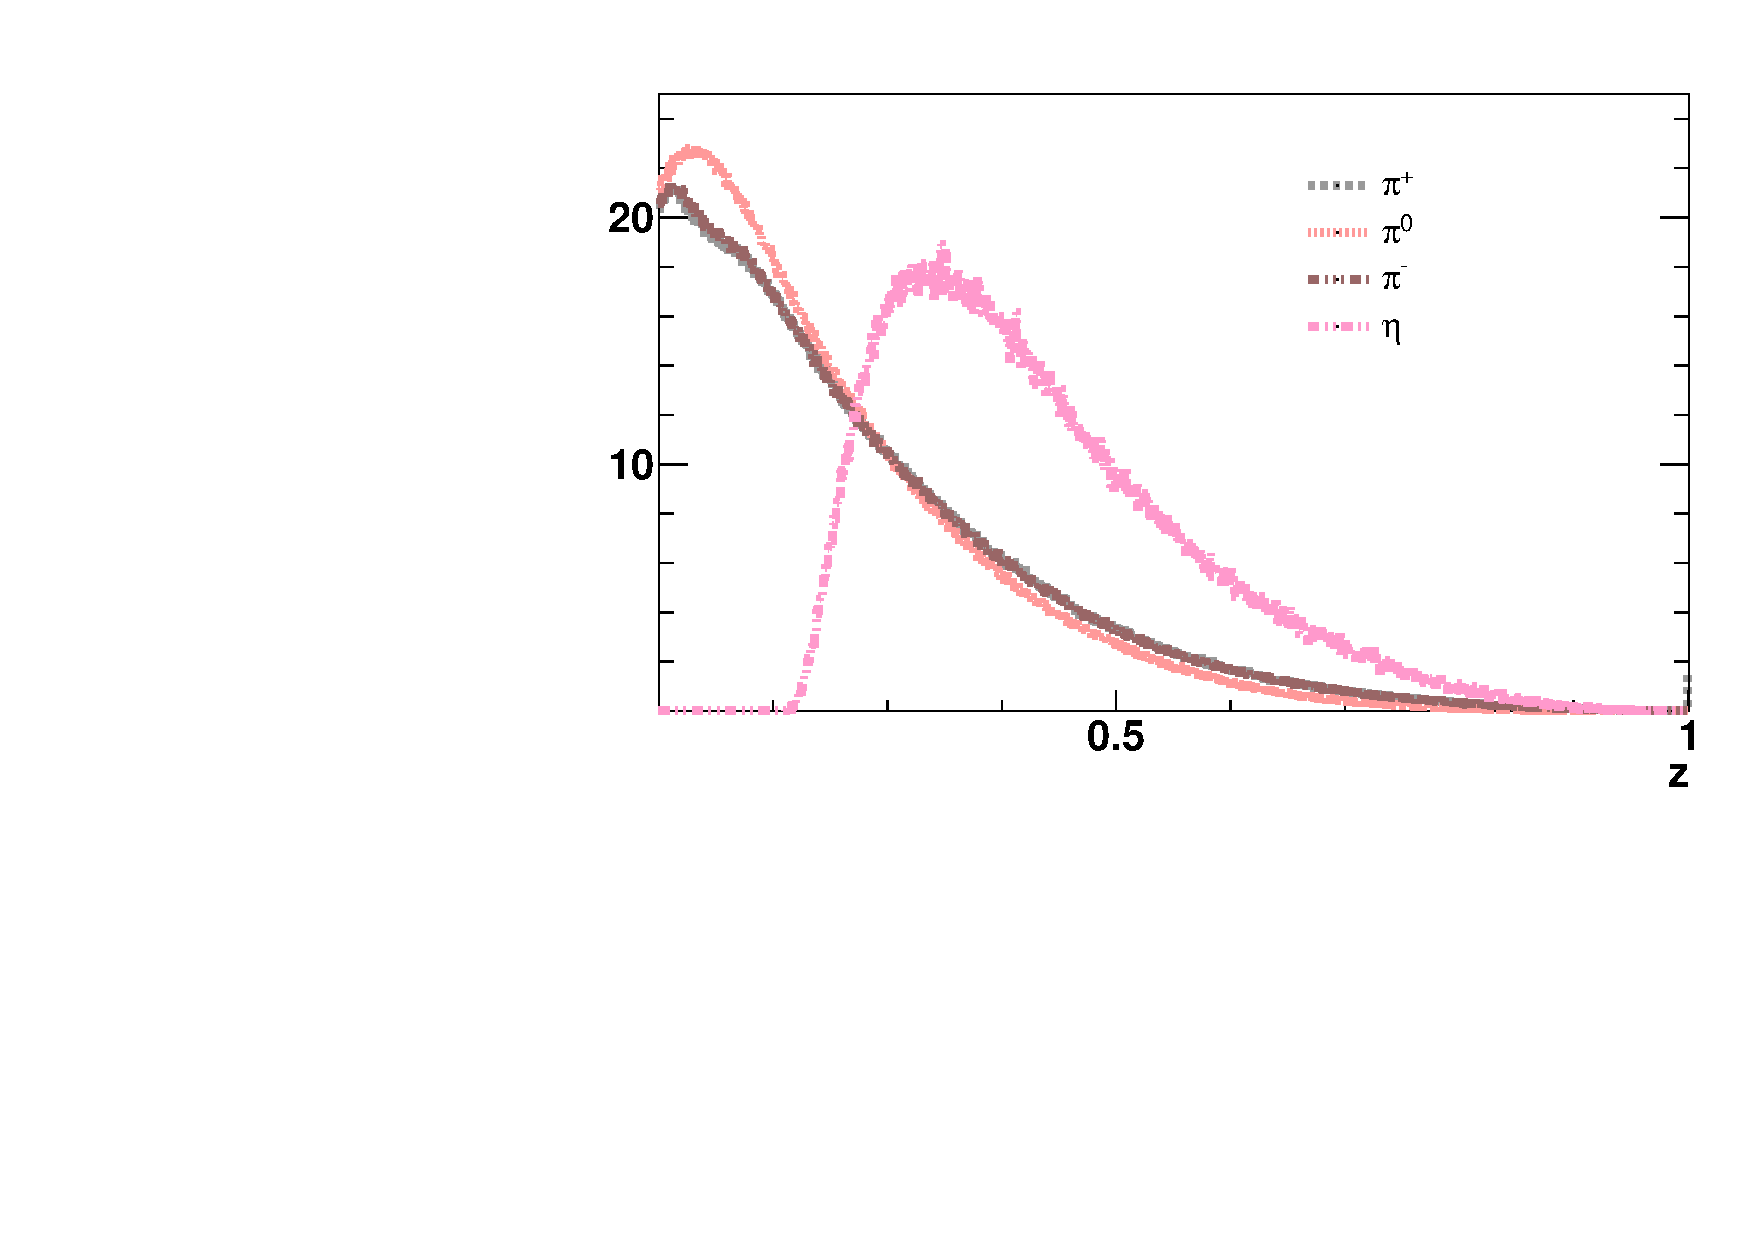
\includegraphics[width=.48\textwidth,natwidth=600,natheight=400]{figure_dataselection/Z_distri.pdf}}
  \subfigure[$P_t$ distribution of mesons]{\label{fig:pi0pt}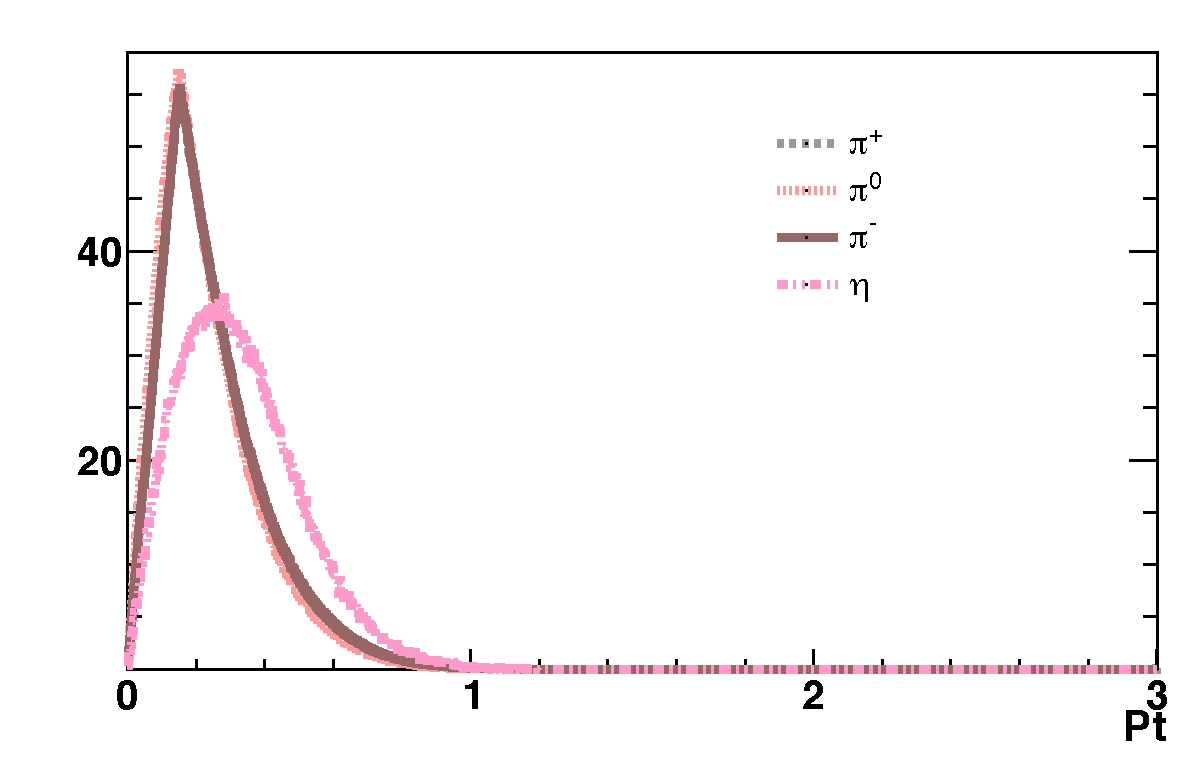
\includegraphics[width=.48\textwidth,natwidth=600,natheight=400]{figure_dataselection/Pt_distri.pdf}}
  \caption[Normalized kinematic distributions]{Normalized distribution of kinematic distributions with all event selection, fiducial requirements and the neutral meson reconstruction criteria (see section~\ref{sec:neutralmesonreconstruction}) applied with the exception of the $z$ cut. Left plot is the $z$ distribution of experimental data. The right plot is $P_t$ distribution. The $z$ distribution of the $\eta$ distribution is shifted with respect to the pions due to the higher mass and higher photon energy cut of the $\eta$. In ratios involving the $\eta$ we can remedy this by applying an appropriate $z$ cut on the pions as well. As shown in the appendix Sec.~\ref{sec:kinedistri_eta} the kinematic distributions of $\eta$ and pions is in good agreement for the same $z$ bin. }
  \label{fig:zptdistri}
\end{figure}

Two kinds of kinematic bins have been studied. In order to study both kinematic dependences the first hadron of the hadron pair is either binned in $z$ or $P_t$ according to the bin boundaries given in Tables~\ref{tab:whatissinglez} and~\ref{tab:whatissinglept}. For the neutral/charged mixed hadron pairs, we take the neutral hadron as the first hadron in a hadron pair and the kinematics of first hadron will be labeled with index $1$. While for charged hadron pairs we randomly pick one hadron as the first one. For the binnings that depend solely on $z$ or $P_t$, the bin number is determined by the first hadron and the dependence on $z_2$ and $P_{t2}$ is integrated out. 
\begin{table}[H]\small
\centering
\begin{tabular}{|l|l|l|l|l|l|l|l|l|}
\hline
$z_1$ bins & 0 &  1 & 2 & 3 & 4 & 5 & 6  \\ \hline
 $z_1$  & {\color{red}0.1$\textup{--}$0.2} & 0.2$\textup{--}$0.3 & 0.3$\textup{--}$0.4 & 0.4$\textup{--}$0.5 & 0.5$\textup{--}$0.6 & 0.6$\textup{--}$0.7 & 0.7$\textup{--}$1  \\ \hline
\end{tabular}
\caption[Bin boundaries for $z_1$  in the analysis of 1d dependences]{Bin boundaries for the first-hadron's fractional energy $z_1$ used in the analysis of one-dimensional dependences of the Collins effect. The first $z$ bin, indicated in red, will only be used in the $(z_1,z_2)$  binning. See text for more details.}
\label{tab:whatissinglez}
\end{table}
The Collins effect of the lowest $z$ bin is expected to be small since on average low $z$ particles are produced after multiple string breaks in the fragmentation process, losing spin information in the process. In addition, we show later in Section~\ref{sec:fiducialcut} that remaining detector effects are strongest for this $z$ bin. Therefore we drop this bin by introducing a cut of $z>0.2$ for all binnings where we integrate over $z$, as for those the lowest $z$ bin with its high statistics would mainly dilute the measurement. Nevertheless, we keep the bin for the $(z_1,z_2)$ binning.


\begin{table}[H]\small
\centering
\begin{tabular}{|l|l|l|l|l|l|l|l|l|l|l|l|l|l|l|l|l|l|}
\hline
 $P_{t1}$ bins & 0 &  1 & 2 & 3   \\ \hline
 $P_{t1}$ (GeV)  & 0$\textup{--}$0.15& 0.15$\textup{--}$0.3 & 0.3$\textup{--}$0.5 & 0.5$\textup{--}$3  \\ \hline
\end{tabular}
\caption[Bin boundaries for  $P_{t1}$  in the analysis of 1d dependences]{Bin boundaries for the first-hadron's transverse momentum $P_{t1}$ used in the analysis of one-dimensional dependences of the Collins effect.}
\label{tab:whatissinglept}
\end{table}

In addition to studying the dependence of the asymmetry on the kinematics of the first hadron (integrating over the dependence on the second hadron),  we also study the dependence of the asymmetry on both hadrons. 
In previous charged-pion analyses, a reduced binning  as shown in Fig.~\ref{fig:comz_mark} was used where additional bin combinations were eliminated that are symmetric under the interchange of the particle order.
\begin{figure}[H]
\centering
\begin{minipage}{.5\textwidth}
  \centering
  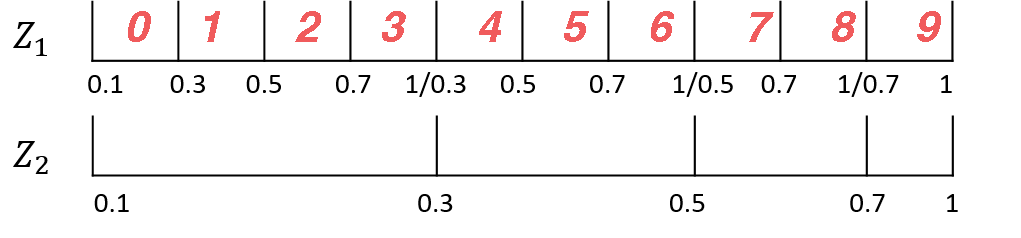
\includegraphics[width=0.95\textwidth,natwidth=610,natheight=642]{figure_dataselection/zbin.pdf}
  \captionof{figure}{$(z_1,z_2)$ bins used in pervious charged-pion analysis.}
  \label{fig:comz_mark}
\end{minipage}%
\end{figure}

In contrast, in the present analysis we consider combinations where the hadrons have different flavor content or iso-spin and therefore
the non-reduced  binning shown in Fig.~\ref{fig:binnings} is employed. To further investigate the dependence of the asymmetry on $z$ and $P_t$ simultaneously, we also used a binning differential in $z$ and $P_t$ of the first hadron as indicated in Fig.~\ref{fig:zptbin}.   

\begin{figure}[H]
\captionsetup[subfloat]{farskip=2pt,captionskip=1pt}
\centering
\subfigure[$(z_1,z_2)$ bins]{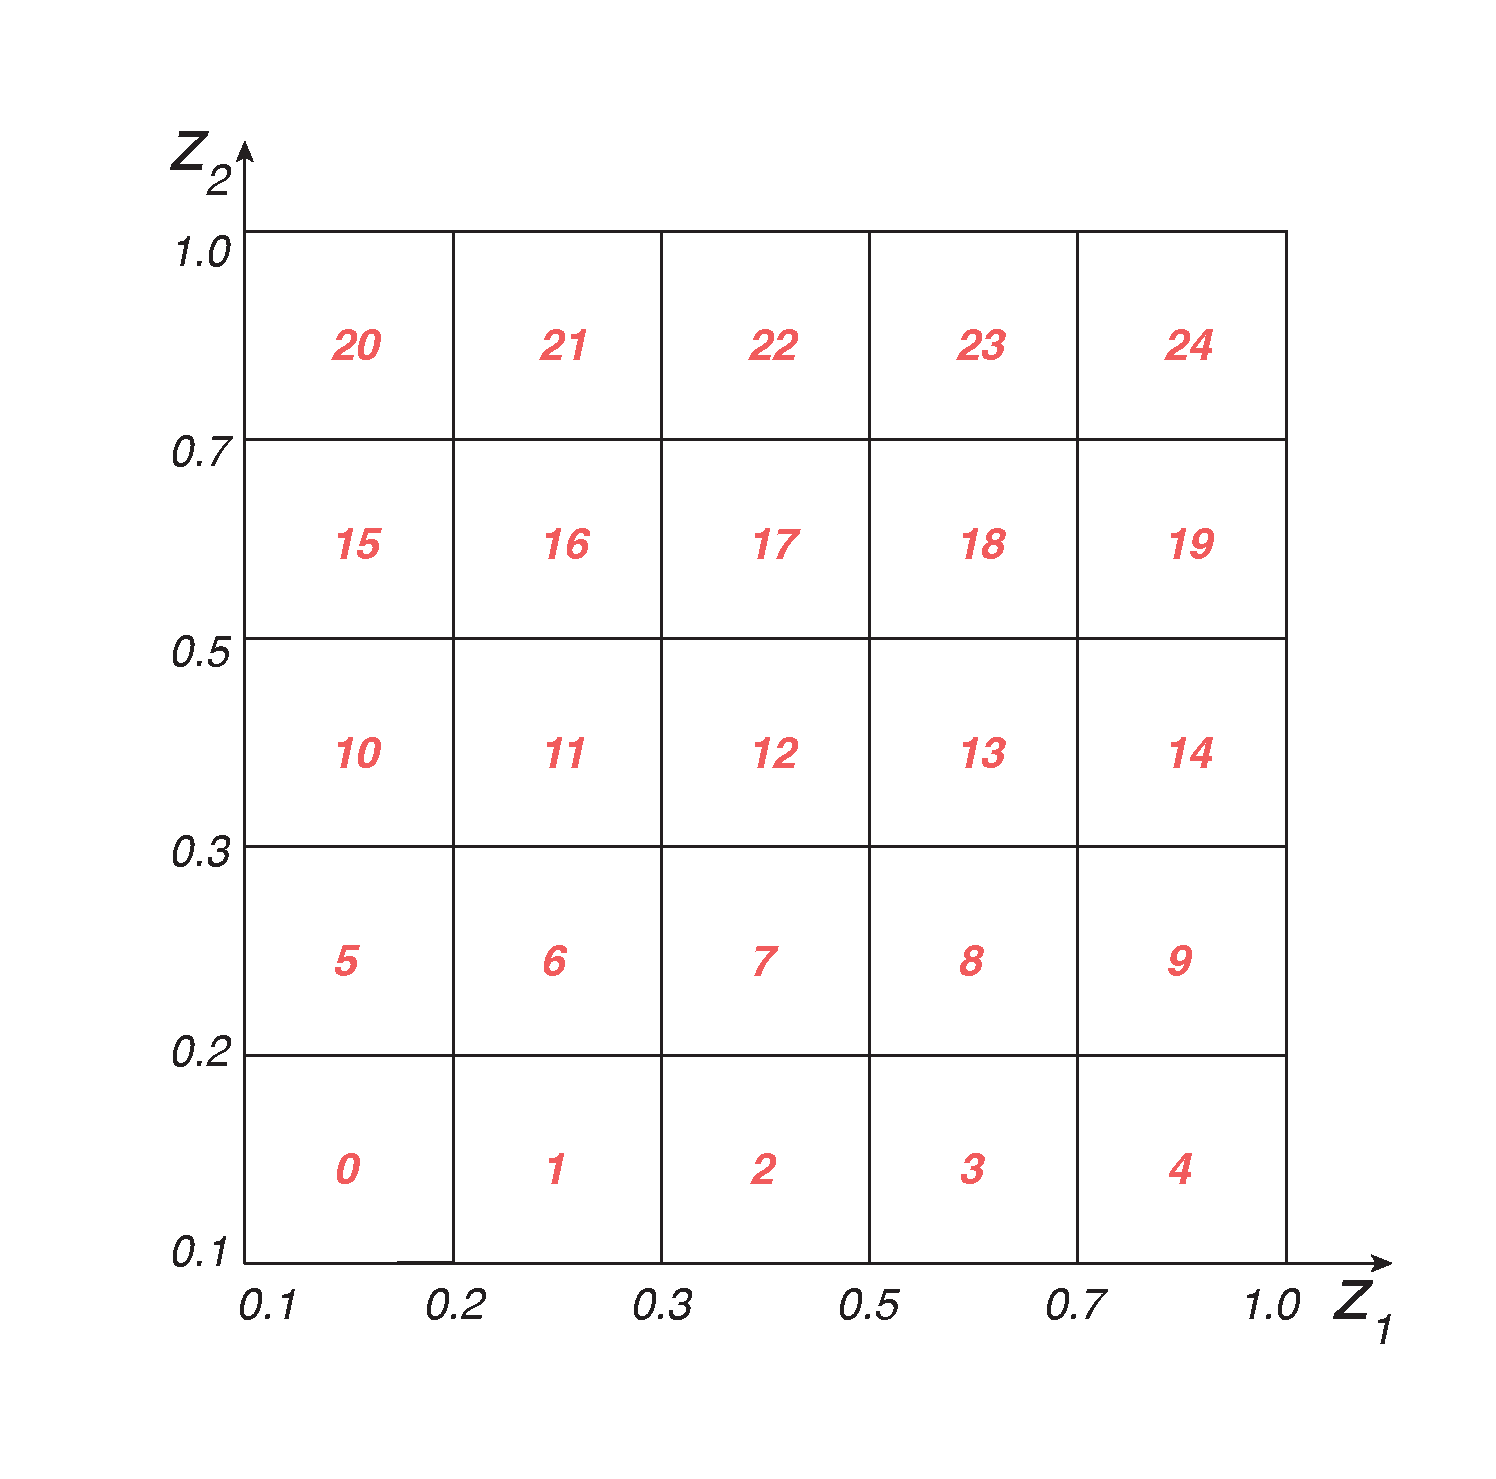
\includegraphics[width=.48\textwidth,natwidth=250,natheight=100]{figure_dataselection/comzbin.pdf}\label{fig:z1z2binning}}
\subfigure[$(P_{t1},P_{t2})$ bins]{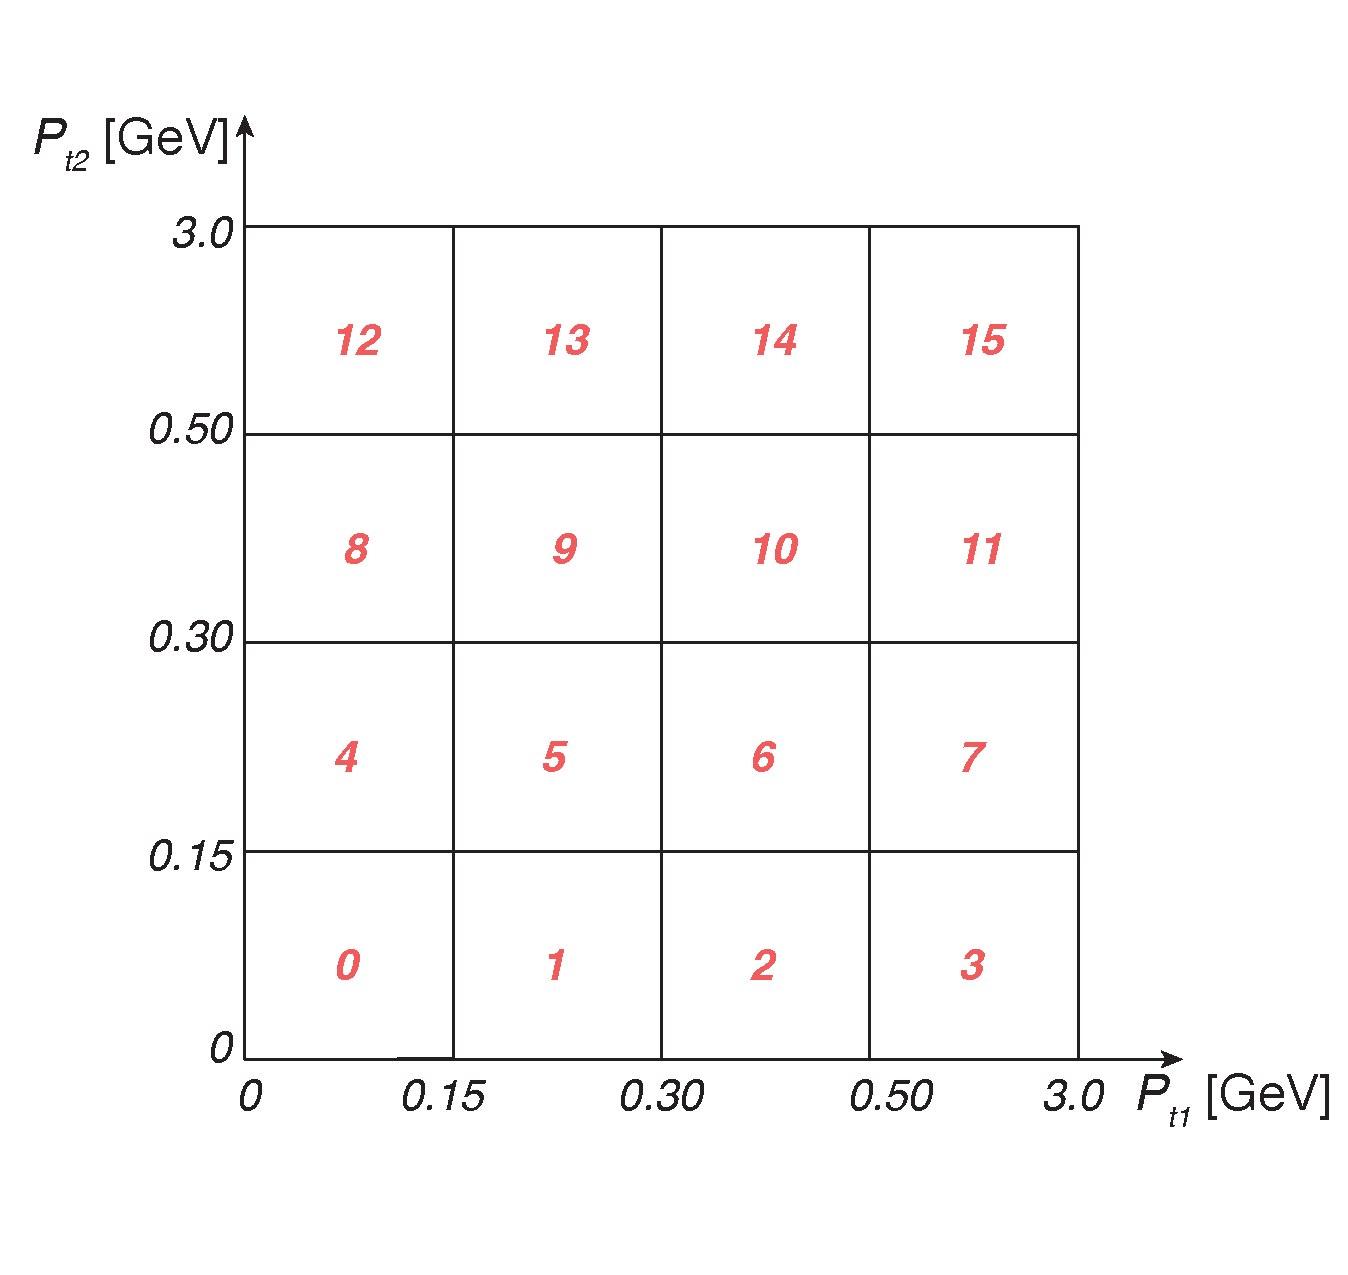
\includegraphics[width=.48\textwidth,natwidth=250,natheight=100]{figure_dataselection/comptbin.pdf}\label{fig:pt1pt2binning}}
\caption[Bin boundaries and numbering for the 2d binning in $z$ or $P_{t}$ of the two hadrons]{Bin boundaries and numbering for the (hadron1, hadron2) bins. The index of the bin is indicated as a red number.}
\label{fig:binnings}
\end{figure}

\begin{figure}[H]
    \centering
    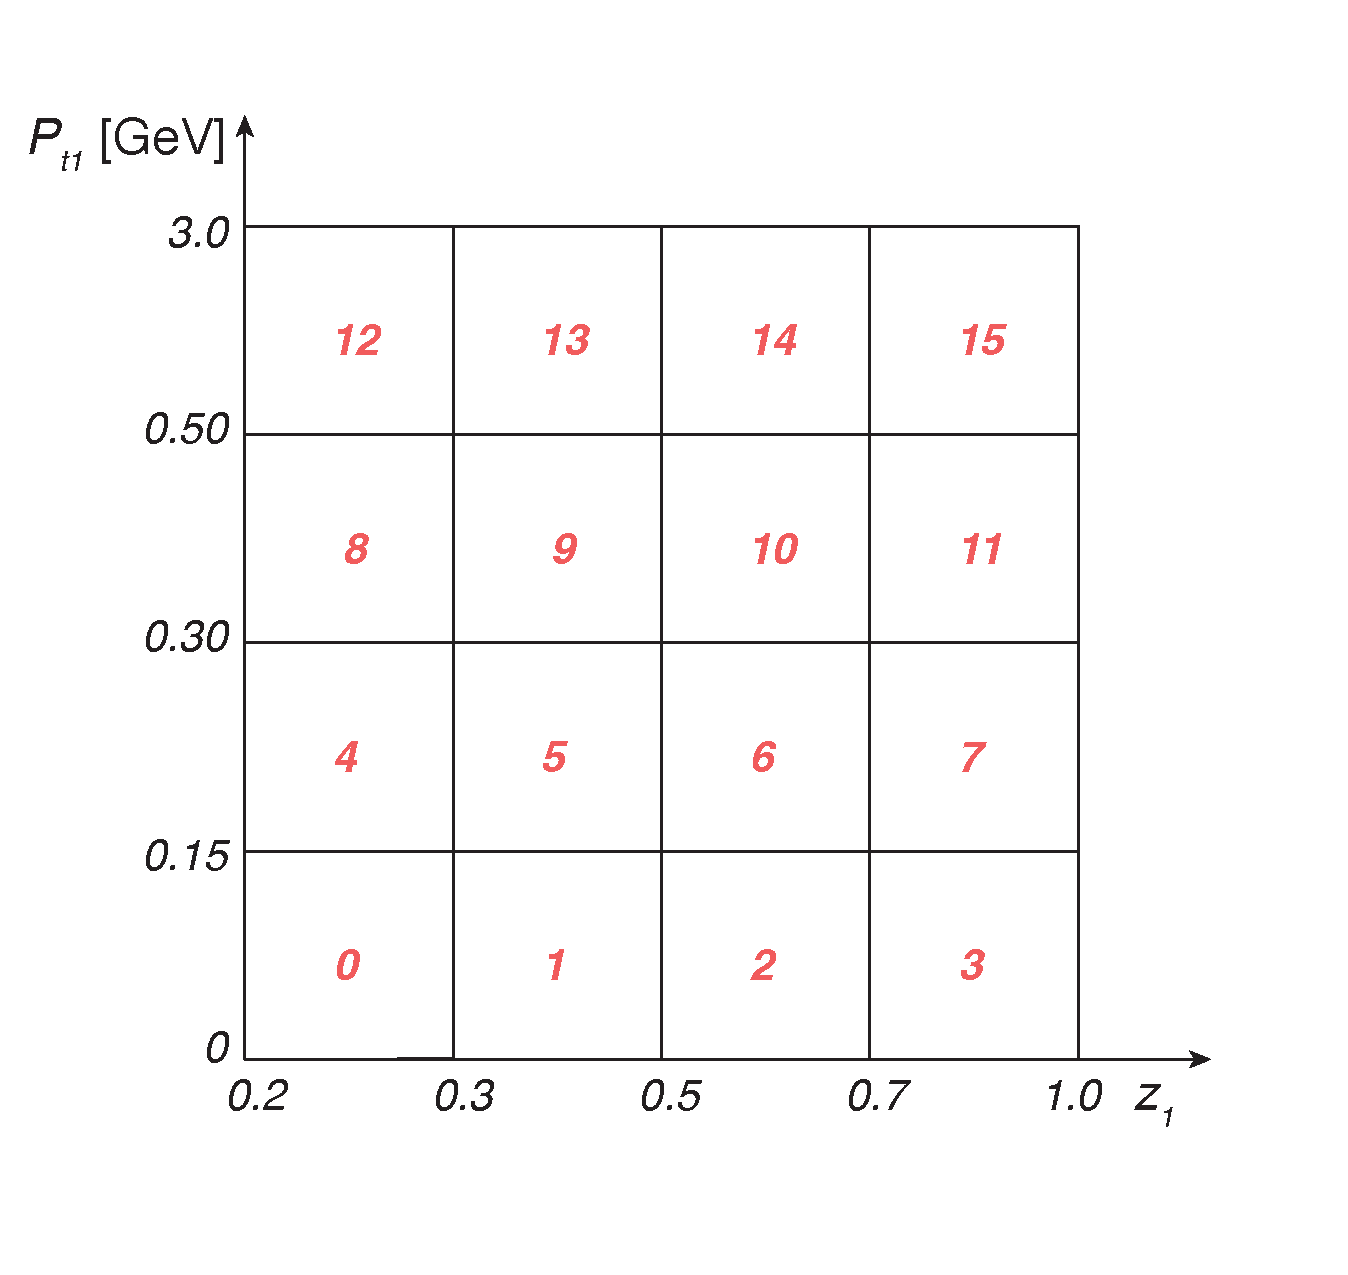
\includegraphics[width=0.5\textwidth,natwidth=250,natheight=100]{figure_dataselection/zptbin.pdf}
    \caption{Bin boundaries and numbering for the mixed 2d binning of the first-hadron's $z$ and $P_t$.}
    \label{fig:zptbin}
\end{figure}



%%%%%%%%%%%%%%%%%%%%%%%%%%%%%%%%%%%%%%%%%%%


\subsection{Fiducial and Energy Constraints for Hadron Selection}
\label{sec:fidAndEnergyCuts}
In the following we discuss the fiducial cuts and photon energy constraints on the hadron selection. The fiducial cuts are defined in terms of an opening angle of the hadron or photon with respect to the
thrust axis. This is discussed in detail in Section~\ref{sec:fiducialcut} below. We use a grid search on the fiducial cuts and the photon energy to find constraints that optimize the figure-of-merit (FOM) $\nicefrac{S}{\sqrt{N}}$ . This initial set of fiducial cuts is then refined to equalize kinematic distributions between the different hadron species.

\subsubsection{\texorpdfstring{Energy Constraint for $\gamma$ and mesons}{Energy Constraint for gamma and mesons}}
\label{sec:energyconstraint}


The $\gamma$ energy threshold and energy asymmetry are studied to reduce the background. A higher threshold leads to purer data at the expense of yield loss. Similarly, a tighter energy-asymmetry requirement should also improve the signal purity while reducing the yield. However, it was found that an asymmetry cut in addition to the energy-threshold cut does not improve the FOM significantly and we did not apply an asymmetry cut.
%as shown in Fig~\ref{fig:photon_asymmetry}
%\begin{figure}[H]
%\centering
  %\subfigure[]{\label{fig:photon_asymmetry1}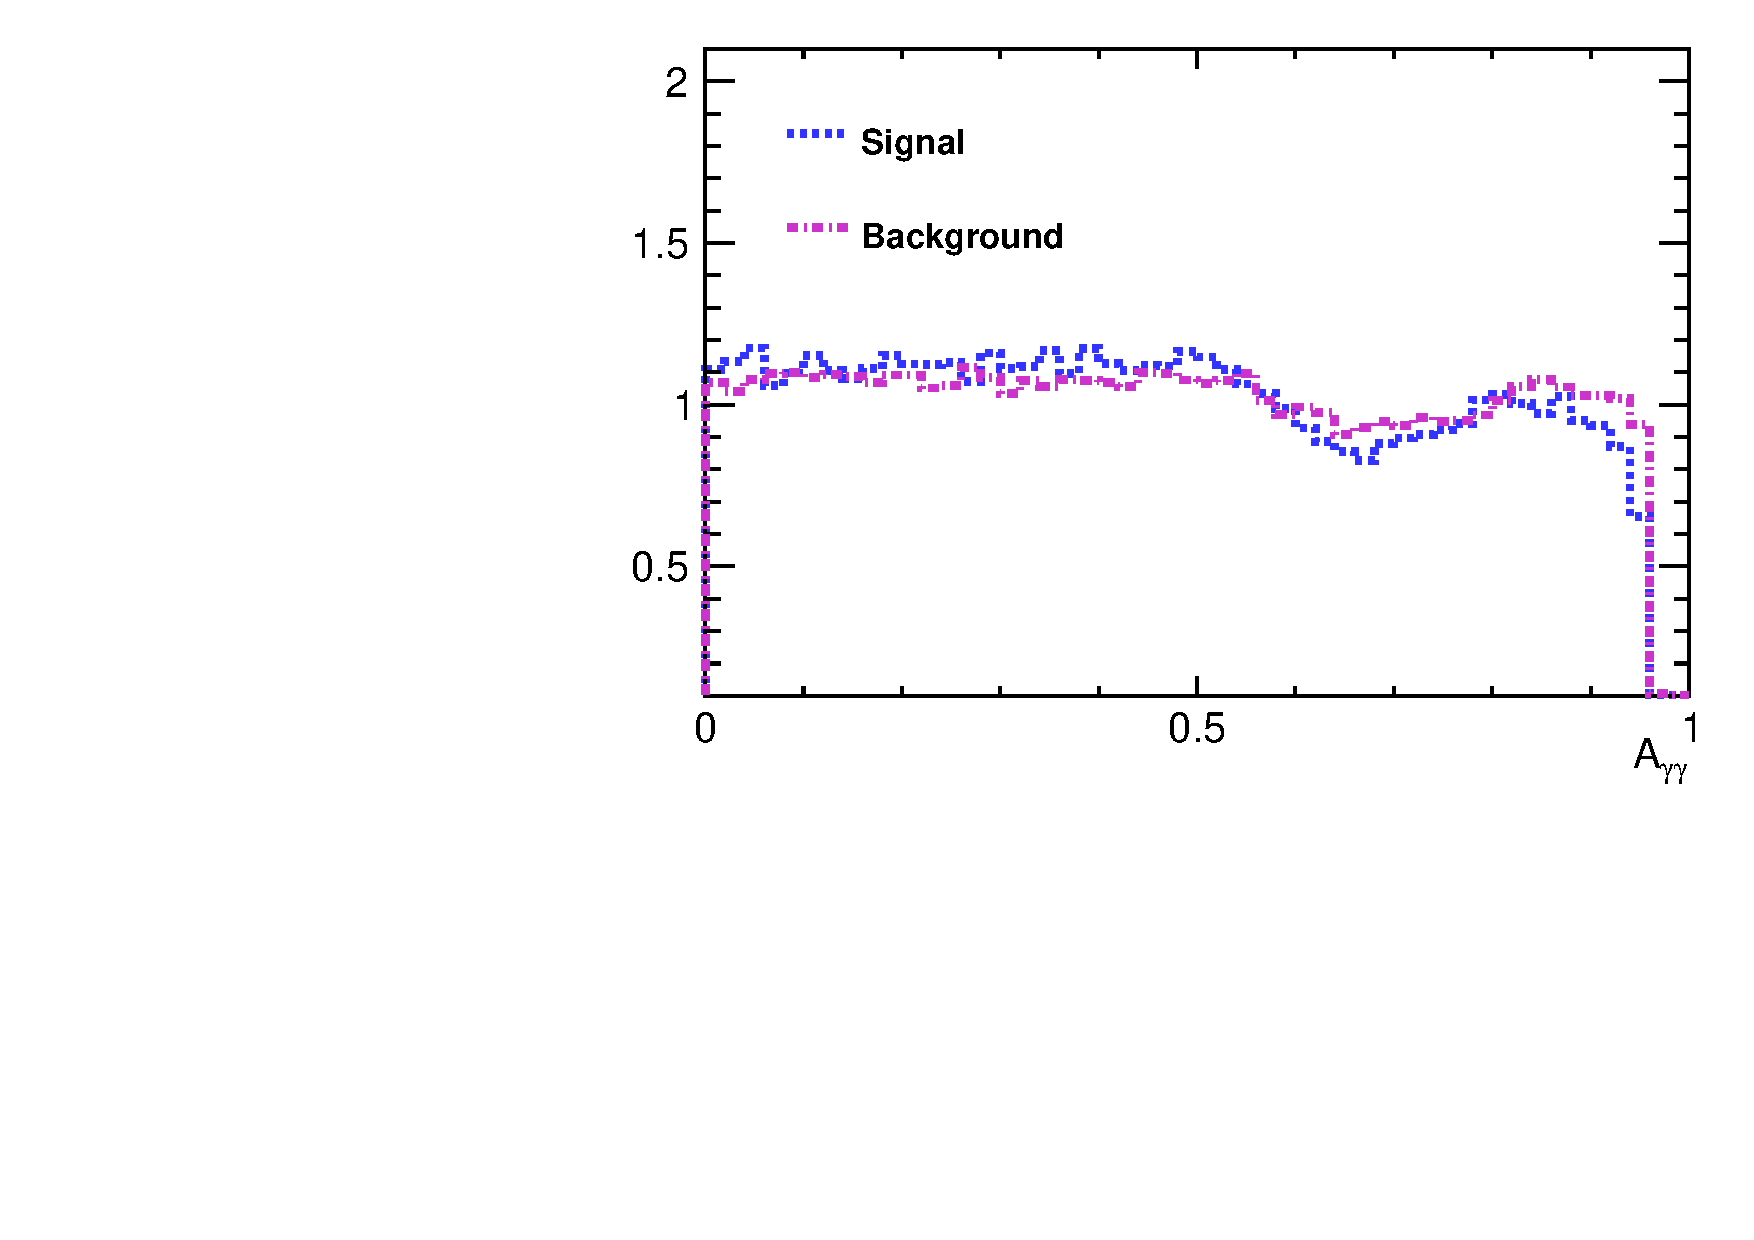
\includegraphics[width=.48\textwidth,natwidth=250,natheight=100]{figure_dataselection/pi0_asy_plot_Z3.pdf}}
  %\subfigure[]{\label{fig:photon_asymmetry2}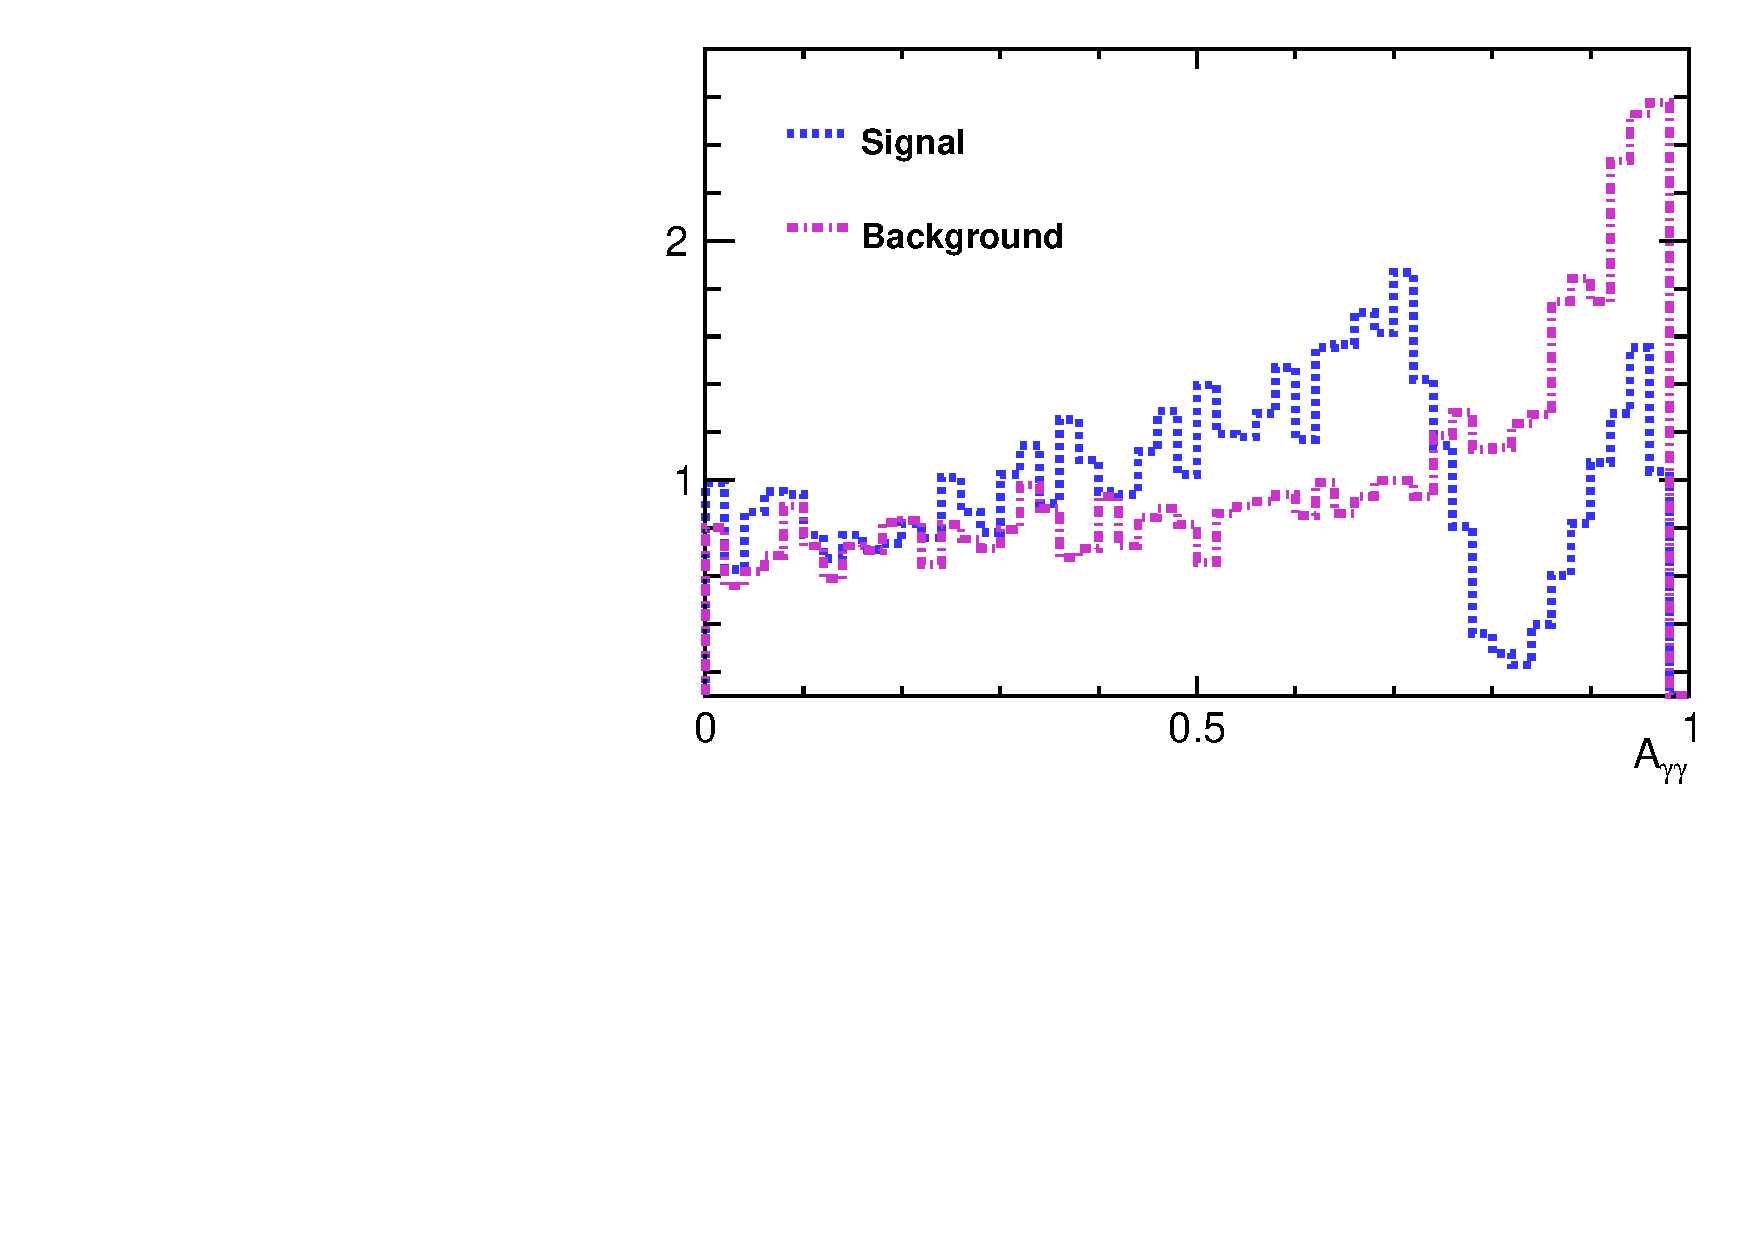
\includegraphics[width=.48\textwidth,natwidth=250,natheight=100]{figure_dataselection/pi0_asy_plot_Z6.pdf}}
 % \caption{Two examples of energy asymmetry $A_{\gamma\gamma}$. The left plot shows the $0.4<z<0.5$ bin and right plot the $0.7<z<1.0$ bin. In each plot, the blue line is the signal energy asymmetry andthe  purple line is the background energy asymmetry. To make the plots, the invariant mass of the reconstructed $\pi^0$ is restricted in the range of $0.1$~GeV$\textup{--}0.18$~GeV to avoid contribution of $\eta$ or other irrelevant background. As MC data is used in this plot, the signal and background events are distinguished by the particle ID of the reconstructed particles as well as the ID of their parents.}
%\label{fig:photon_asymmetry}
%\end{figure}

For the grid search discussed later, we consider the following bins in photon energy and photon-energy asymmetry:
\begin{itemize}
  \item Photon Energy:
    \begin{itemize}
      \item $\pi^{0}$: $50$~MeV, $100$~MeV, $150$~MeV 
      \item $\eta$: $150$~MeV, $200$~MeV, $250$~MeV, $300$~MeV, $400$~MeV
    \end{itemize}
  \item Photon Energy asymmetry $A_{\gamma\gamma}=\frac{|\gamma_1-\gamma_2|}{\gamma_1+\gamma_2}$ : $<0.8$ ,$<0.9$, $<1$
\end{itemize}



\subsubsection{Fiducial Constraints}
\label{sec:fiducialcut}
Since we extract modulations that are only expected to be a few percent of the total cross-section, we restrict our analysis to parts of the detectors where the acceptance is smooth. This means that we apply fiducial cuts that ensure that all $\gamma$'s are captured in the barrel EMCAL shown in Fig.~\ref{fig:2}. In the CMS, where we define our fiducial constraints, this corresponds to a cut on the polar angle of  hadrons and $\gamma$'s of 0.84~rad $<\theta<2.53$~rad, where $\theta$ is the angle between momentum direction and the $e^+e^-$ axis.
  In addition, because we are measuring azimuthal asymmetries around the thrust axis, we apply fiducial cuts on the opening angle (OA) of the detected hadrons/photons with respect to the thrust axis ($H_{OA}$ and $\gamma_{OA}$, respectively), such that the acceptance of the detector does not lead to large false asymmetries. This is the case when the acceptance is azimuthally symmetric around the thrust axis for all allowed directions of that axis and is illustrated in Fig.~\ref{fig:FiducialCut}. 

\begin{figure}[H]
  \centering
  \includegraphics[width=0.8\textwidth,natwidth=610,natheight=642]{figure_dataselection/EMCAL.pdf}
  %\includegraphics[scale=.3,keepaspectratio]{EMCAL.pdf}
  \caption{Configuration of Belle electromagnetic calorimeter~\cite{BelleDetector}.}
  \label{fig:2}
\end{figure}

\begin{figure}[H]
  \centering
  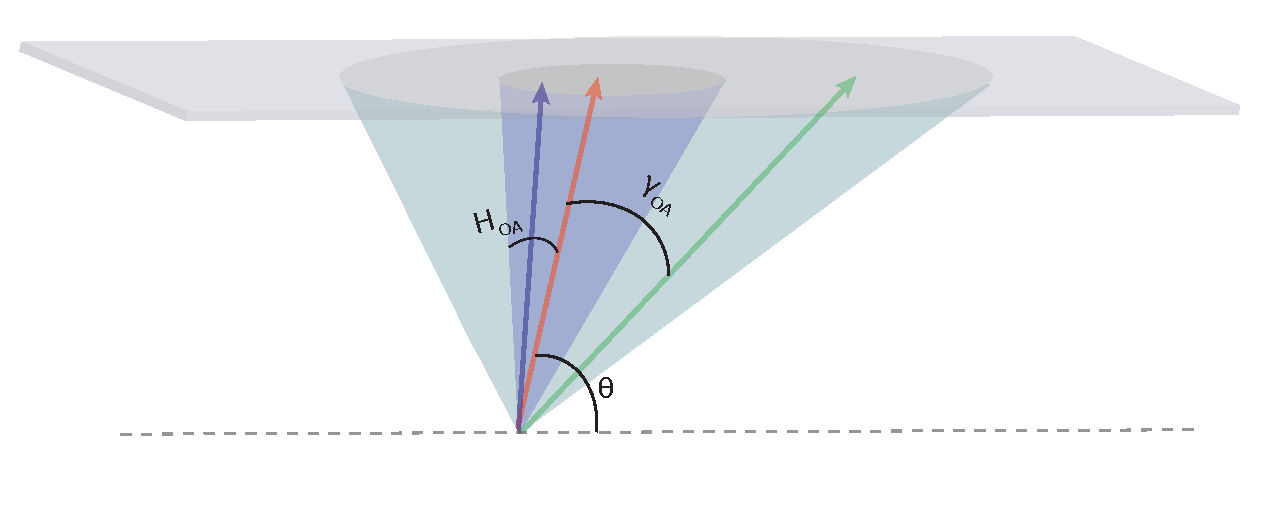
\includegraphics[width=0.95\textwidth,natwidth=610,natheight=642]{figure_dataselection/OA.pdf}
  \captionof{figure}[Illustration of the fiducial constraints in the CMS system.]{Illustration of the fiducial constraints in the CMS system. The red line represents the thrust axis, the green line a photon and the blue line a hadron. The cones represent the corresponding boundaries ($H_{OA}$ should be drawn between the hadron, not the blue boundary, and the thrust axis). The outer cone stand for the boundary of $\gamma$'s and the inner cone for hadrons. To make sure that all $\gamma$s are captured by the barrel EMCAL, the value of $\theta \pm \gamma_{OA}$ should fall in the range $0.84~\text{rad}<\theta\pm \gamma_{OA}<2.53~\text{rad}$. Here $\theta$ is again the angle between the $e^+e^-$ beam axis and the thrust axis in the CMS.}
  \label{fig:FiducialCut}
\end{figure}
 
 Given the fiducial cuts described above, the OA constraint also dictates the allowed range of the polar angle $\theta$ of the thrust axis to the beam axis in the CMS.  Even at maximal OA, tracks and photons have to be contained in the allowed polar-angle range given by the EMCAL acceptance. For example, if the maximum OA is $0.4$~rad, the thrust direction is limited within $1.24~\text{rad}<\theta<2.13~\text{rad}$.  A tighter boundary of OA leaves more room for thrust range at the expense of the yield of hadrons, and vice versa as shown in Fig.~\ref{fig:OAs}. For the grid search we use (in addition to the previously defined bins in photon energy and asymmetry) the following bins in the opening angle:
\begin{itemize}
\item Opening angle (OA): $<0.4$~rad, $<0.5$~rad, $<0.6$~rad.
\end{itemize}

As already indicated in~Fig.~\ref{fig:FiducialCut}, we will eventually apply a tighter OA cut on hadrons than on the photons, since our goal is to have similar kinematics for charged and neutral hadrons and the decay photons of the neutral hadrons can occupy a larger OA than the parent hadron. In a first step we determine the optimal fiducial cuts using simulated data under the assumption that we will use the same cuts for $H_{OA}$ and $\gamma_{OA}$.  In a second step we choose a subset of the thus allowed phase space for $H_{OA}$ by applying tighter bounds to equalize the kinematic distributions between the different hadron species.

Table~\ref{tab:FOM} shows the optimized constraints for each kinematic bin. Most bins of $\pi^0$ have the same optimized constraints, namely the photon-energy threshold of $50$~MeV, no photon-energy asymmetry cut and an OA constraint of $0.5$, and these constraints are chosen as our data selection criteria. For other bins, comparisons are made to confirm that the FOMs of selected criteria of that bin approximate the optimized FOM. The same approach is used for $\eta$ and the final selection criteria can be found in Table~\ref{tab:constrain}.%includes the photon energy threshold $250$~MeV, no photon energy asymmetry cut and OA constraint $0.5$. With $z<0.3$ the purity of $\eta$ is below $30\%$ and thus it is required that $z>0.3$ for $\eta$ mesons. 
\begin{table}[t]
\begin{tabular}{|p{1.3cm}|l|l|l|l|l|l|l|l|l|l|l|l|l|}
\hline
Bin & $E_{\gamma}$ [MeV] & $A_{\gamma\gamma}$ & OA \\ \hline
$z_0$ & 0.05 & 0.8 & 0.6 \\\hline
$z_1$ & 0.05 & 0.9 & 0.5 \\\hline
$z_2$ & 0.05 & 1 & 0.5 \\\hline
$z_3$ & 0.05 & 1 & 0.5 \\\hline
$z_4$ & 0.10 & 1 & 0.5 \\\hline
$z_5$ & 0.05 & 1 & 0.5 \\\hline
$z_6$ & 0.05 & 1 & 0.5 \\\hline
$P_{t0}$ & 0.05 & 1 & 0.5 \\\hline
$P_{t1}$ & 0.05 & 1 & 0.5 \\\hline
$P_{t2}$ & 0.10 & 1 & 0.5 \\\hline
$P_{t3}$ & 0.05 & 1 & 0.6 \\\hline
\end{tabular}
%\caption{Constraints that generate optimized FOM for $\pi^{0}$.}
%\label{tab:pi0FOM}
\quad
\begin{tabular}{|p{1.3cm}|l|l|l|l|l|l|l|l|l|l|l|l|l|}
\hline
Bin & $E_{\gamma}$ [MeV] & $A_{\gamma\gamma}$ & OA \\ \hline
$z_0$ &  &  &  \\\hline
$z_1$ &  &  &  \\\hline
$z_2$ & 0.15 & 1 & 0.5 \\\hline
$z_3$ & 0.25 & 1 & 0.5 \\\hline
$z_4$ & 0.25 & 1 & 0.5 \\\hline
$z_5$ & 0.25 & 1 & 0.5 \\\hline
$z_6$ & 0.25 & 1 & 0.5 \\\hline
$P_{t0}$ & 0.20 & 1 & 0.5 \\\hline
$P_{t1}$ & 0.20 & 1 & 0.5 \\\hline
$P_{t2}$ & 0.15 & 1 & 0.5 \\\hline
$P_{t3}$ & 0.25 & 1 & 0.5 \\\hline
\end{tabular}
\caption[Constraints that generate optimized FOM for $\pi^0$ and $\eta$]{Constraints that generate optimized FOM for $\pi^0$~(left) and $\eta$~(right).}
\label{tab:FOM}
\end{table}


\begin{figure}[h]
  \centering     %%% not \center
  \subfigure[$\pi^0$ to thrust angle]{\label{fig:a}\includegraphics[width=60mm]{figure_dataselection/pi0_OA.eps}}
  \subfigure[$\eta$ to thrust angle]{\label{fig:b}\includegraphics[width=60mm]{figure_dataselection/eta_OA.eps}}
  \caption[$H_{OA}$ distribution under various $\gamma_{OA}$ constraints]{$H_{OA}$ distribution under various $\gamma_{OA}$ constraints; the different color lines represent different $\gamma_{OA}$ constraints. The constraints are meant to be symmetric between the hemispheres, i.e. if  $\gamma_{OA}> \pi/2$ the constraint is on $\pi-\gamma_{OA} $.  For example, the $\gamma_{OA}$ constraint for the red solid line is 0.3~rad. It can be seen that with the decrease of the $\gamma$ range, the width of the hadron distribution becomes thinner.}
  \label{fig:OAs}
\end{figure}



%Fig.~\ref{fig:FiducialCut} shows the hadron/photon to thrust opening angles that will be used to do fiducial constraint. Our previous study shows that the optimized criteria for OA is $0.5$ for hadrons/photons. 
In addition, to avoid false asymmetries, the opening angle cut has to be chosen to match the $P_t$ and $z$ distributions between the neutral and charged hadrons used in the double ratio. Otherwise, the double ratio would be difficult to interpret, since the integration ranges for the different contributing hadrons in $P_t$ and $z$ would be different. Moreover, the cancelation of detector effects in the double ratio would not be guaranteed.
%However, the main motivation behind the opening cut is the goal to equalize the observed kinematic distributions between neutral and charged mesons. Given that the underlying distributions of $p_T$ and $z$ should be very similar, matching observed distributions for these variables imply matching detection efficiencies. This in turn is a prerequisite to successfully apply the double ratio method which is used to cancel detector effects.
In \cref{fig:kine_distri1,fig:kine_distri2,fig:kine_distri3,fig:kine_distri4} we compare different $H_{OA}$ constraints, where we leave $\gamma_{OA}$ at the previously determined optimum of $\gamma_{OA}<0.5$.
As expected, we see better agreement of the kinematic distribution of pions under tighter $H_{OA}$ constraints. More plots can be found in Appendix~\ref{sec:kinedistri_pi0} and~\ref{sec:kinedistri_eta}.
 
\begin{figure}[H]
\captionsetup[subfloat]{farskip=2pt,captionskip=1pt}
\centering
\subfigure[$H_{OA}<0.3$]{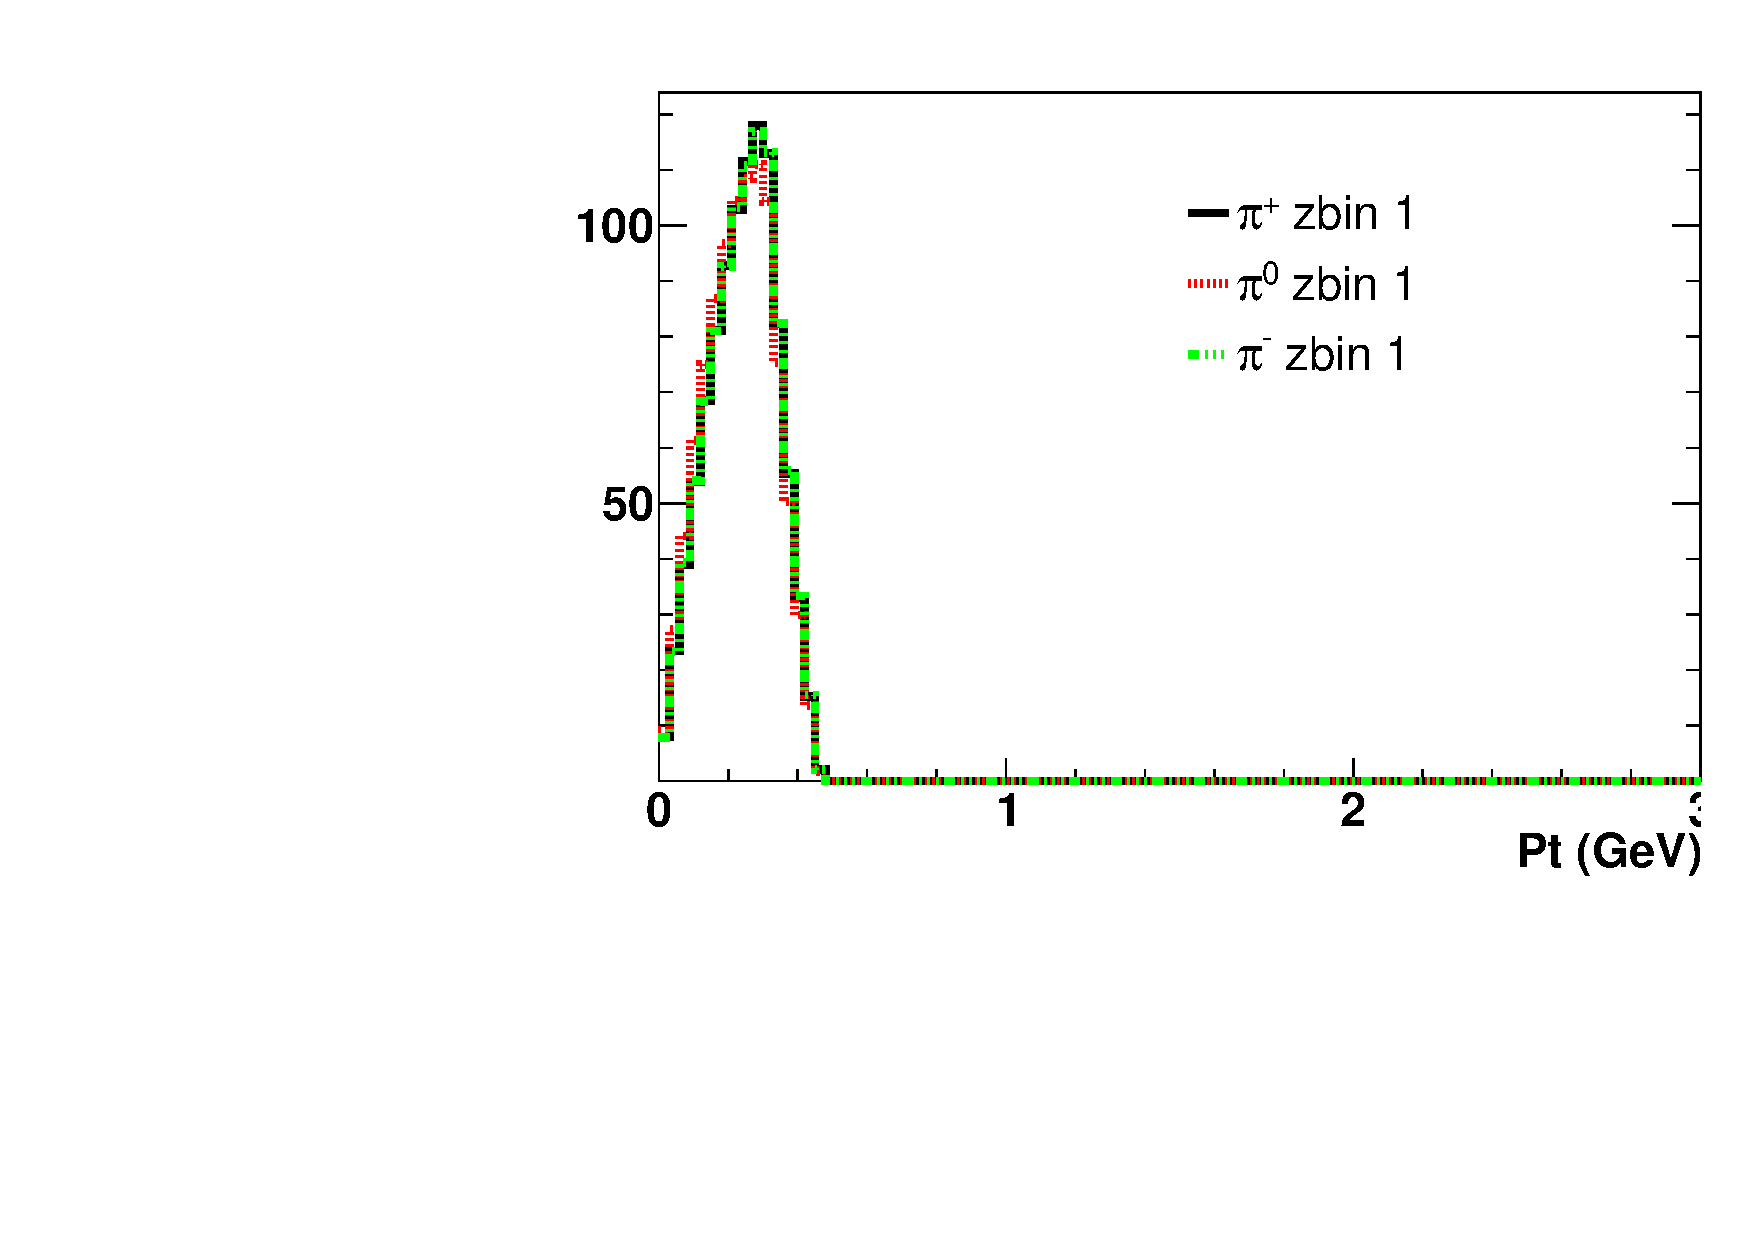
\includegraphics[width=.31\textwidth,natwidth=250,natheight=100]{figure_fiducial/had0.3/Pt_distri_for_zbin_1_norm_had03.pdf}\label{fig:kine_distri11}}
\subfigure[$H_{OA}<0.4$]{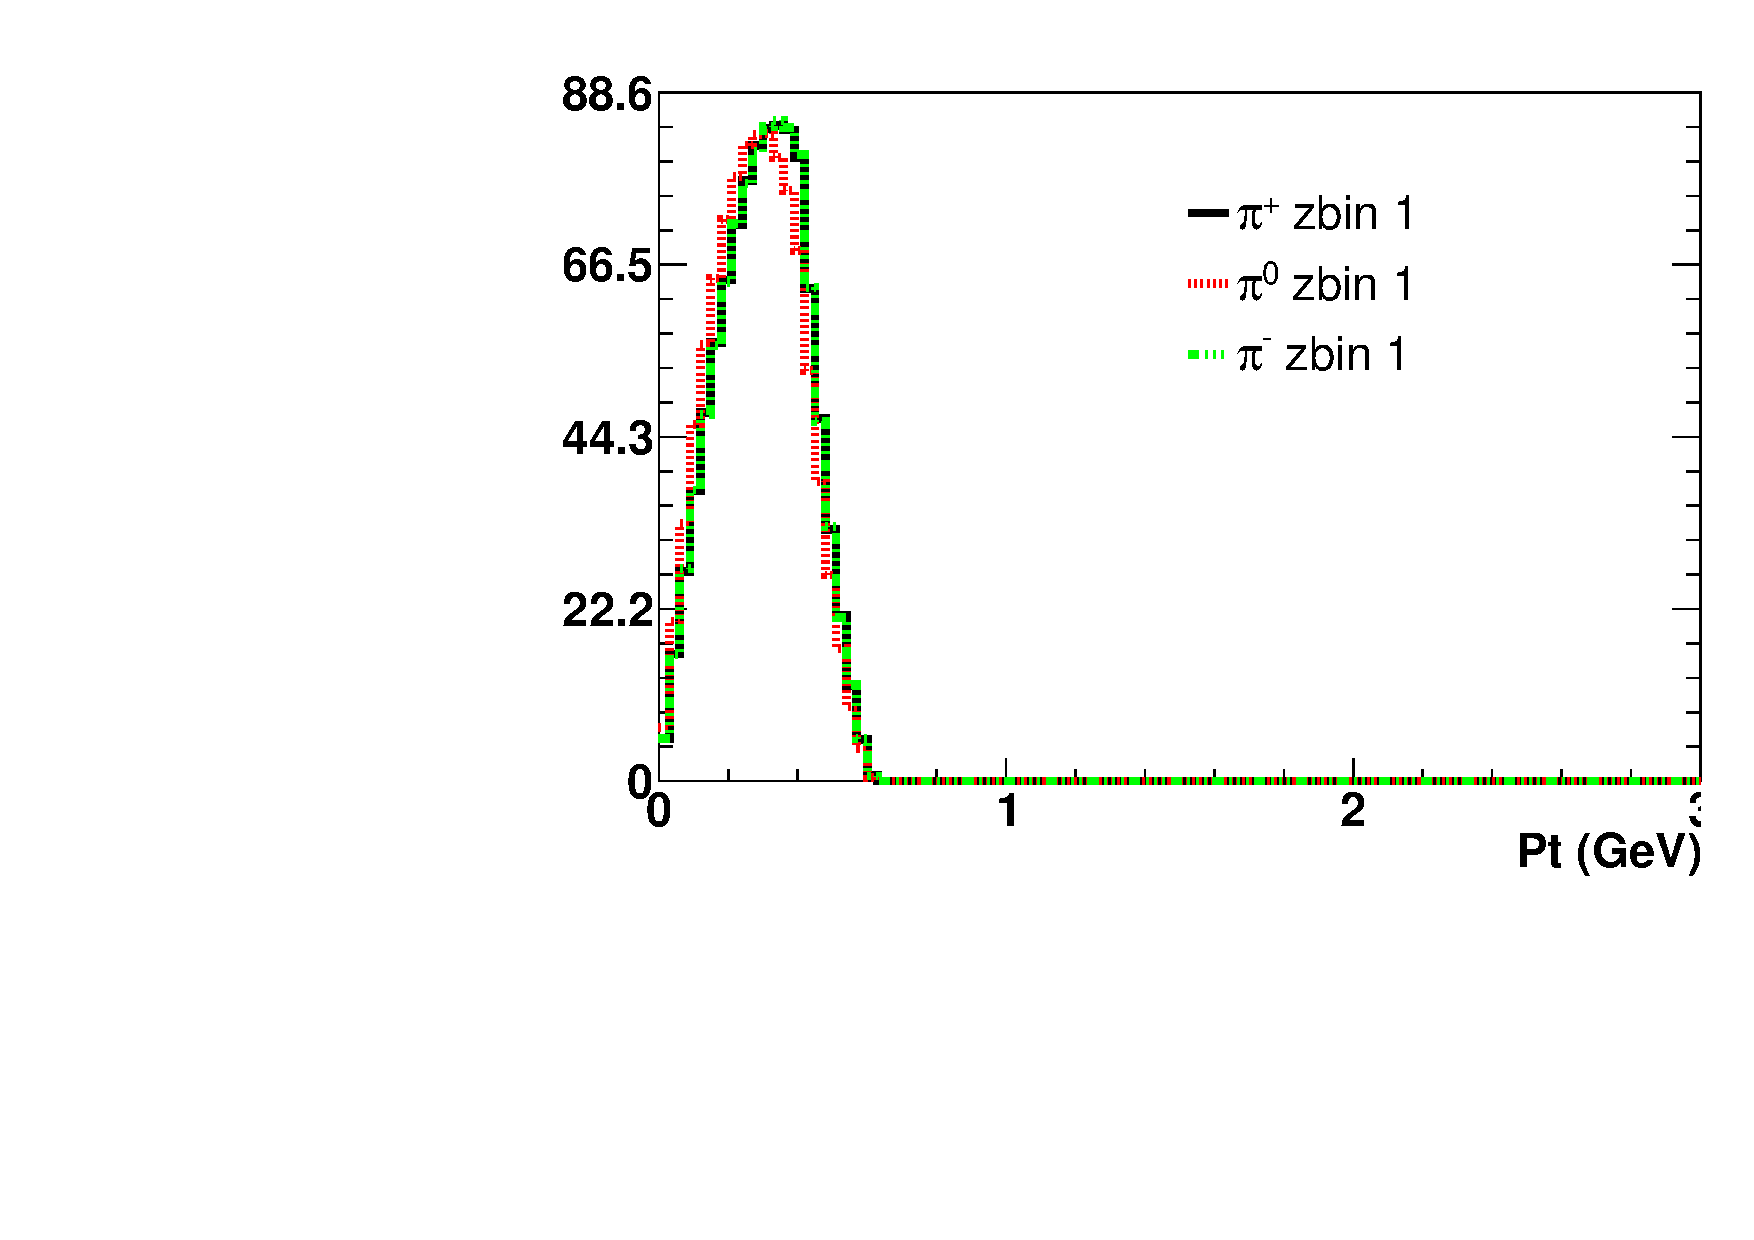
\includegraphics[width=.31\textwidth,natwidth=250,natheight=100]{figure_fiducial/had0.4/Pt_distri_for_zbin_1_norm_had04.pdf}\label{fig:kine_distri12}}
\subfigure[$H_{OA}<0.5$]{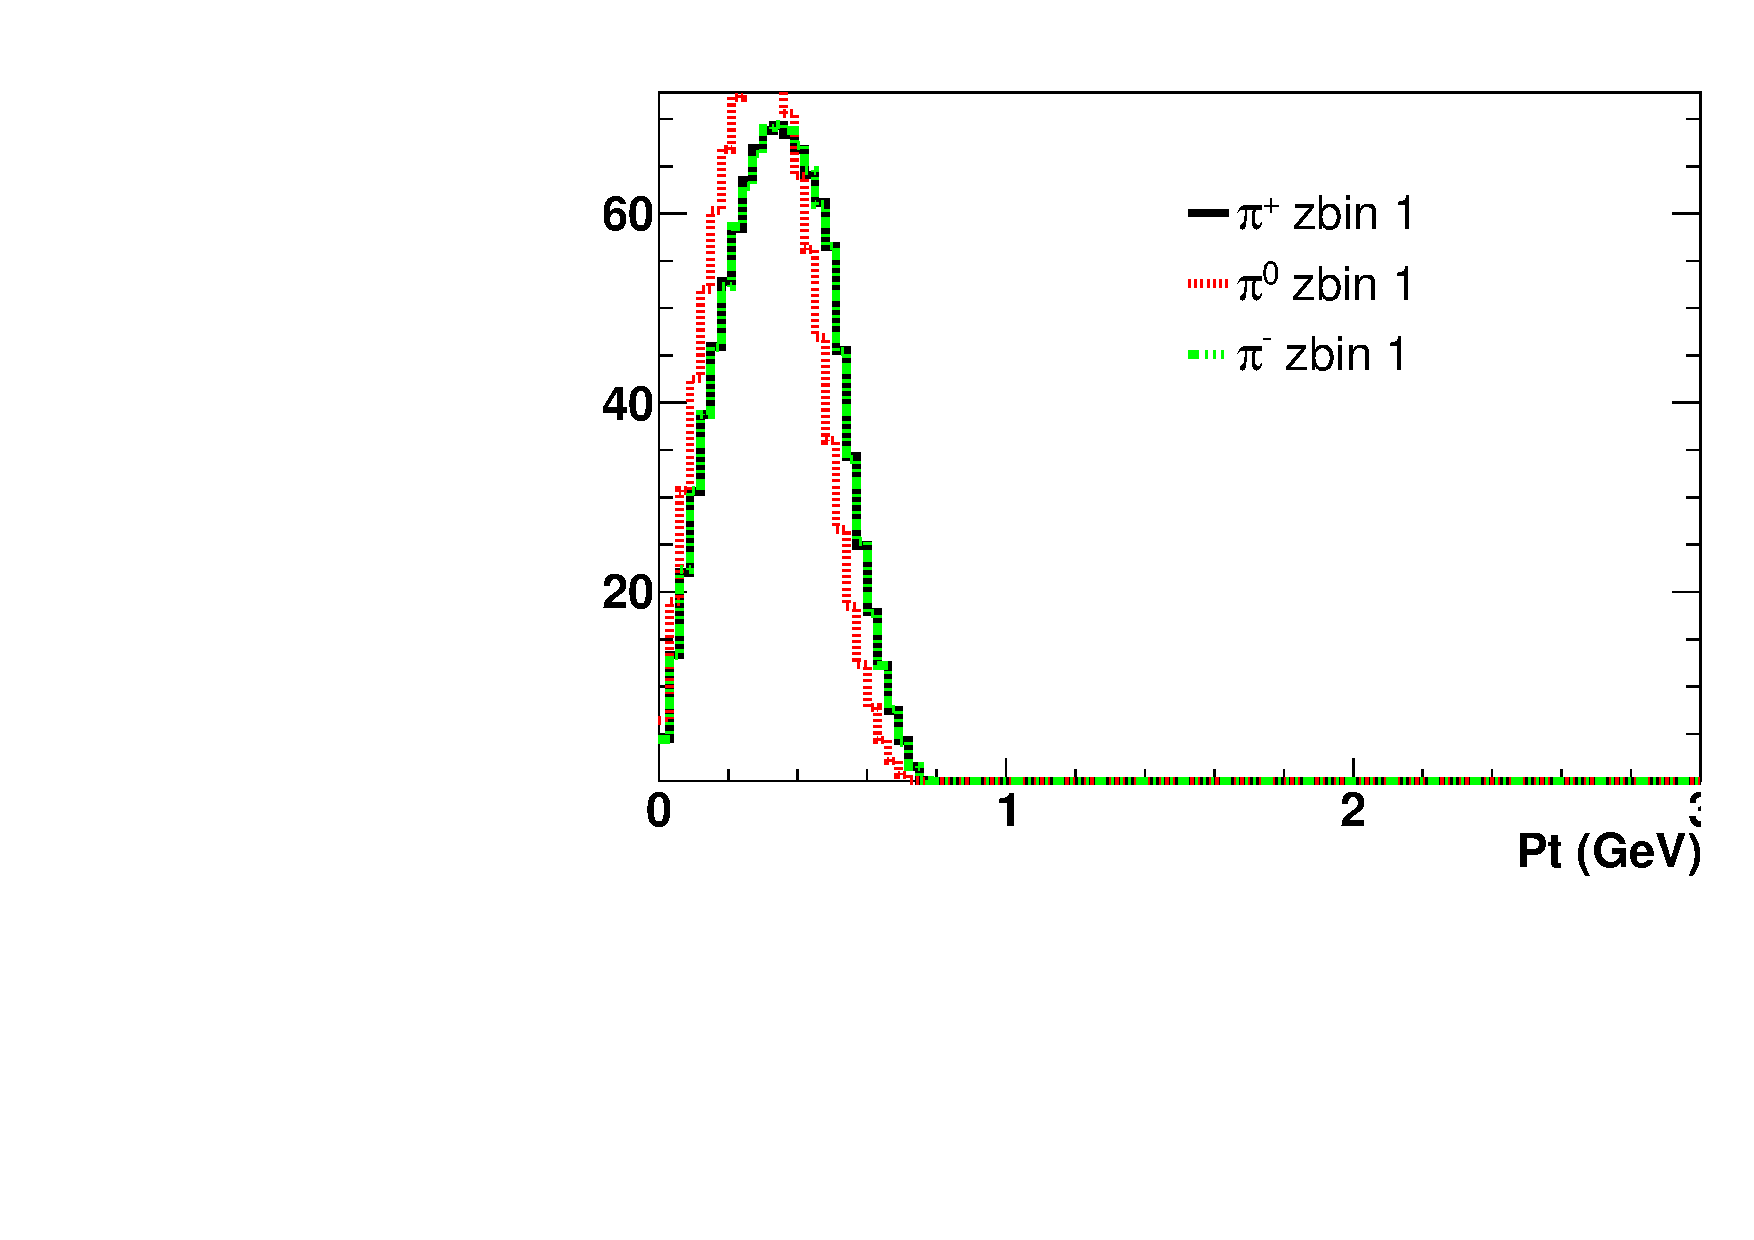
\includegraphics[width=.31\textwidth,natwidth=250,natheight=100]{figure_fiducial/had0.5/Pt_distri_for_zbin_1_norm_had05.pdf}\label{fig:kine_distri13}}
\caption{Normalized $P_t$ distributions of pions for $0.2<z<0.3$.}
\label{fig:kine_distri1}
\end{figure}

\begin{figure}[H]
\captionsetup[subfloat]{farskip=2pt,captionskip=1pt}
\centering
\subfigure[$H_{OA}<0.3$]{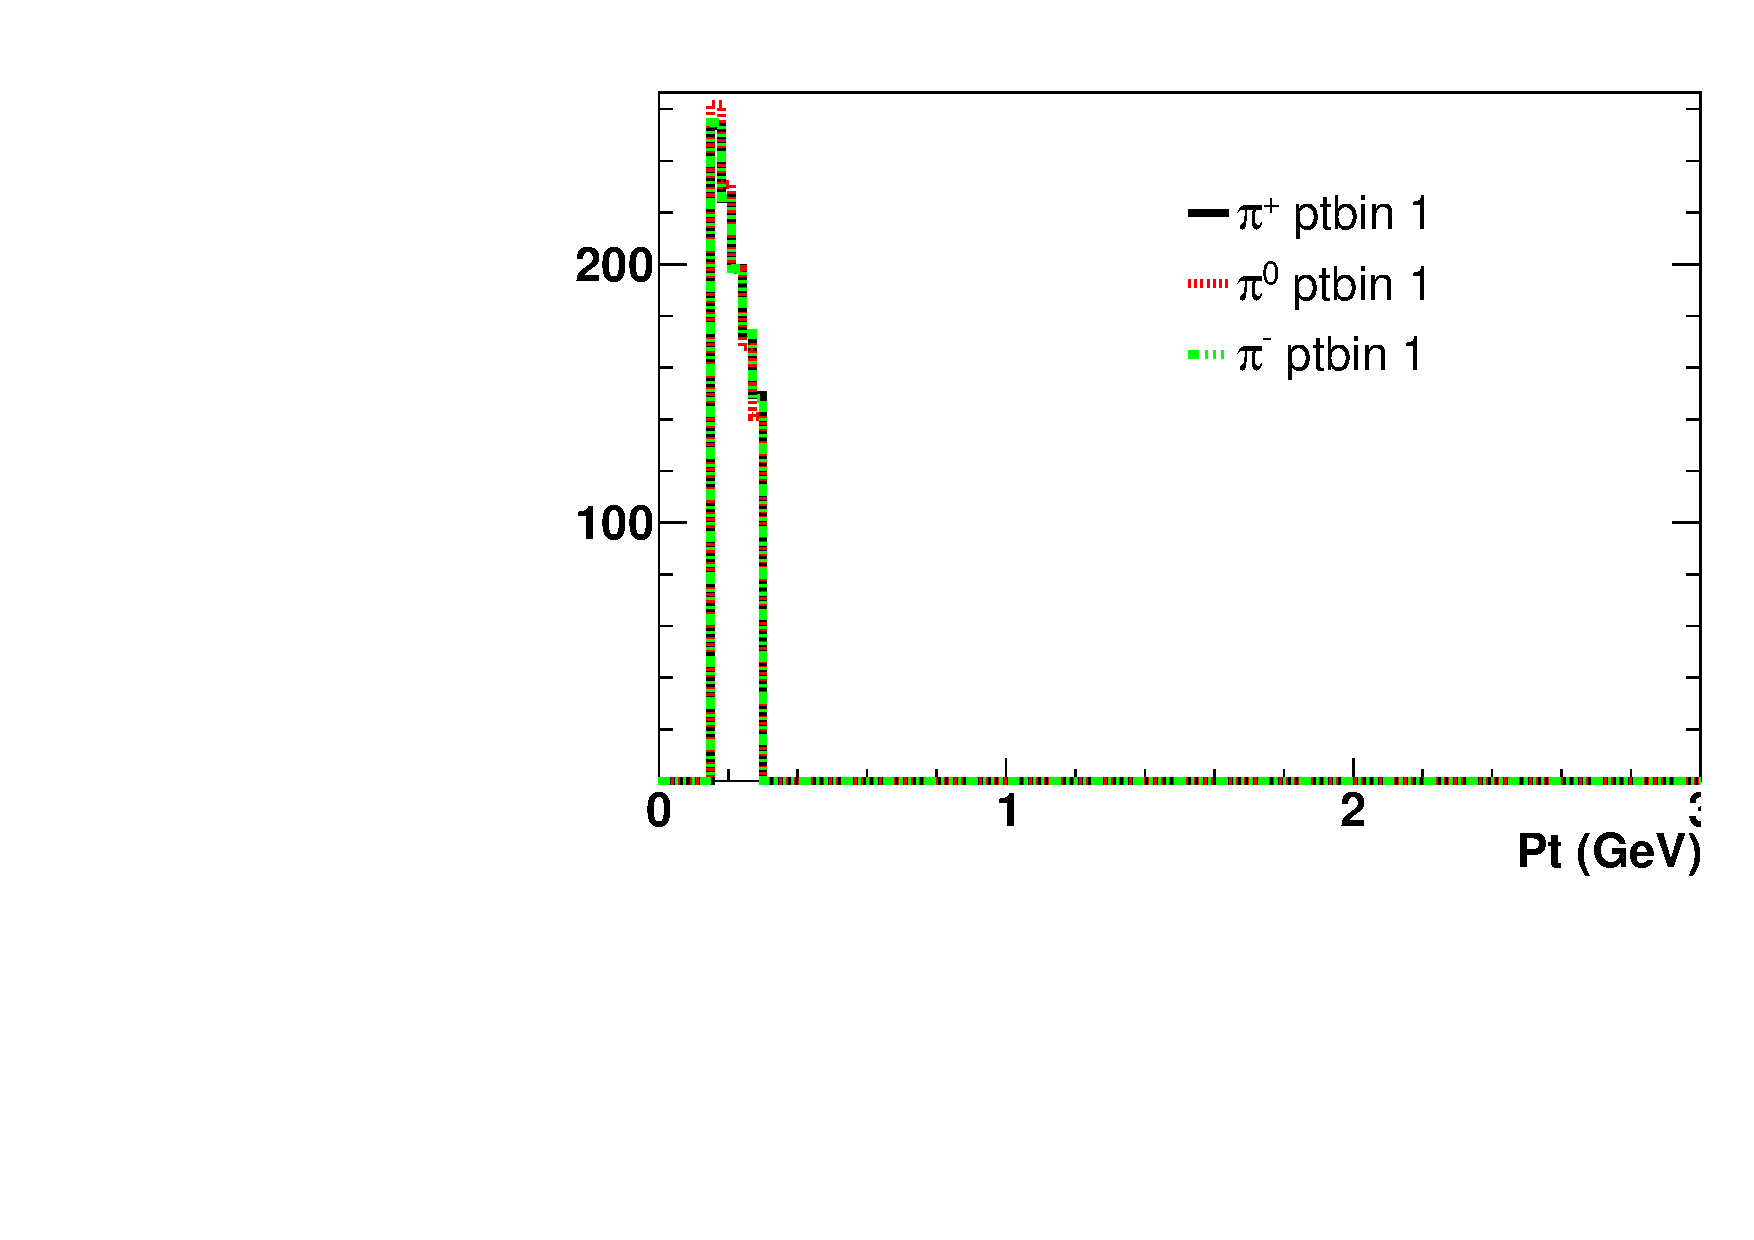
\includegraphics[width=.31\textwidth,natwidth=250,natheight=100]{figure_fiducial/had0.3/Pt_distri_for_ptbin_1_norm_had03.pdf}\label{fig:kine_distri21}}
\subfigure[$H_{OA}<0.4$]{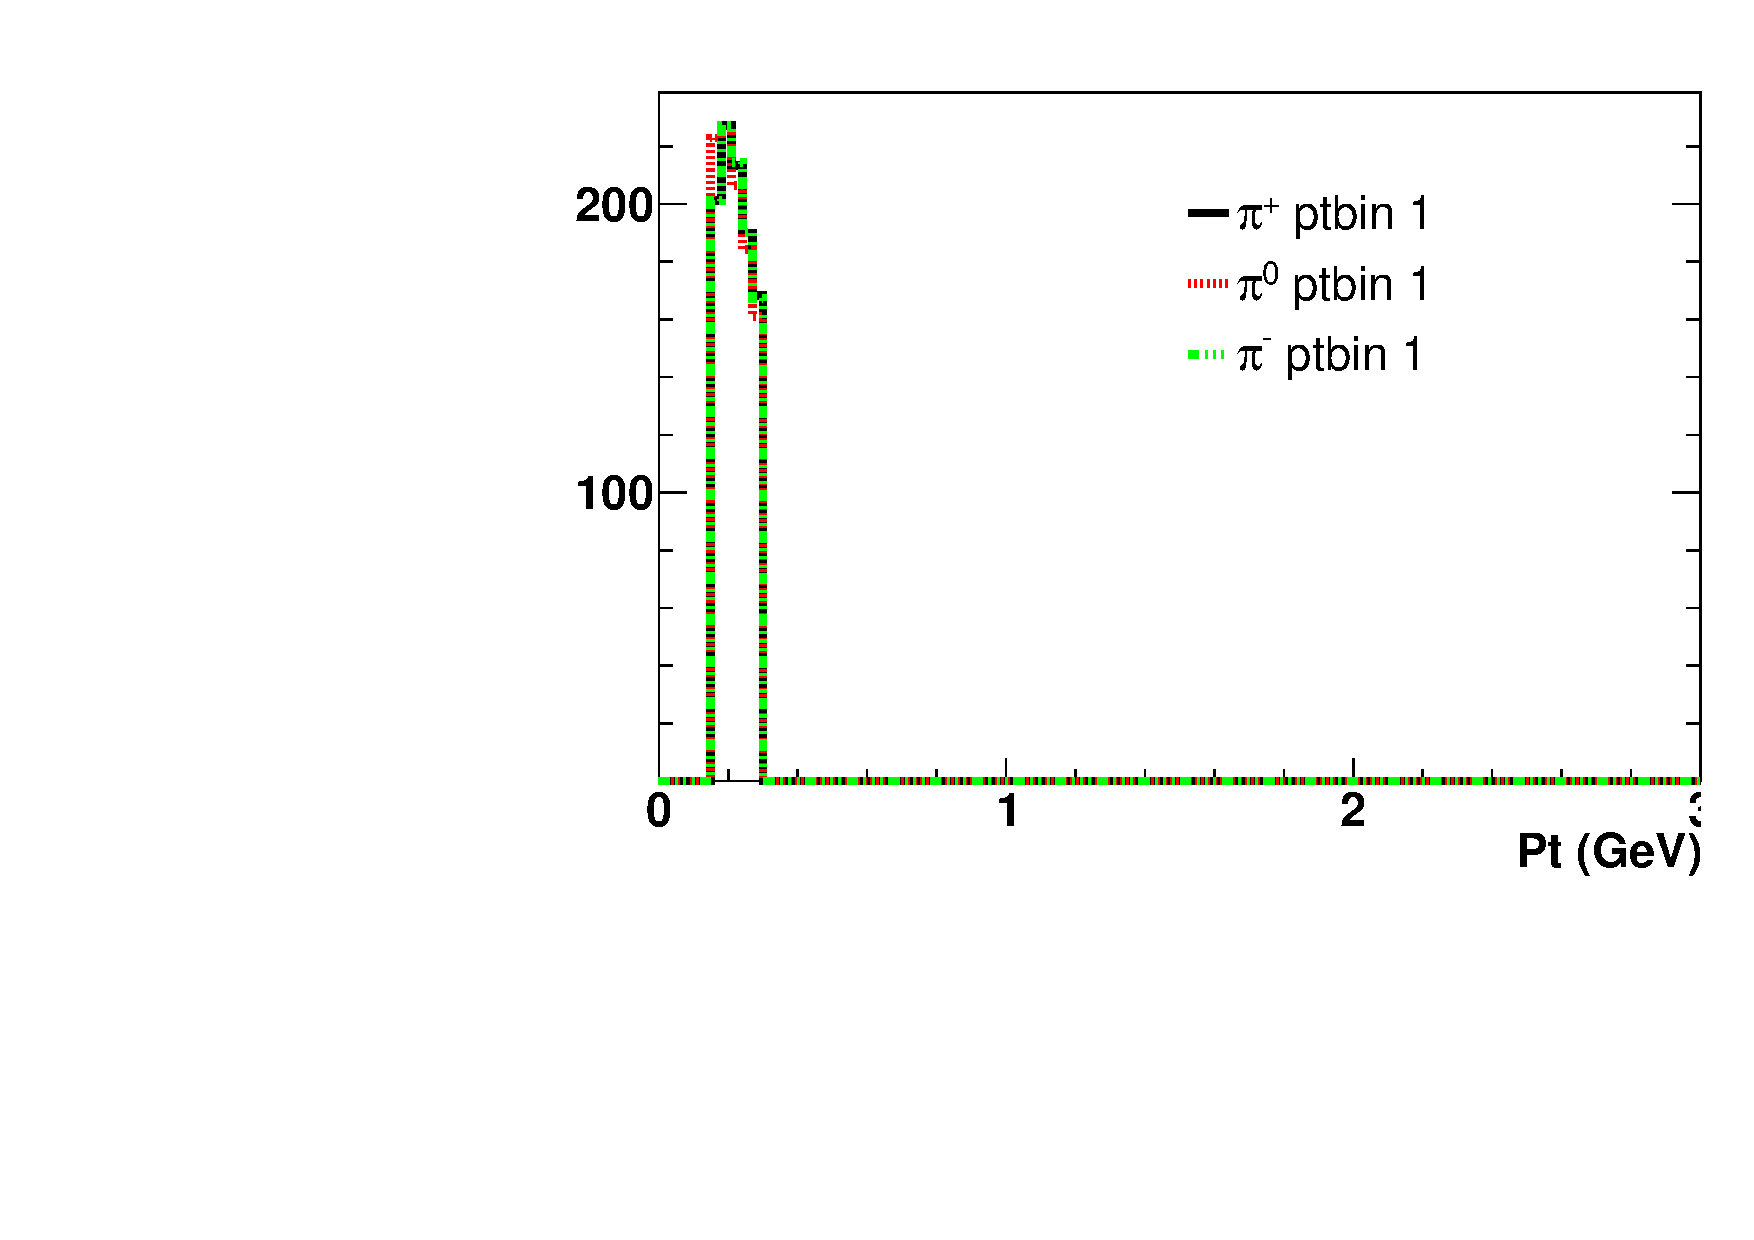
\includegraphics[width=.31\textwidth,natwidth=250,natheight=100]{figure_fiducial/had0.4/Pt_distri_for_ptbin_1_norm_had04.pdf}\label{fig:kine_distri22}}
\subfigure[$H_{OA}<0.5$]{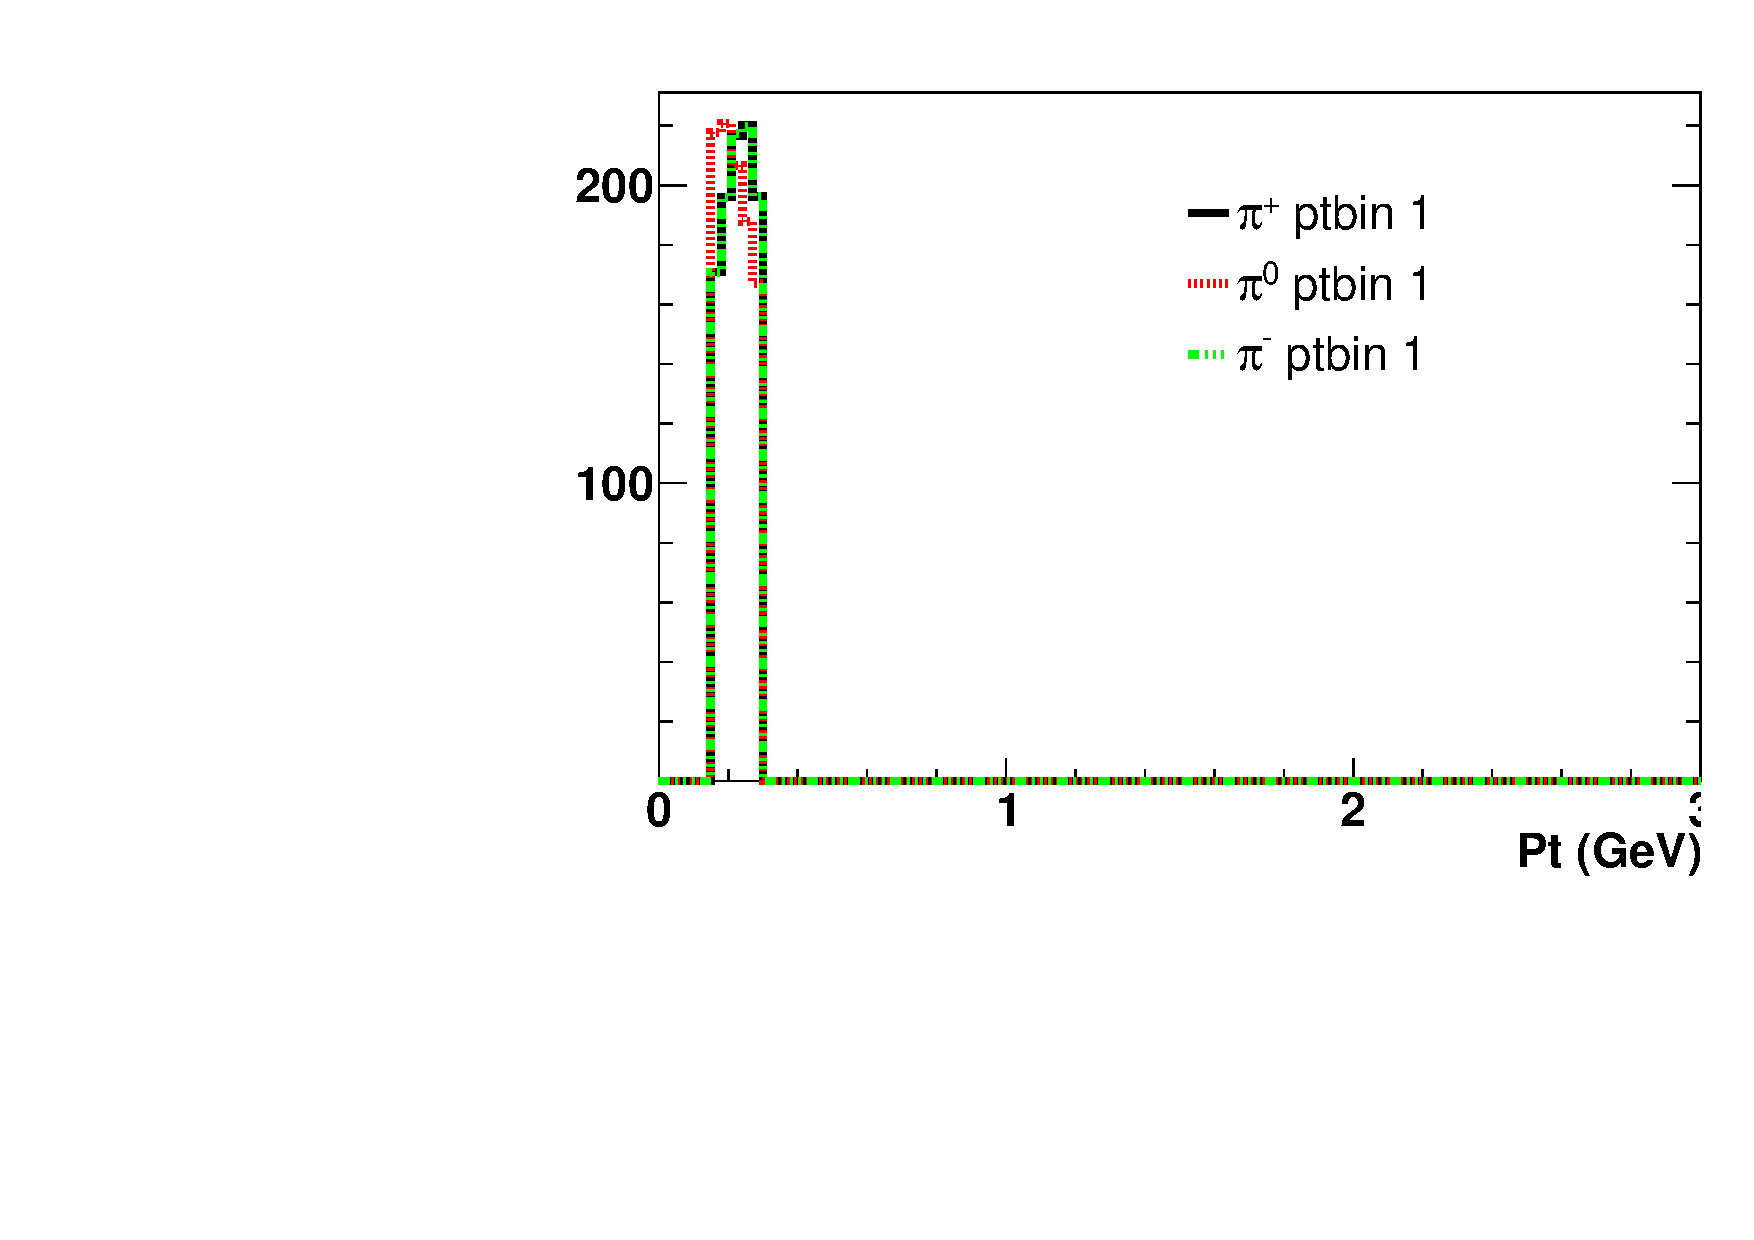
\includegraphics[width=.31\textwidth,natwidth=250,natheight=100]{figure_fiducial/had0.5/Pt_distri_for_ptbin_1_norm_had05.pdf}\label{fig:kine_distri23}}
\caption{Normalized $P_t$ distributions of pions for $P_{t}<0.15$~GeV.}
\label{fig:kine_distri2}
\end{figure}

\begin{figure}[H]
\captionsetup[subfloat]{farskip=2pt,captionskip=1pt}
\centering
\subfigure[$H_{OA}<0.3$]{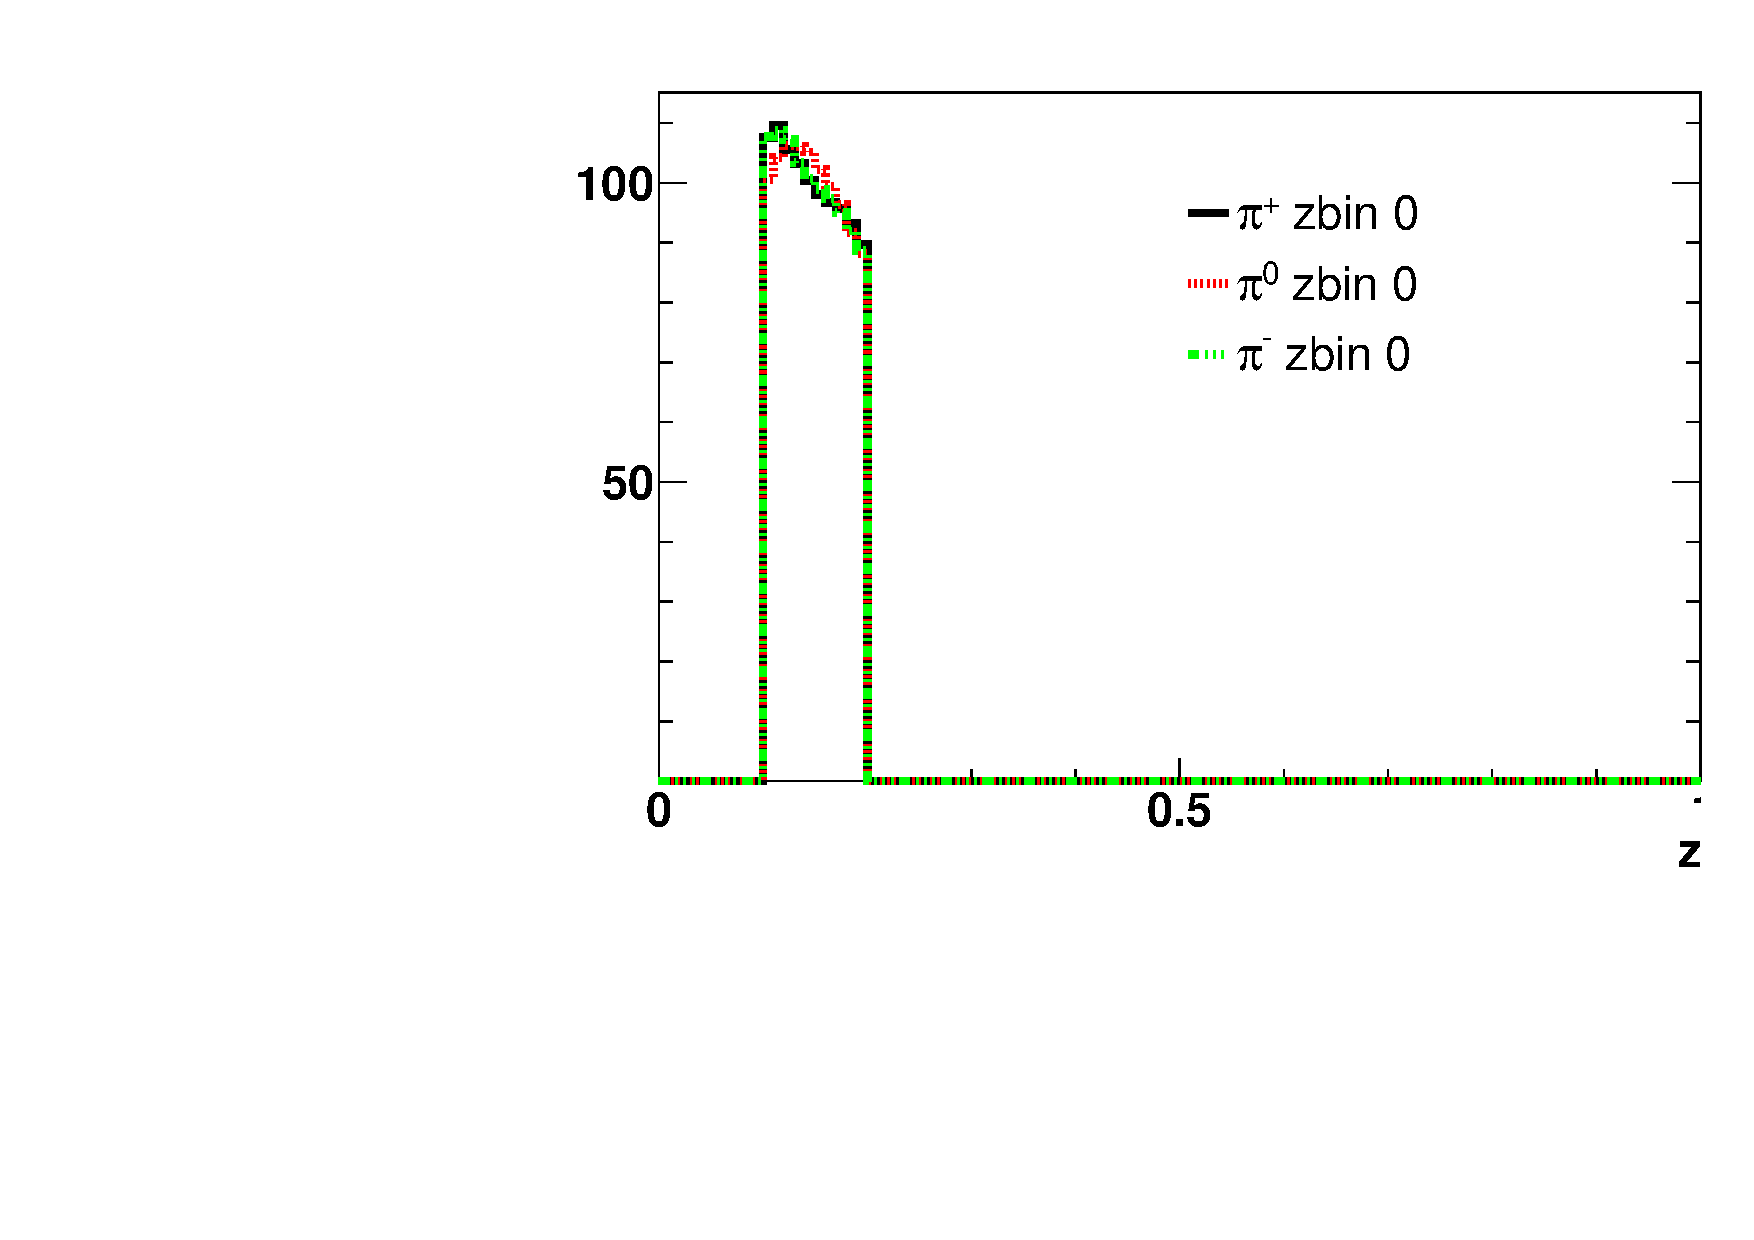
\includegraphics[width=.31\textwidth,natwidth=250,natheight=100]{figure_fiducial/had0.3/Z_distri_for_zbin_0_norm_had03.pdf}\label{fig:kine_distri31}}
\subfigure[$H_{OA}<0.4$]{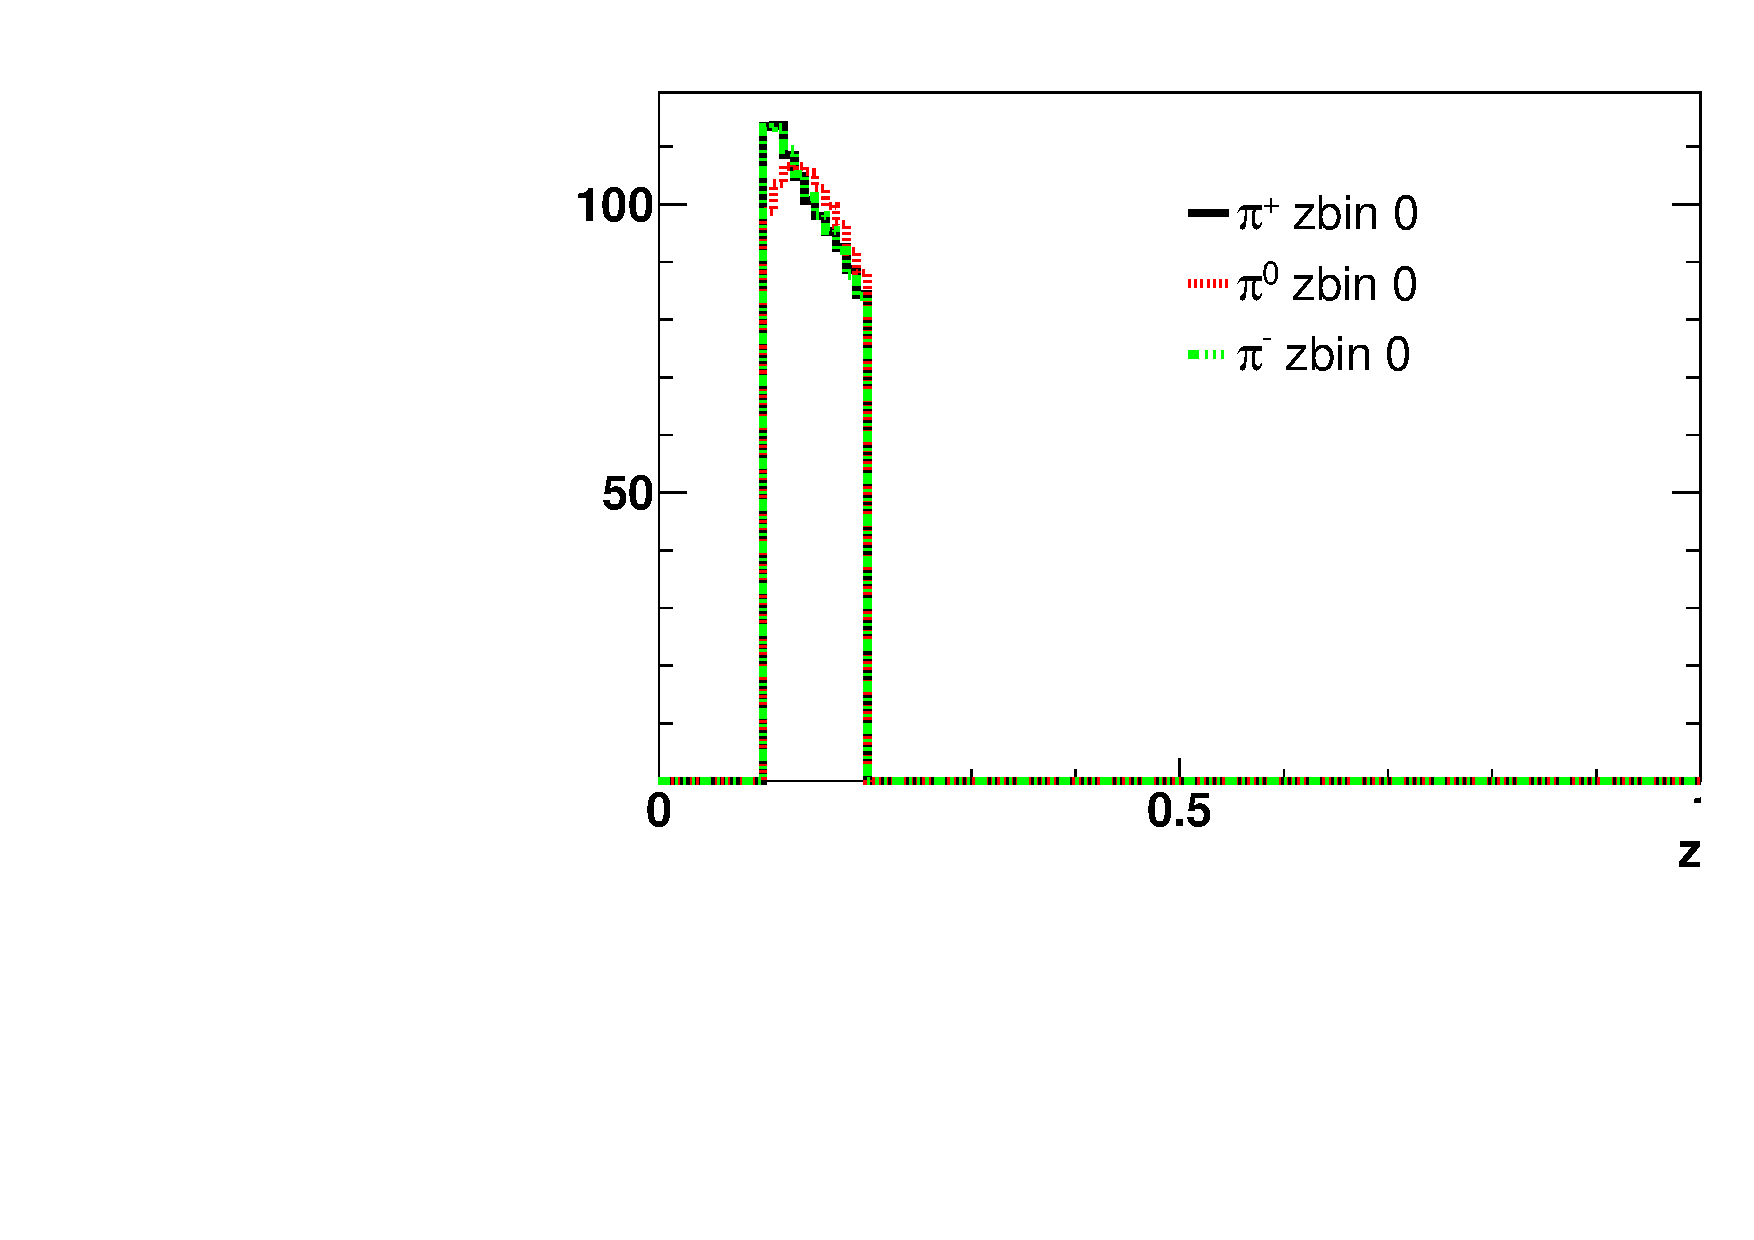
\includegraphics[width=.31\textwidth,natwidth=250,natheight=100]{figure_fiducial/had0.4/Z_distri_for_zbin_0_norm_had04.pdf}\label{fig:kine_distri32}}
\subfigure[$H_{OA}<0.5$]{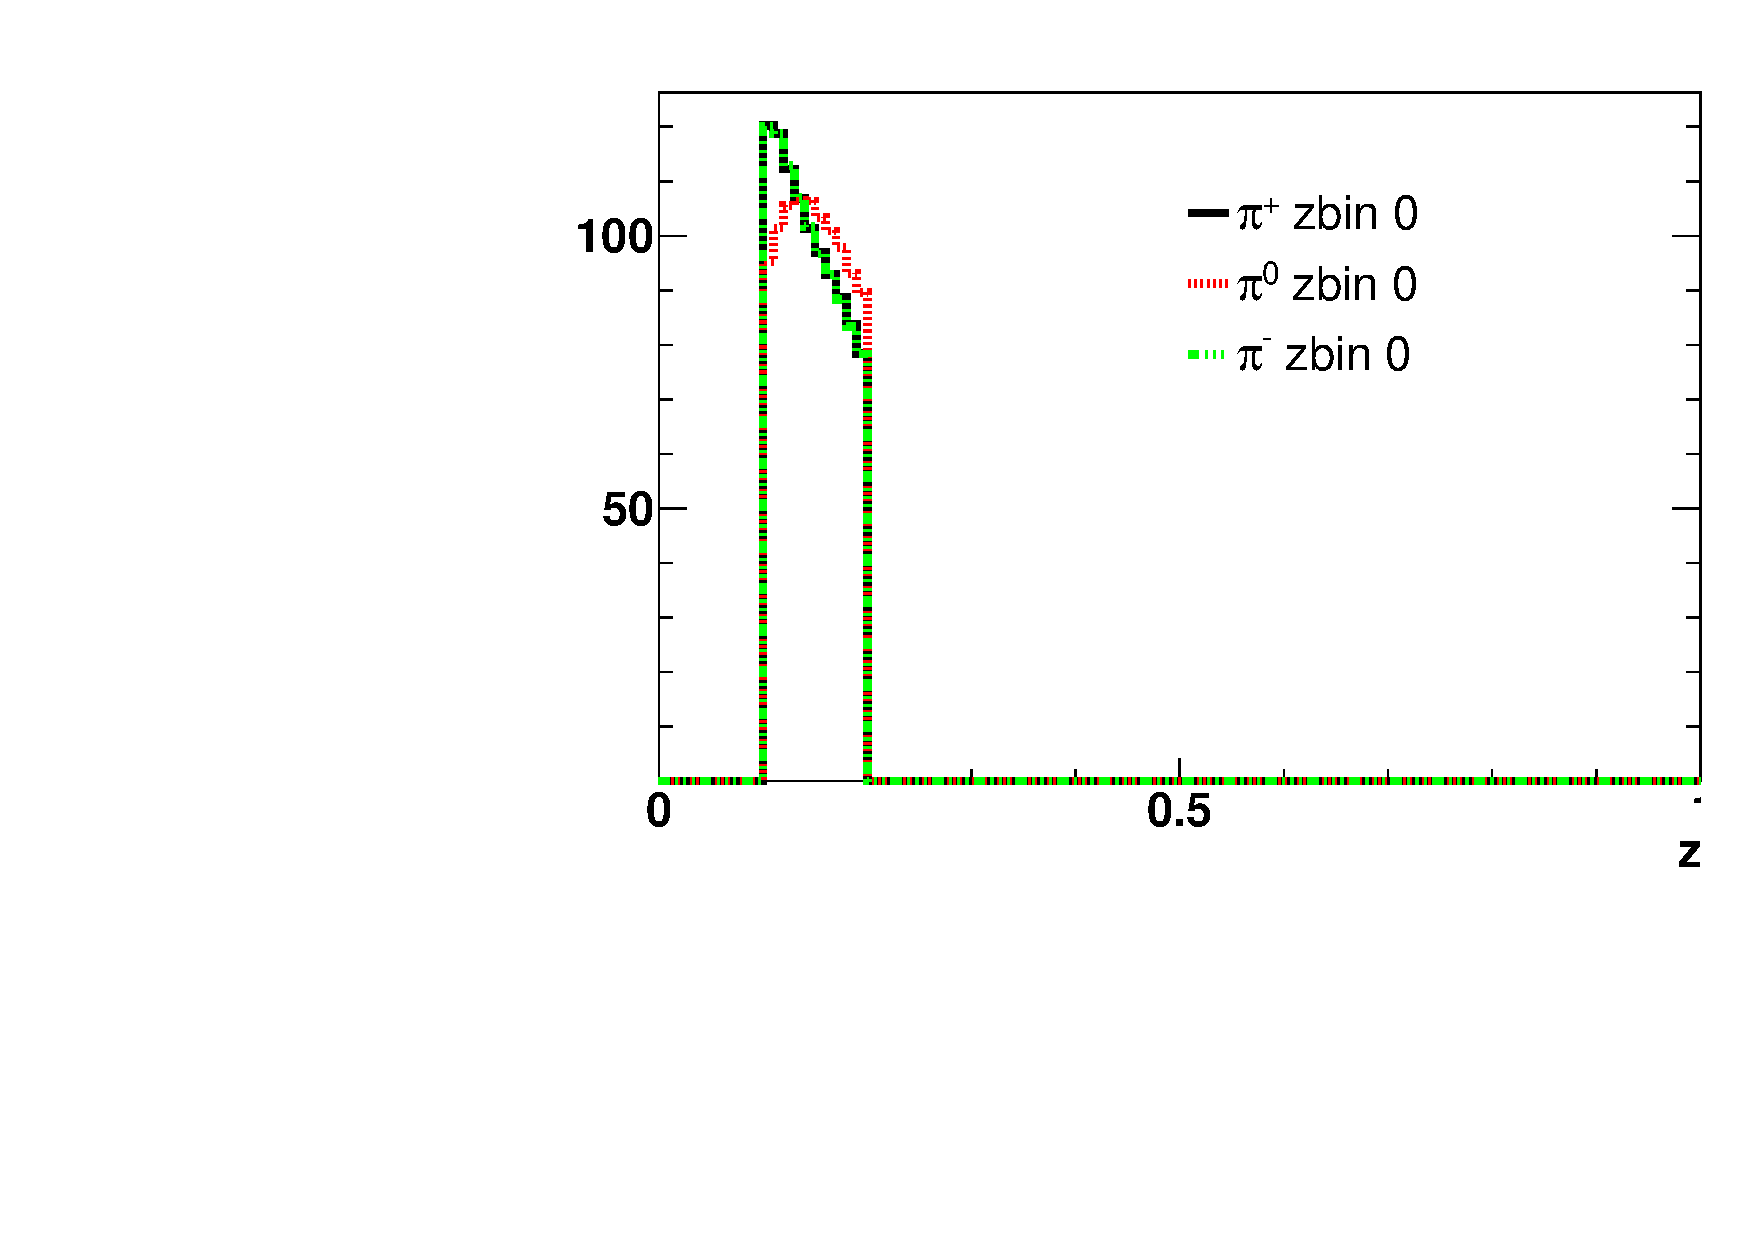
\includegraphics[width=.31\textwidth,natwidth=250,natheight=100]{figure_fiducial/had0.5/Z_distri_for_zbin_0_norm_had05.pdf}\label{fig:kine_distri33}}
\caption{Normalized $z$ distributions of pions for $0.1<z<0.2$.}
\label{fig:kine_distri3}
\end{figure}

\begin{figure}[H]
\captionsetup[subfloat]{farskip=2pt,captionskip=1pt}
\centering
\subfigure[$H_{OA}<0.3$]{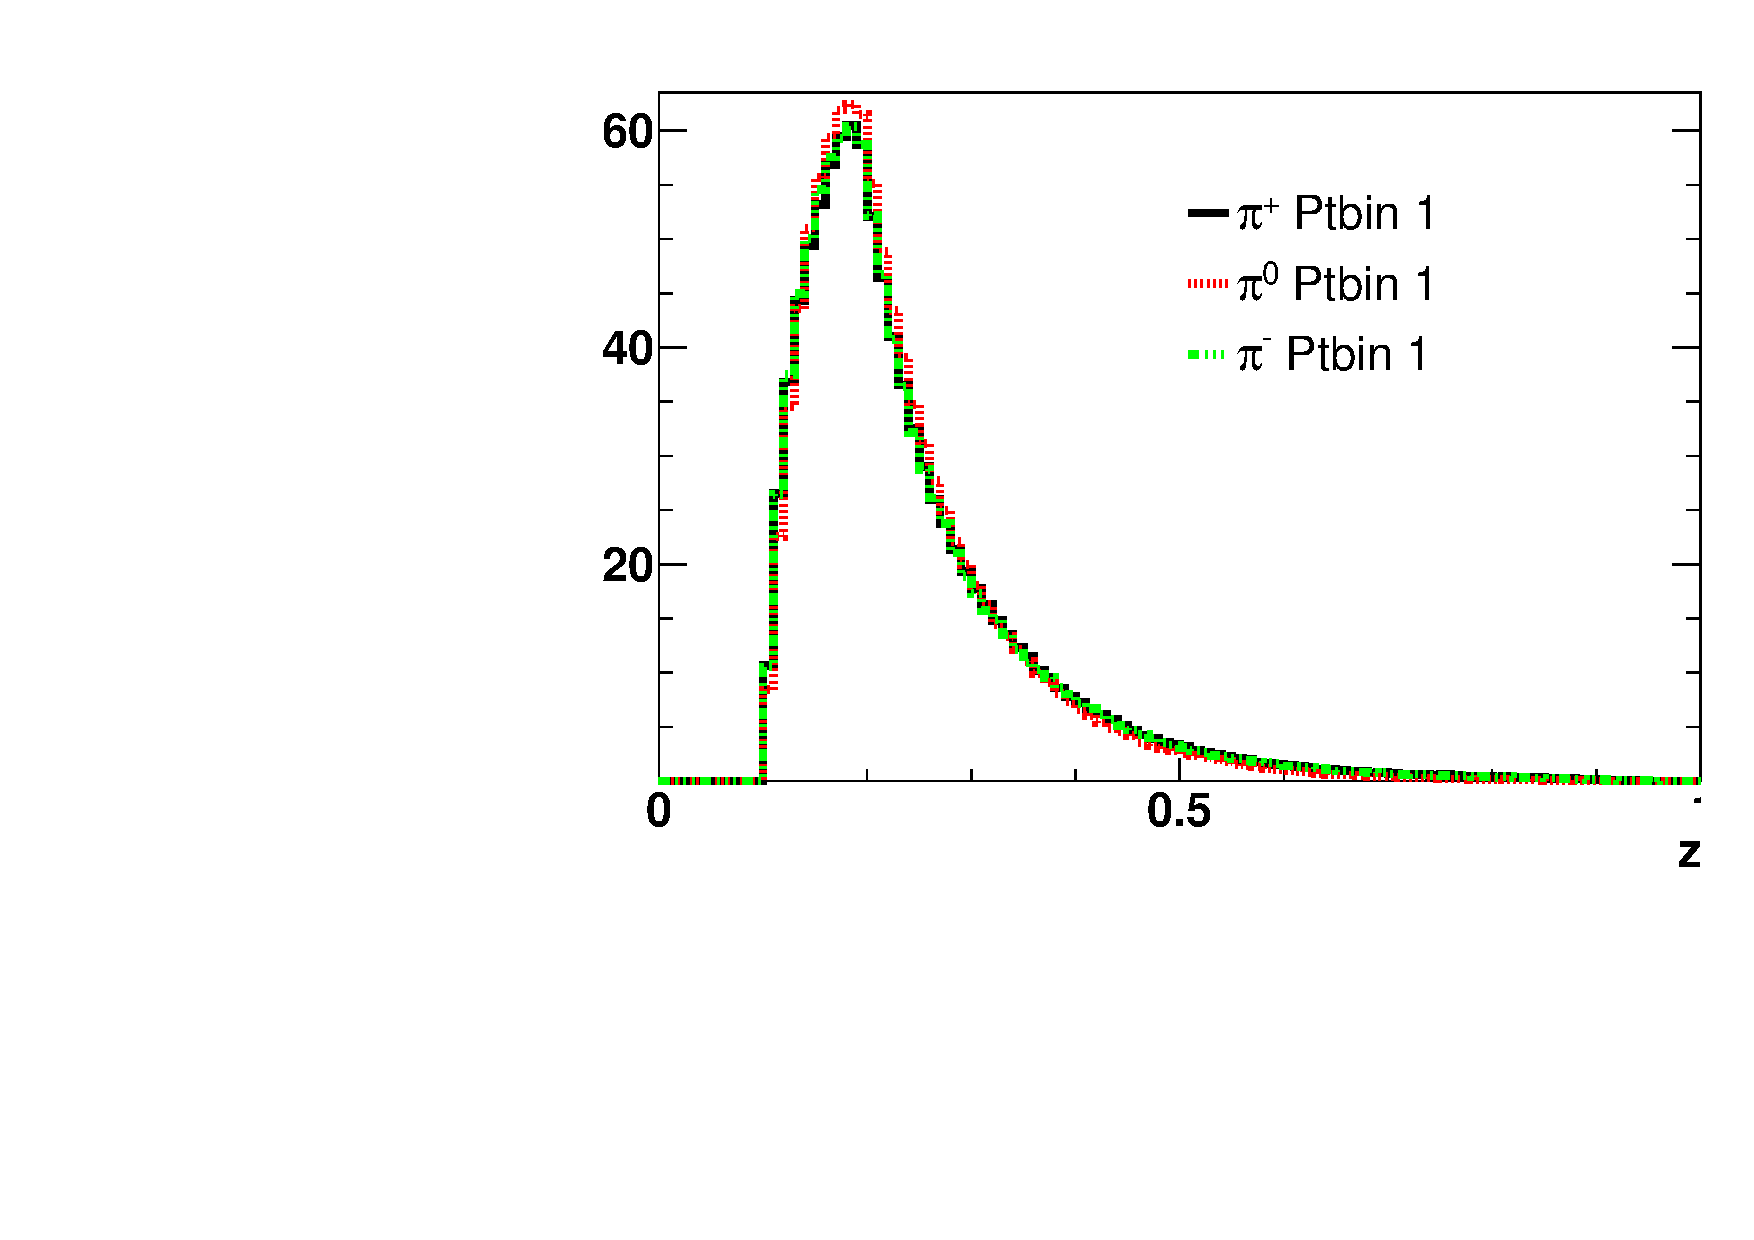
\includegraphics[width=.31\textwidth,natwidth=250,natheight=100]{figure_fiducial/had0.3/Z_distri_for_ptbin_1_norm_had03.pdf}\label{fig:kine_distri41}}
\subfigure[$H_{OA}<0.4$]{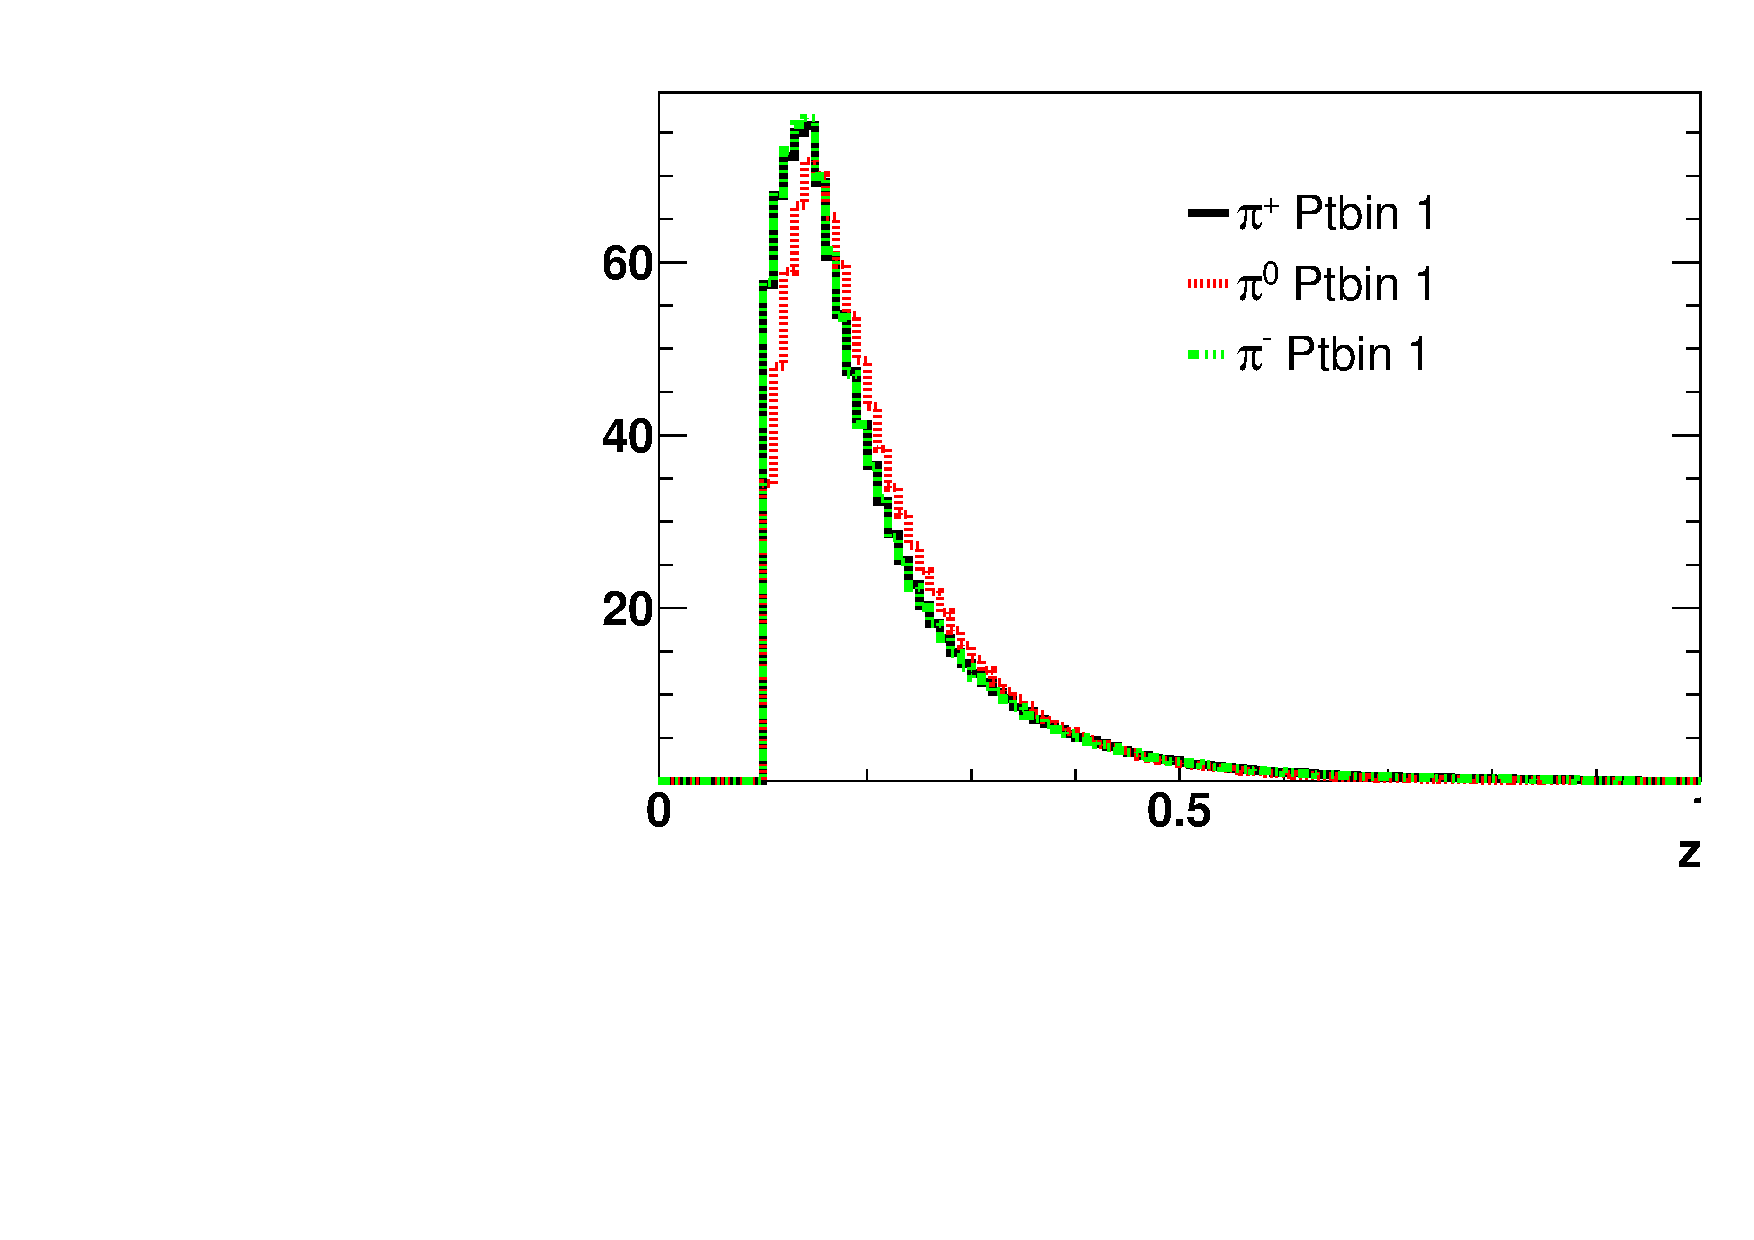
\includegraphics[width=.31\textwidth,natwidth=250,natheight=100]{figure_fiducial/had0.4/Z_distri_for_ptbin_1_norm_had04.pdf}\label{fig:kine_distri42}}
\subfigure[$H_{OA}<0.5$]{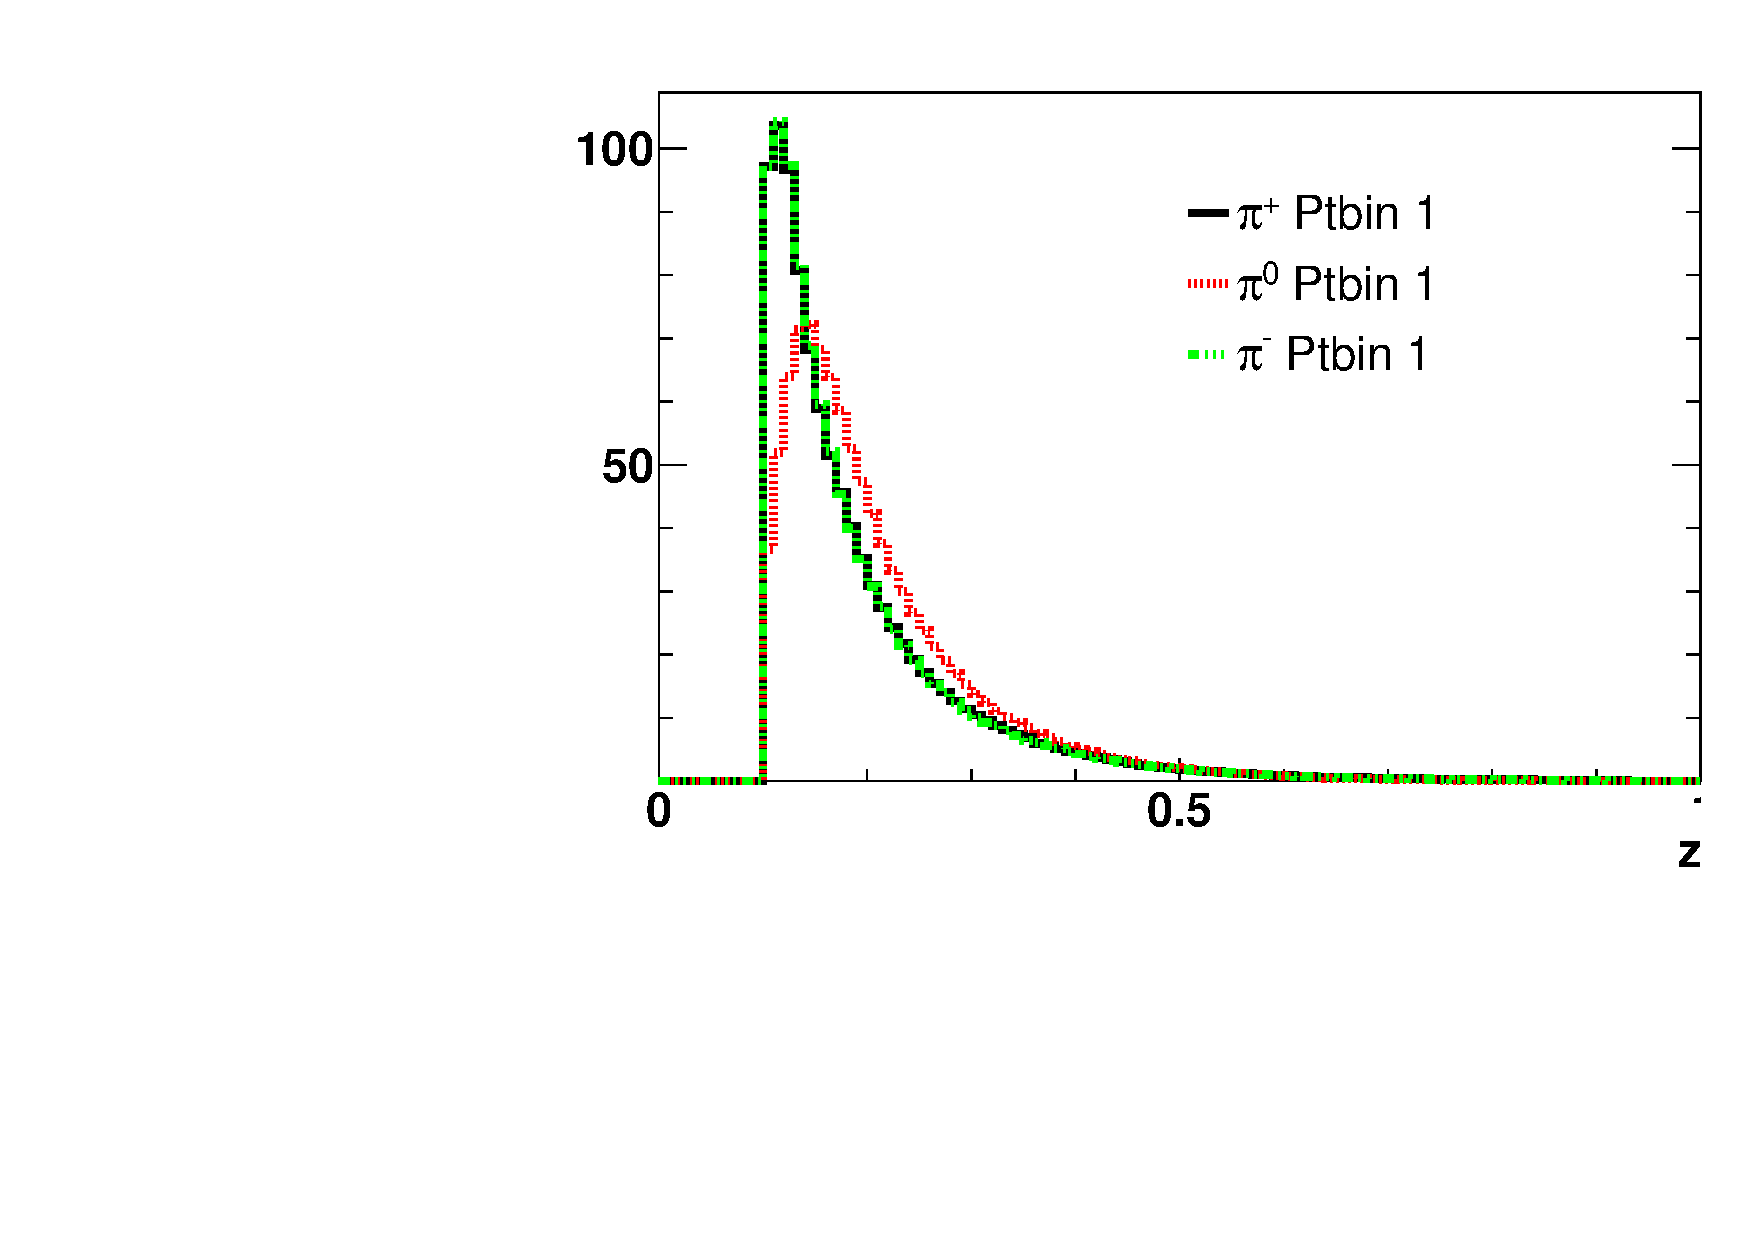
\includegraphics[width=.31\textwidth,natwidth=250,natheight=100]{figure_fiducial/had0.5/Z_distri_for_ptbin_1_norm_had05.pdf}\label{fig:kine_distri43}}
\caption{Normalized $z$ distributions of pions for 0.15~GeV $<P_t<0.3$~GeV.}
\label{fig:kine_distri4}
\end{figure}

\begin{figure}[H]
\captionsetup[subfloat]{farskip=2pt,captionskip=1pt}
\centering
\subfigure[$H_{OA}<0.3$]{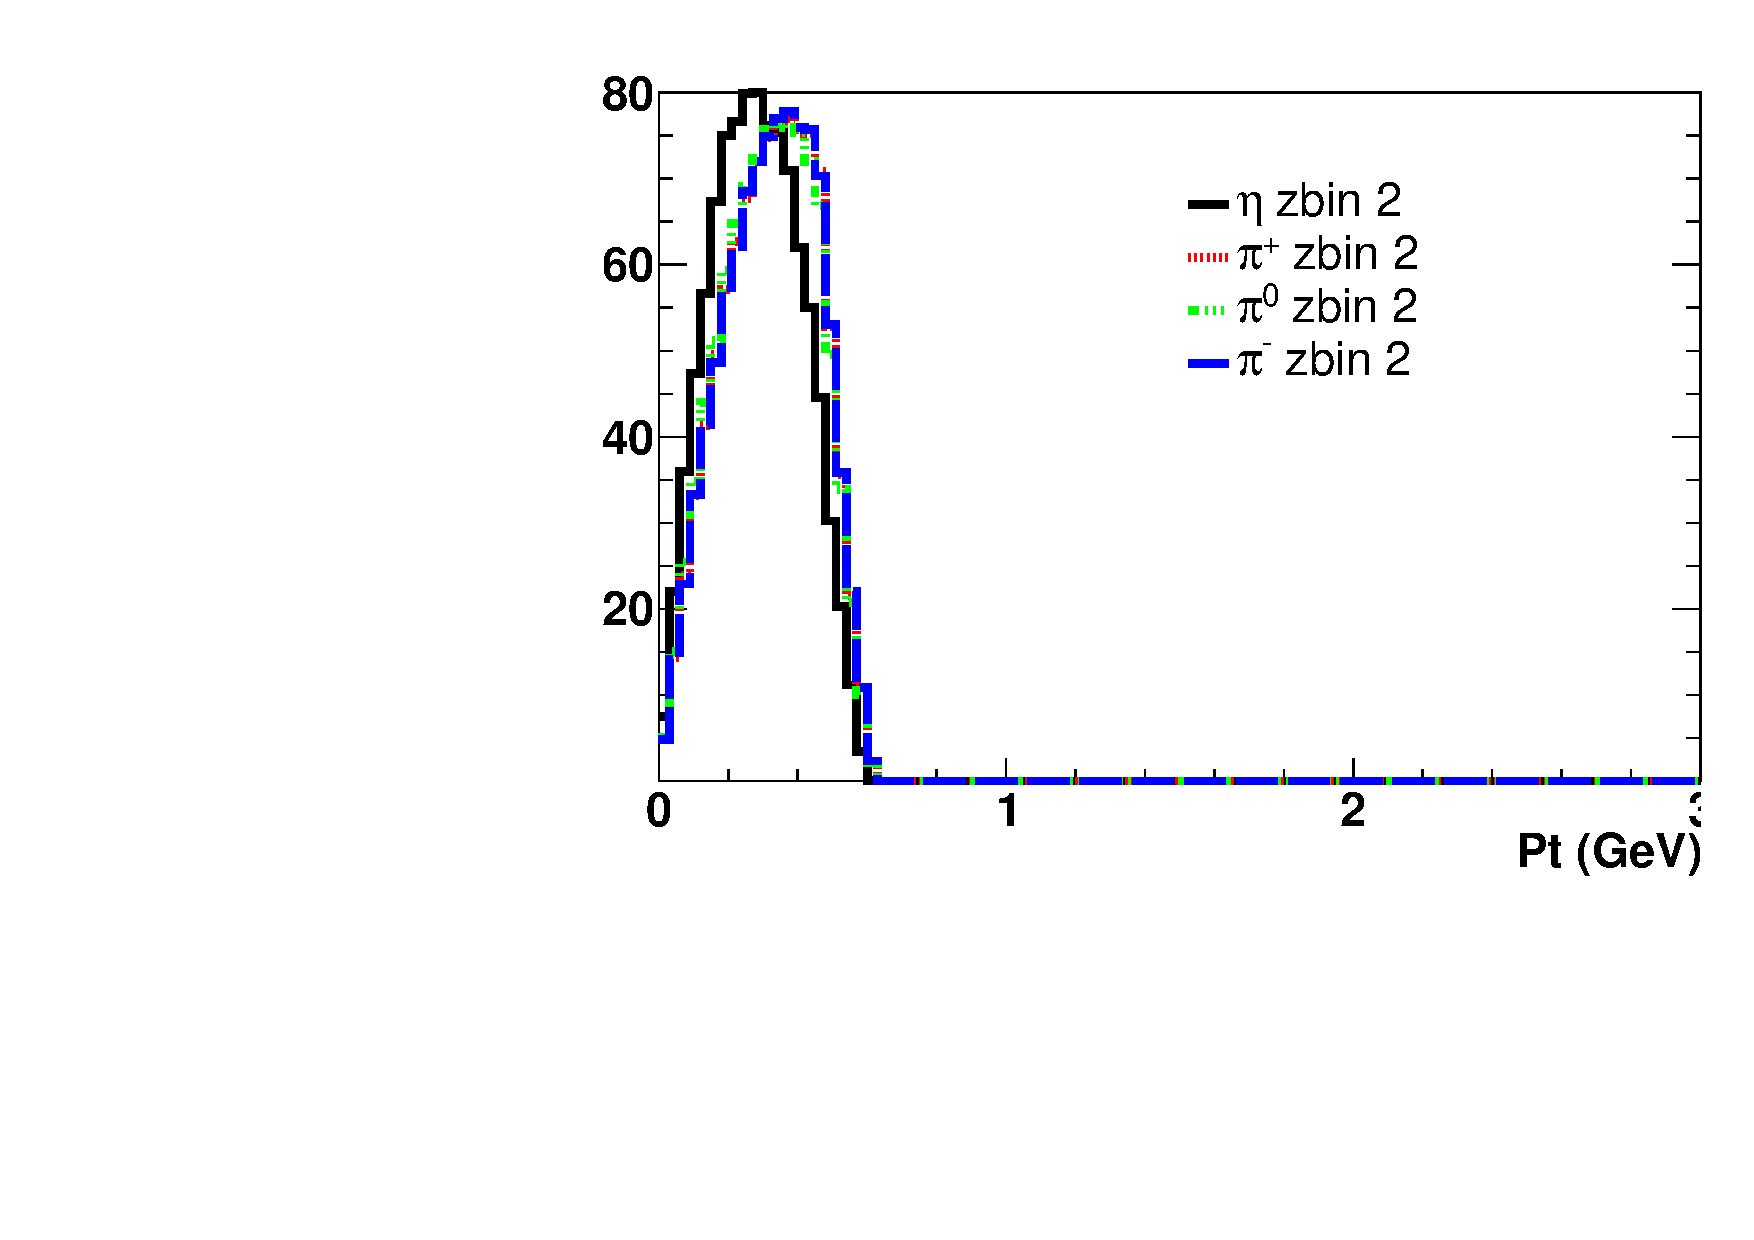
\includegraphics[width=.31\textwidth,natwidth=250,natheight=100]{figure_fiducial/had0.3_z0.3/Pt_distri_for_zbin_2_norm_had03z03.pdf}\label{fig:kine_distri51}}
\subfigure[$H_{OA}<0.4$]{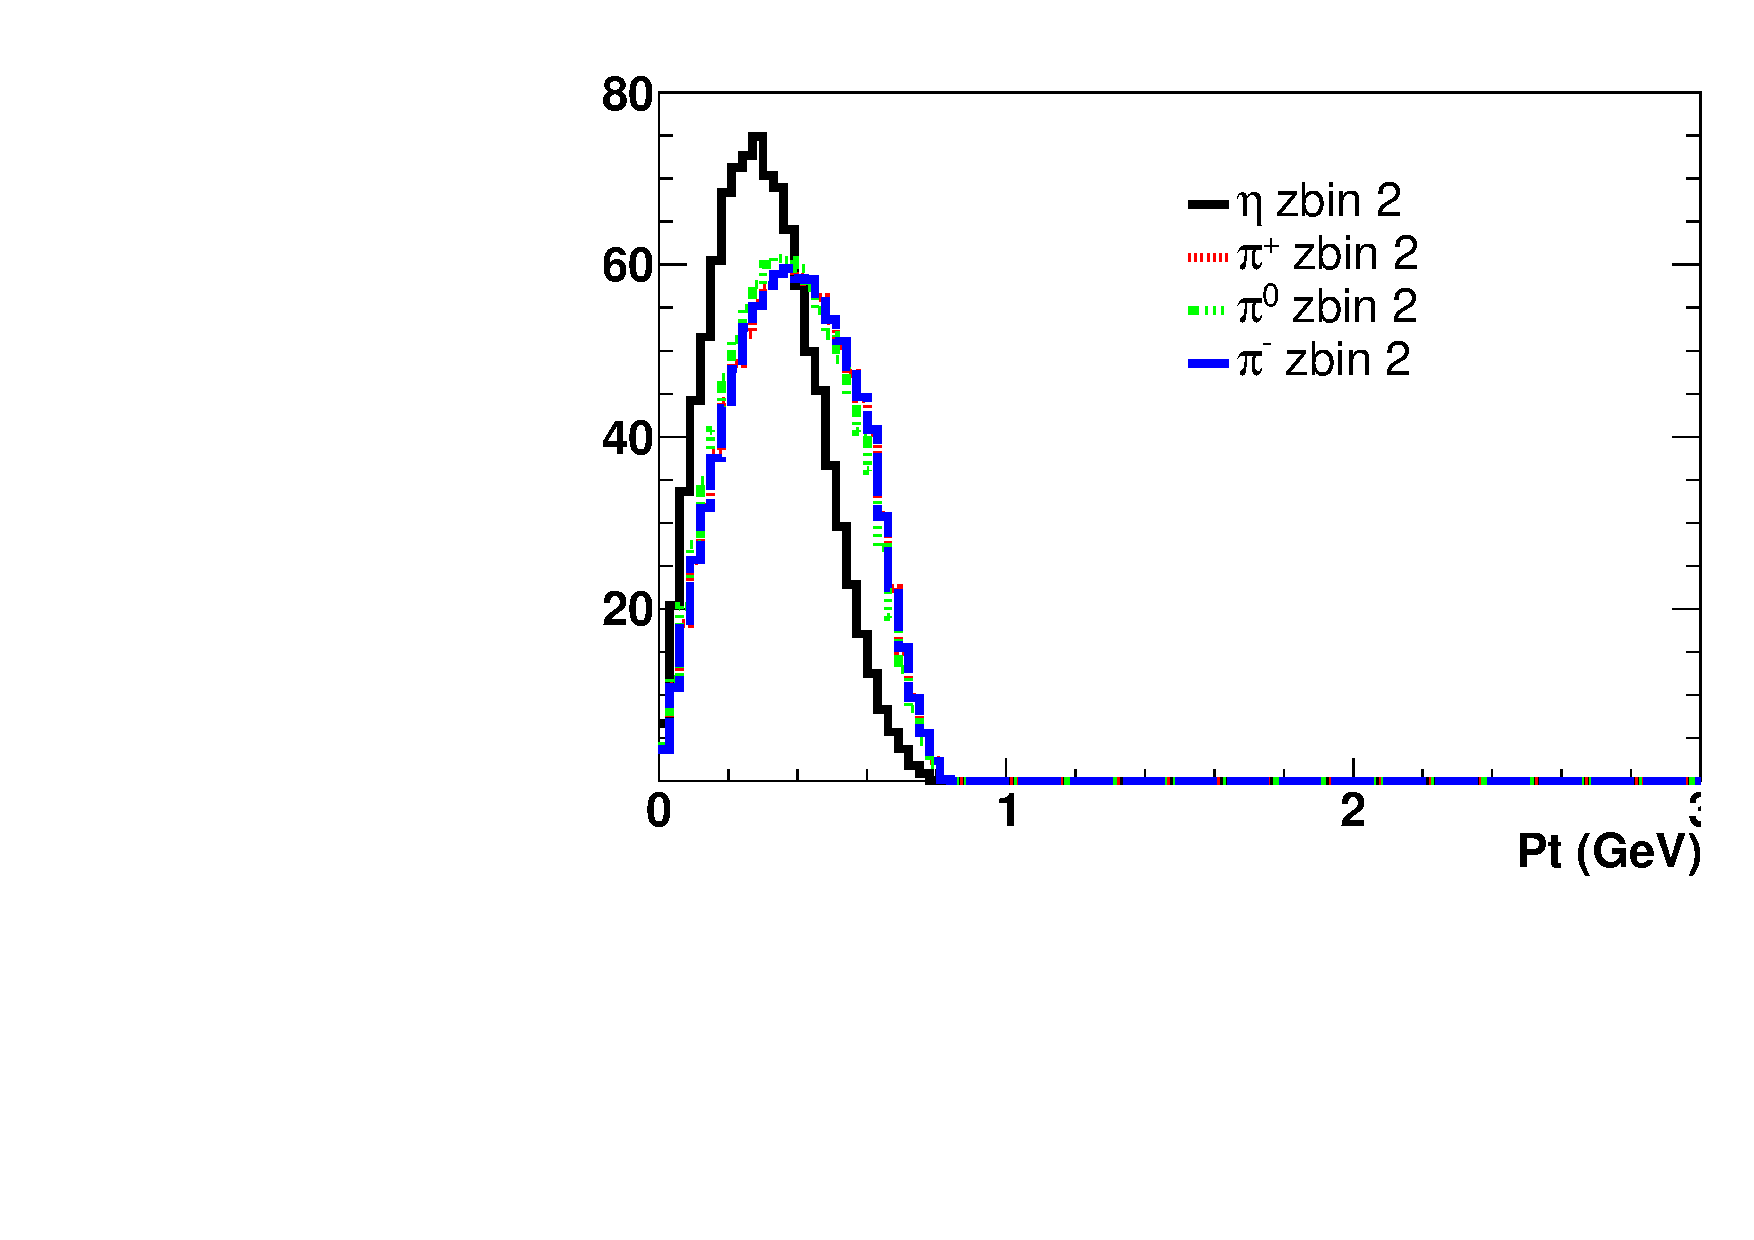
\includegraphics[width=.31\textwidth,natwidth=250,natheight=100]{figure_fiducial/had0.4_z0.3/Pt_distri_for_zbin_2_norm_had04z03.pdf}\label{fig:kine_distri52}}
\caption{Normalized $P_t$ distributions of $\eta$ and pions for $0.3<z<0.4$.}
\label{fig:kine_distri5}
\end{figure}

\begin{figure}[H]
\captionsetup[subfloat]{farskip=2pt,captionskip=1pt}
\centering
\subfigure[$H_{OA}<0.3$]{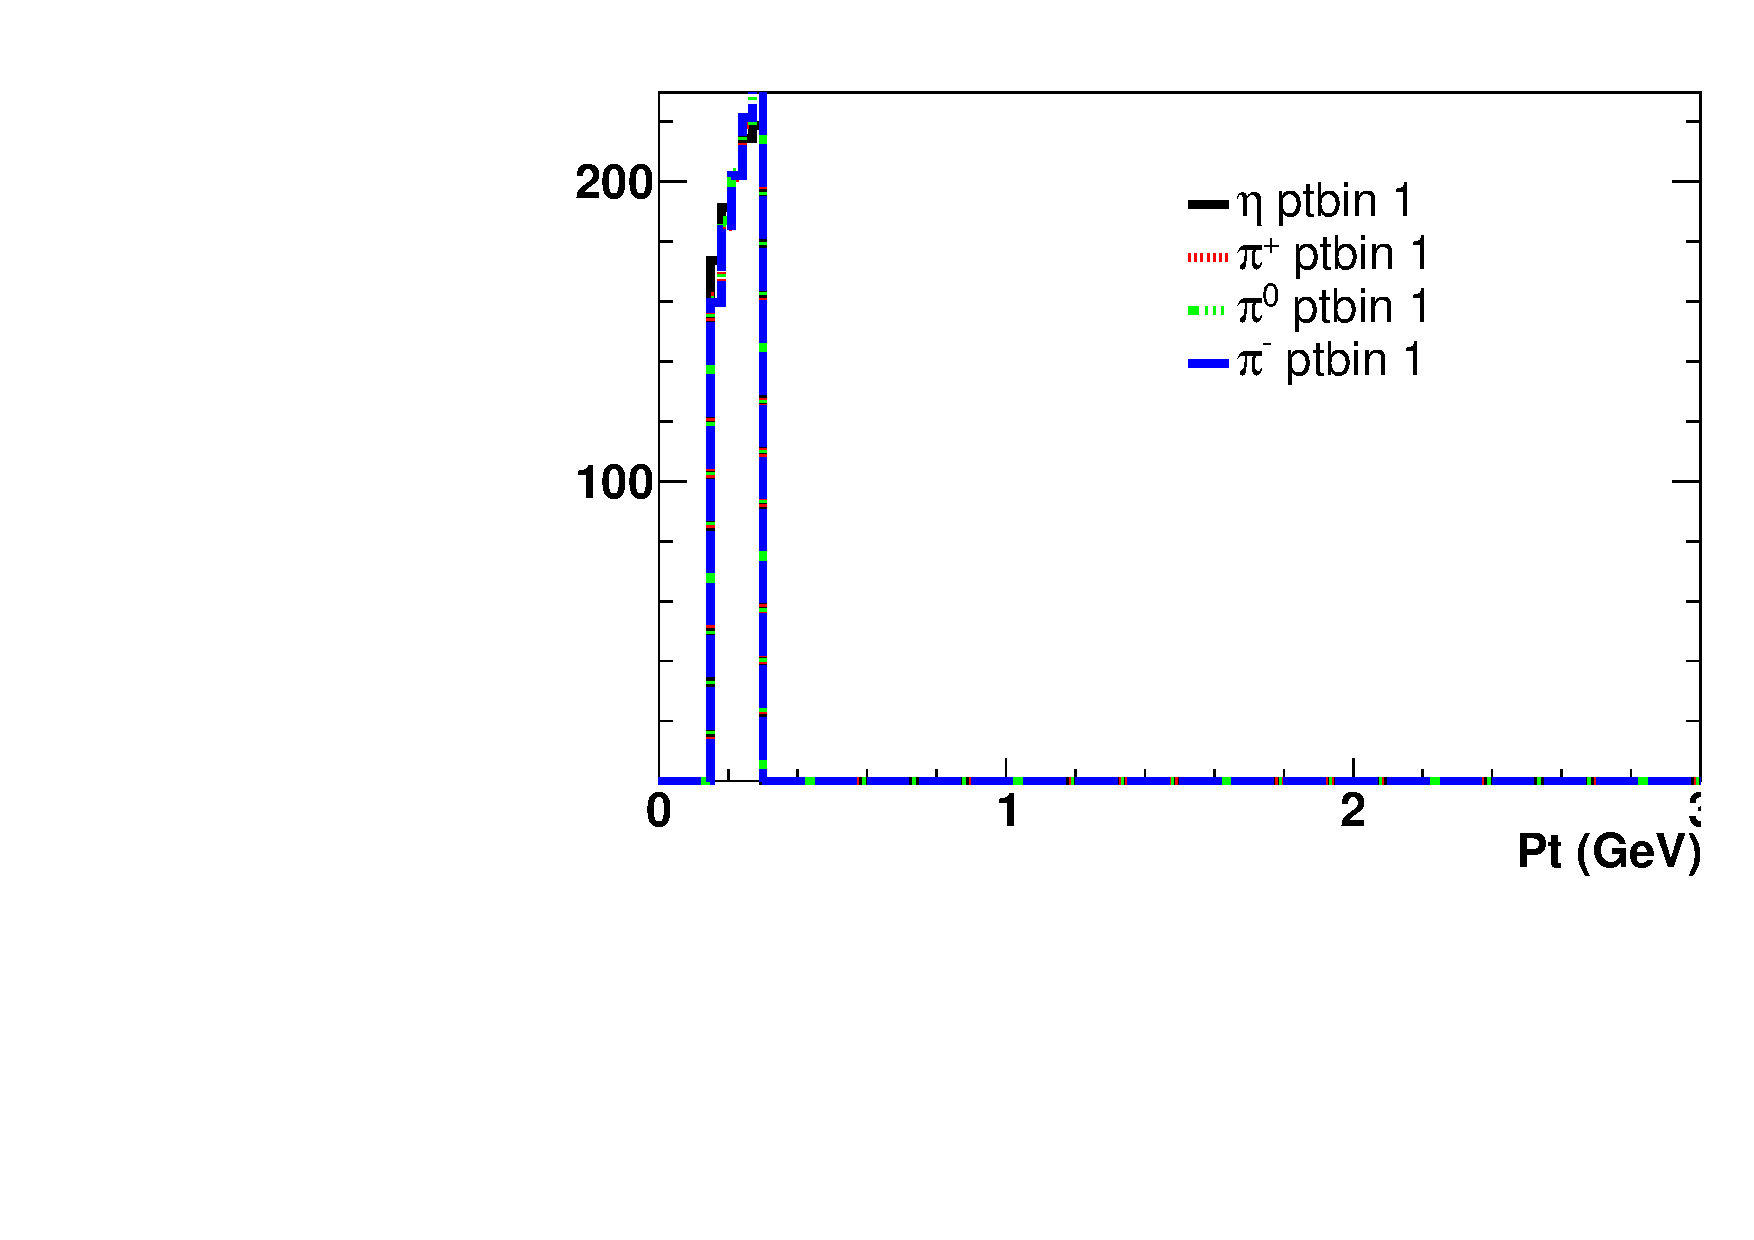
\includegraphics[width=.31\textwidth,natwidth=250,natheight=100]{figure_fiducial/had0.3_z0.3/Pt_distri_for_ptbin_1_norm_had03z03.pdf}\label{fig:kine_distri61}}
\subfigure[$H_{OA}<0.4$]{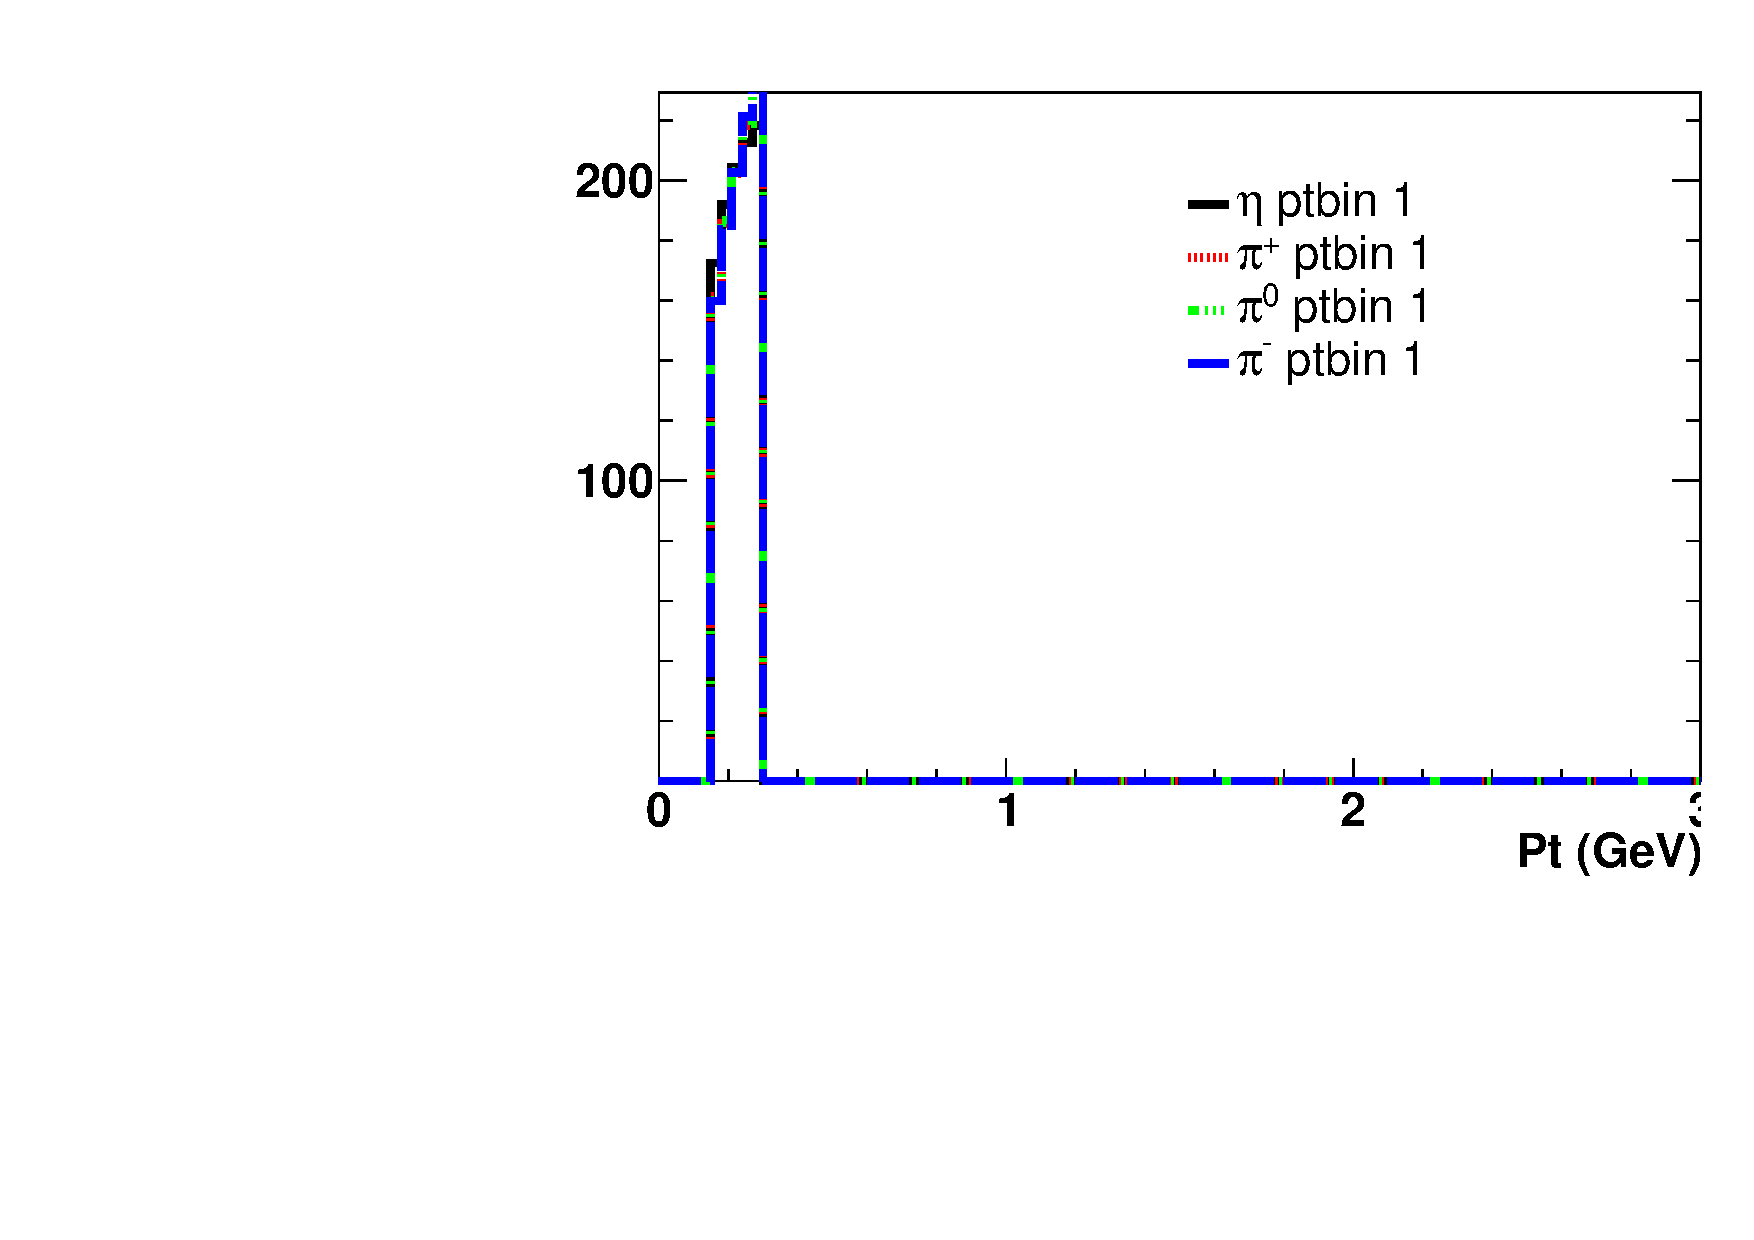
\includegraphics[width=.31\textwidth,natwidth=250,natheight=100]{figure_fiducial/had0.4_z0.3/Pt_distri_for_ptbin_1_norm_had04z03.pdf}\label{fig:kine_distri62}}
\caption{Normalized $P_t$ distributions of $\eta$ and pions for 0.15~GeV $<P_t<0.3$~GeV.}
\label{fig:kine_distri6}
\end{figure}

\begin{figure}[H]
\captionsetup[subfloat]{farskip=2pt,captionskip=1pt}
\centering
\subfigure[$H_{OA}<0.3$]{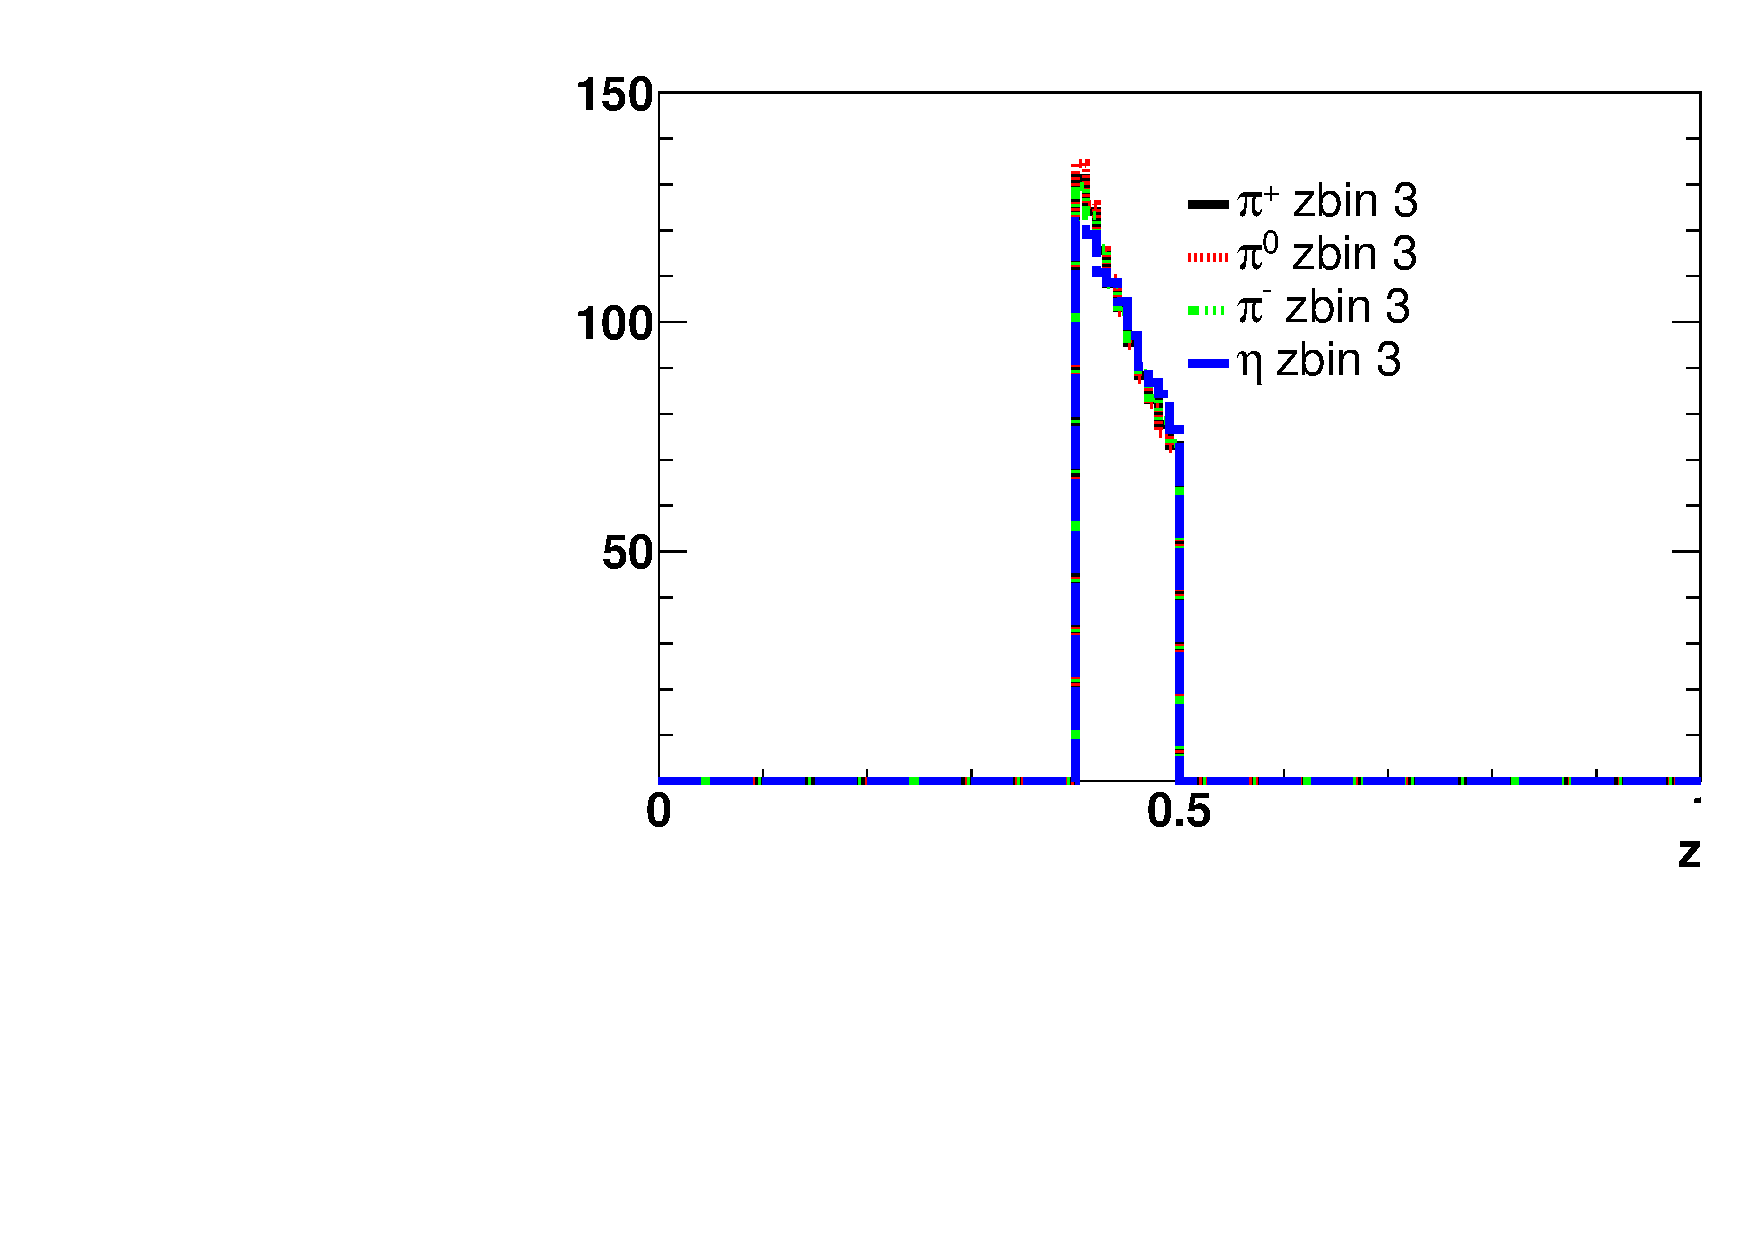
\includegraphics[width=.31\textwidth,natwidth=250,natheight=100]{figure_fiducial/had0.3_z0.3/Z_distri_for_zbin_3_norm_had03z03.pdf}\label{fig:kine_distri71}}
\subfigure[$H_{OA}<0.4$]{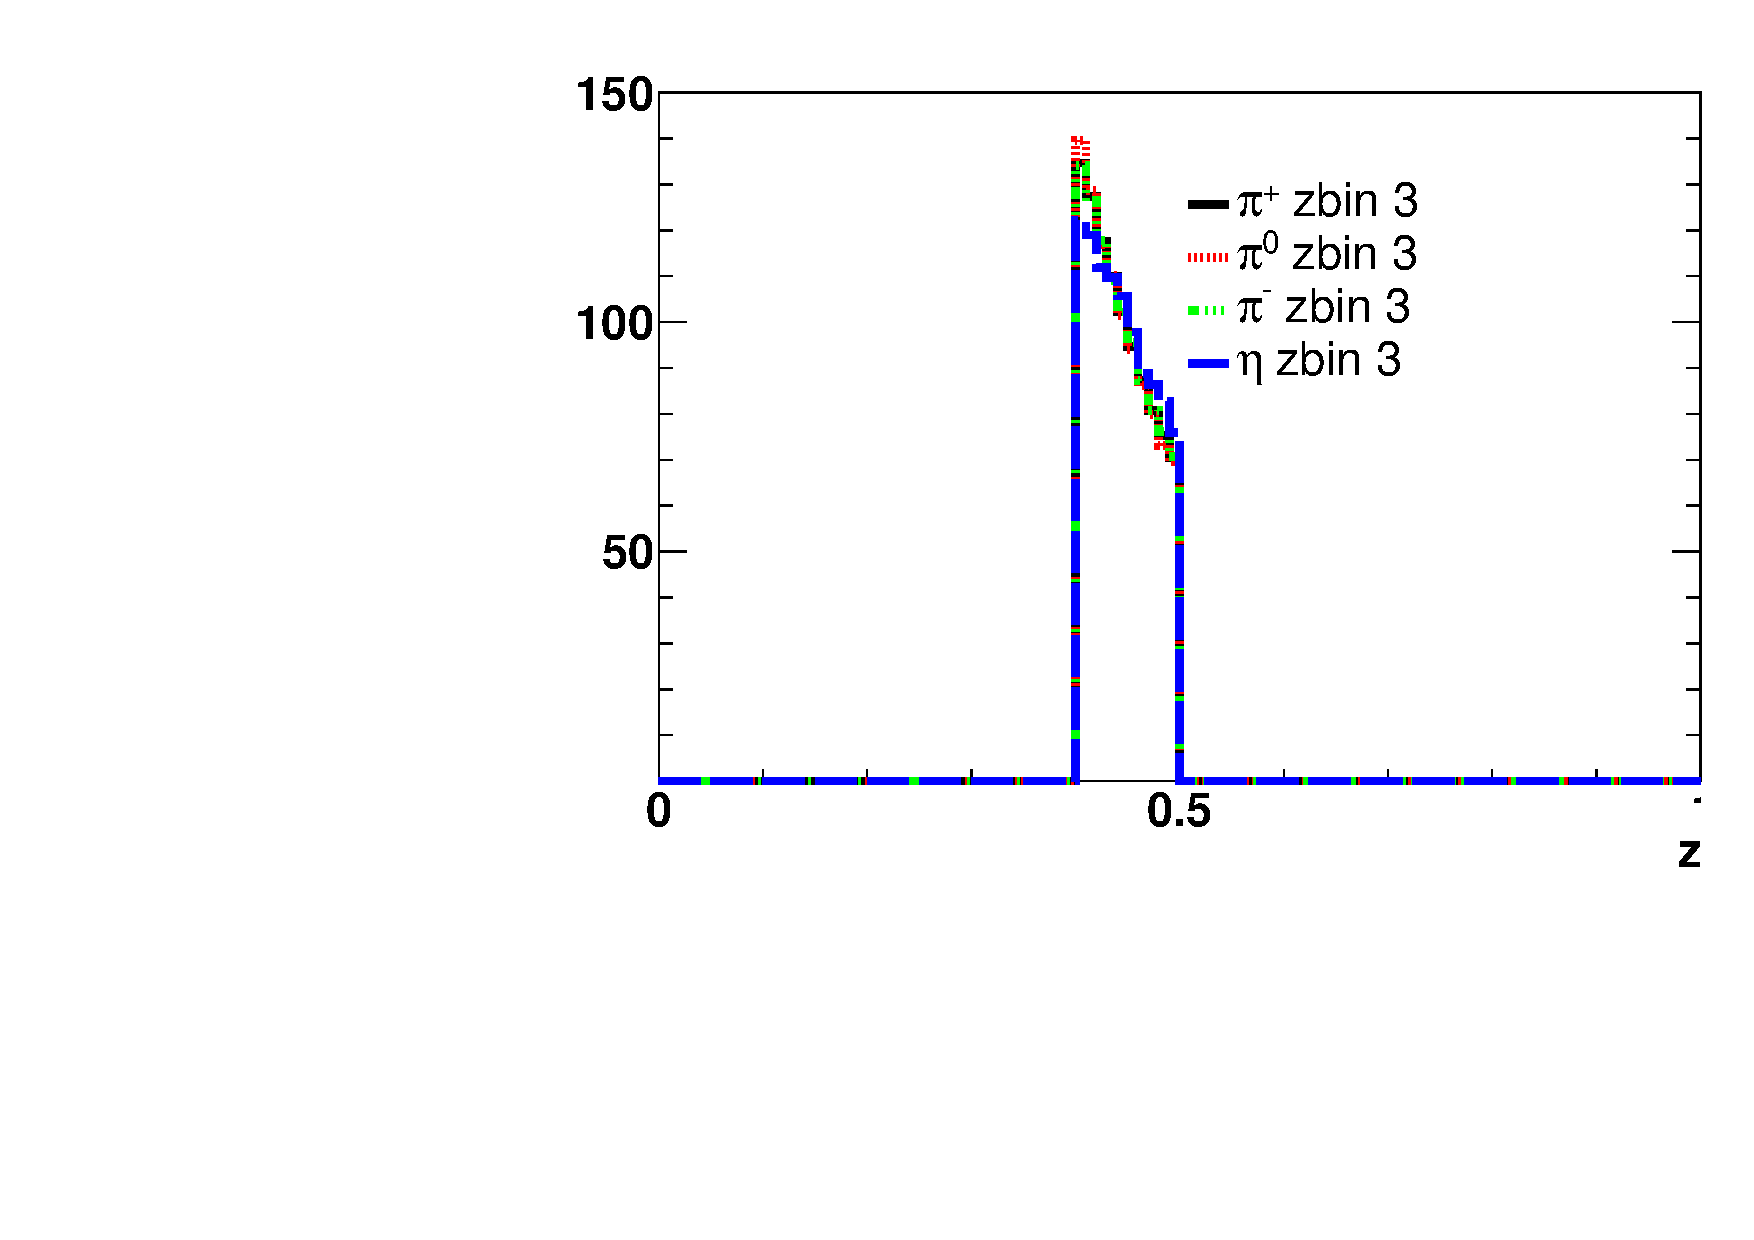
\includegraphics[width=.31\textwidth,natwidth=250,natheight=100]{figure_fiducial/had0.4_z0.3/Z_distri_for_zbin_3_norm_had04z03.pdf}\label{fig:kine_distri72}}
\caption{Normalized $z$ distributions of $\eta$ and pions for $0.4<z<0.5$.}
\label{fig:kine_distri7}
\end{figure}

\begin{figure}[H]
\captionsetup[subfloat]{farskip=2pt,captionskip=1pt}
\centering
\subfigure[$H_{OA}<0.3$]{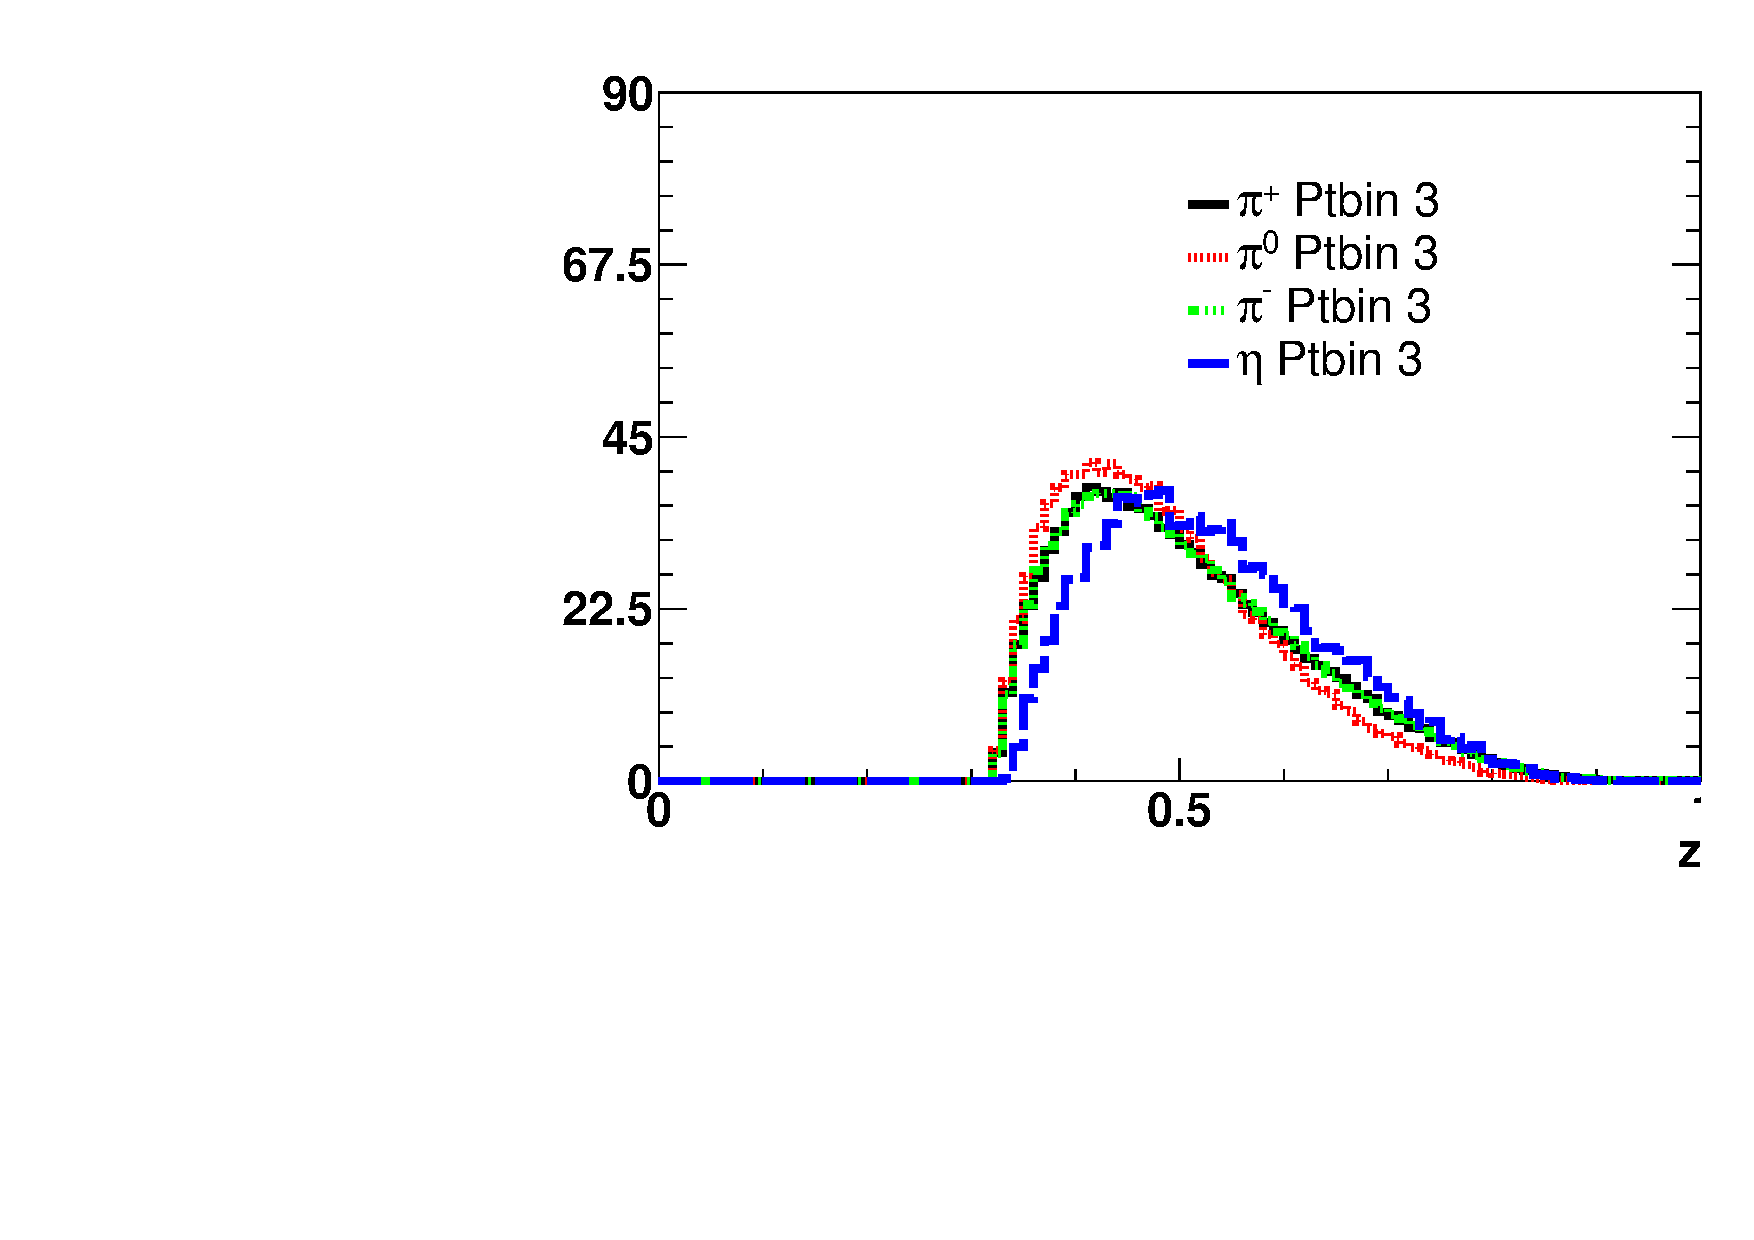
\includegraphics[width=.31\textwidth,natwidth=250,natheight=100]{figure_fiducial/had0.3_z0.3/Z_distri_for_ptbin_3_norm_had03z03.pdf}\label{fig:kine_distri81}}
\subfigure[$H_{OA}<0.4$]{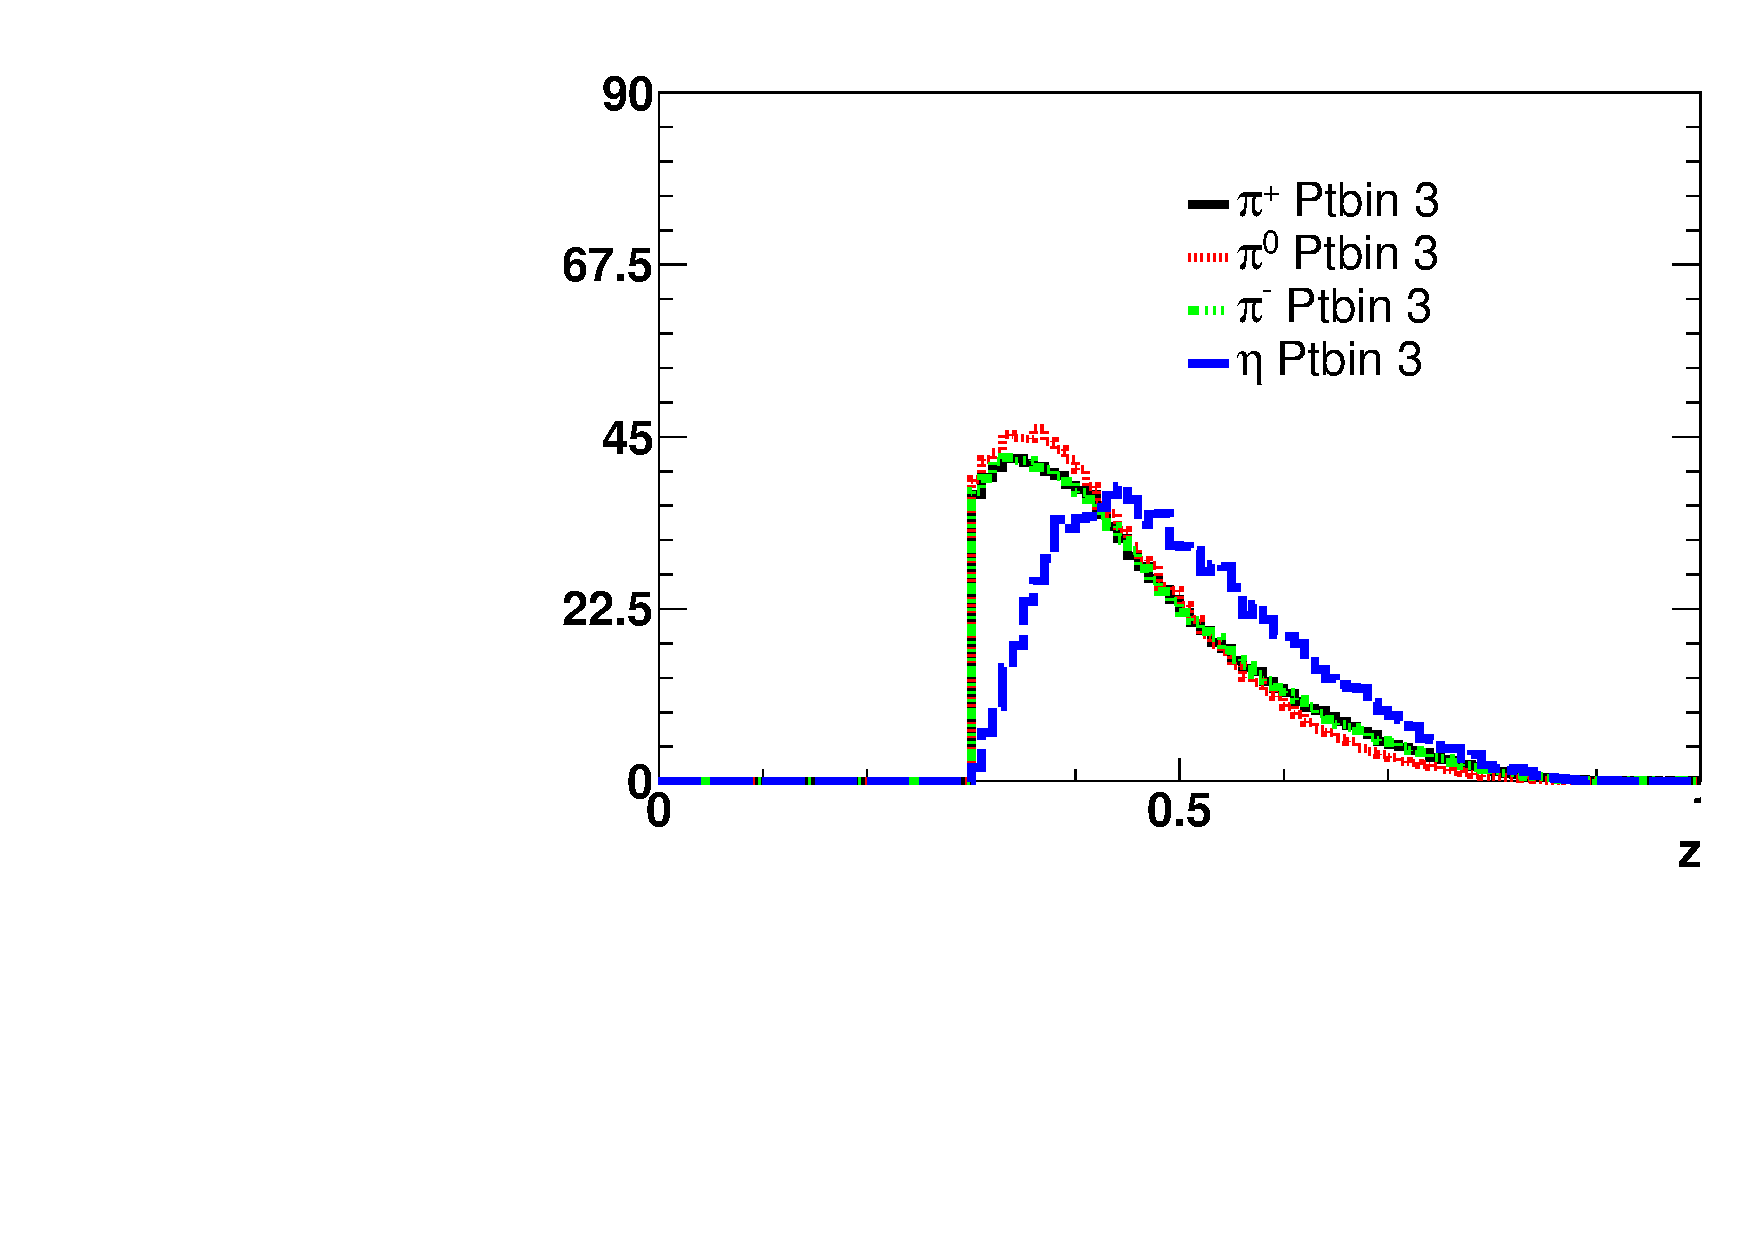
\includegraphics[width=.31\textwidth,natwidth=250,natheight=100]{figure_fiducial/had0.4_z0.3/Z_distri_for_ptbin_3_norm_had04z03.pdf}\label{fig:kine_distri82}}
\caption{Normalized $z$ distributions of $\eta$ and pions for 0.5~GeV $<P_t<3$~GeV.}
\label{fig:kine_distri8}
\end{figure}

By visually inspecting the distributions, we choose the maximum value of hadron to thrust opening angle ($H_{OA}$) as $0.3$ to get matching hadron-kinematics distributions. 



In summary, the principle behind the fiducial constraints summarized in Table~\ref{tab:constrain} is that all particles are captured by the barrel EMCAL, the hadrons are accepted symmetrically around the thrust axis and the acceptance for all hadrons is similar, indicated by similar kinematic distributions. With $\gamma_{OA}<0.5$ we obtain the highest FOM. Accordingly, $H_{OA}$ is set to 0.3 for all, i.e., charged and neutral, hadrons considered here to satisfy the requirement of similar geometric acceptance. Figure~\ref{fig:differentthetarange} compares the $\phi_1+\phi_2$ distribution for $\pi^0\pi^++\pi^0\pi^-$ pairs with and without applying the set of fiducial constraints. It can be seen that after applying the fiducial constraints, the amplitude of $R_{12}$ reduces significantly. This result also illustrates that  most of the false asymmetry comes from  detector effects since it can be removed by applying appropriate fiducial cuts. Last but not least, it should be noted that all these studies were performed on the Belle MC sample using PYTHIA6.1. The simulation does not contain the Collins effect, thus any remaining Collins-like cosine distribution originates from false asymmetries arising from detector-acceptance or gluon-radiation effects. 
\begin{figure}[h]
    \centering
    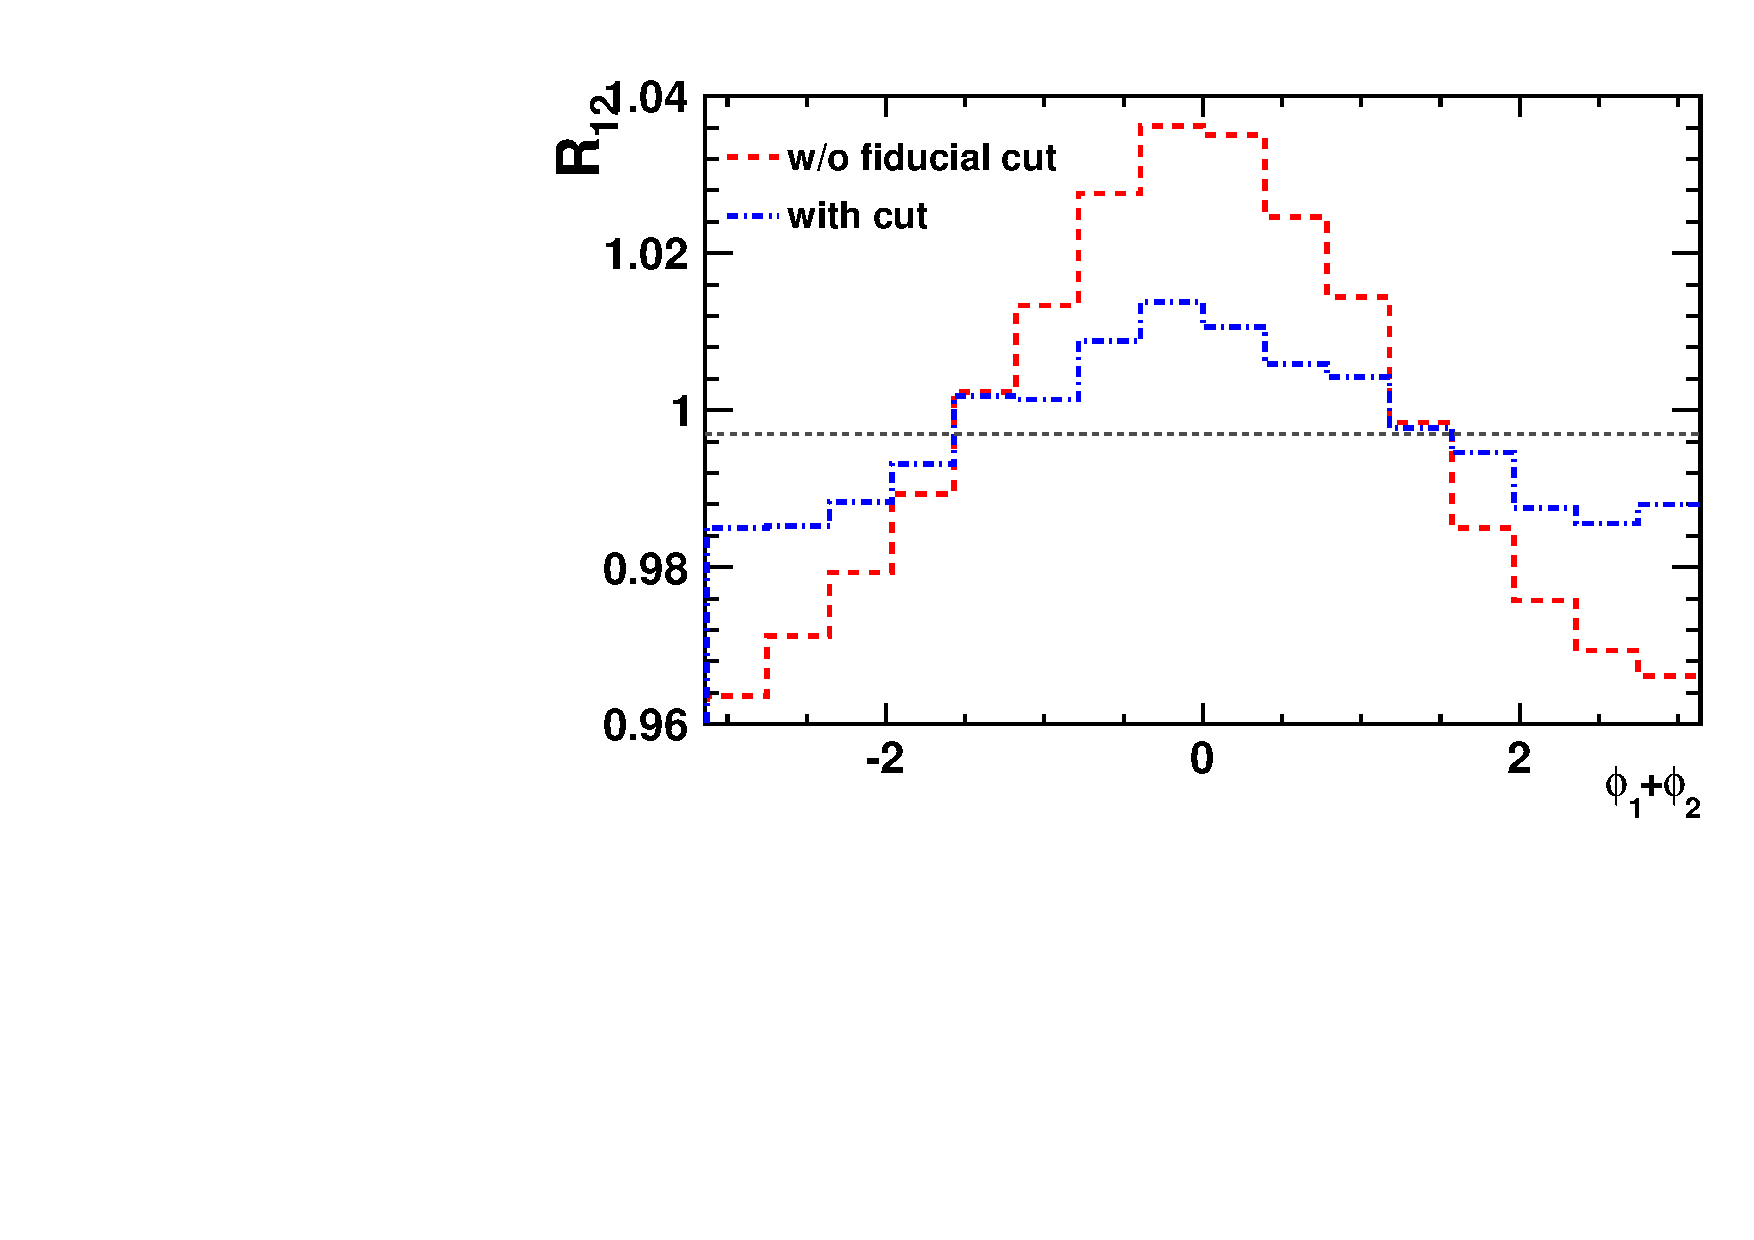
\includegraphics[width=0.55\textwidth,natwidth=610,natheight=642]{figure_dataselection/DetectorEffect.pdf}
    \caption[Normalized ratio $R_{12}$ for $\pi^0\pi^++\pi^0\pi^-$ with $0.3<z<0.4$ using MC data]{The normalized ratio $R_{12}$ for $\pi^0\pi^++\pi^0\pi^-$ with $0.3<z<0.4$ using MC data. The red histogram stands for the situation that no thrust or hadron direction cuts are applied. The blue histogram uses the criteria $\gamma_{OA} <0.3~\text{rad}$, $H_{OA}<0.5~\text{rad}$ and $1.34~\text{rad}<\theta<2.03~\text{rad}$.}
    \label{fig:differentthetarange}
\end{figure}


The final cuts on opening angle and photon energy are shown in Table~\ref{tab:constrain}. Note that the photon energy asymmetry cut is not listed since we determined that releasing this constraint optimizes the FOM.
%\begin{itemize}
%\item $\gamma$ energy constraint $50$~MeV for $\pi^0$, $150$~MeV for $\eta$.
%\item $z>0.1$ for hadrons forming double ratios that contain $\pi^0$.\footnote{For the kinematic bins where $z$ is  integrated, the threshold is increased to $z>0.2$. More details can be found in section~\ref{sec:kinematicbins}.}
%\item $z>0.3$ for hadrons forming double ratios that contain $\eta$, accounting for the higher $\eta$ mass and photon energy cut. 
%\end{itemize}

\begin{table}[H]\small
\centering
\begin{tabular}{|l|l|l|l|l|l|l|l|l|}
\hline
kinematic variable & constraint   \\ \hline
$E_\gamma$~($\pi^0$) & $E_\gamma >50$~MeV \\ \hline
$E_\gamma$~($\eta$) & $E_\gamma >250$~MeV \\ \hline
$z$  for hadrons forming double ratios &\multirow{2}{*}{$z>0.1$}\\
 that contain $\pi^0$&  \\ \hline
$z$ for hadrons forming double ratios that contain $\eta$,& \multirow{3}{*}{$z>0.3$} \\ accounting for the higher $\eta$ mass &\\and photon energy cut & \\ \hline
$\gamma_{OA}$ (modulo $\pi$) & $<0.5$~rad \\ \hline
$H_{OA}$ (modulo $\pi$) & $<0.3$~rad \\ \hline
$\theta$ &  1.34~rad  --  2.03~rad  \\ \hline
\end{tabular}
\caption{Fiducial and energy constraints for $\pi^0$ and $\eta$.
For the kinematic bins of $\pi^0$ asymmetries where $z$ is  integrated, the threshold is increased to $z>0.2$. More details can be found in section~\ref{sec:kinematicbins}.
}
\label{tab:constrain}
\end{table}

\subsection{Neutral-Meson Reconstruction}
\label{sec:neutralmesonreconstruction}

This section discusses the reconstruction of the neutral mesons. In particular, we discuss different fitting techniques to the two photon invariant mass spectrum to extract the $\pi^0$ yield in Sections~\ref{sec:pi0fitsection}-\ref{sec:fit_with_MC_BG} and the fits to extract the $\eta$ yield in Section~\ref{sec:etafitsection}. Finally, we optimize the mass windows for the neutral-meson extractions in Section~\ref{sec:masswindow}. The input to the fits described in this section are photon pairs that fulfill the energy constraints outlined in the previous Section~\ref{sec:fidAndEnergyCuts}. 
These cuts suppress background from detector noise as well as combinatorial background.

\subsubsection{\texorpdfstring{Invariant-Mass Fit of $\pi^0$}{pi0 fit}}
\label{sec:pi0fitsection}
A reasonably good fit to the $\pi^0$ invariant-mass spectrum can be achieved by using a polynomial function for the background and a Gaussian for the signal. However, we observed that the signal has large tails below the nominal $m_{\pi^0}$. From simulation we could determine the reason: If a photon splits via  $\gamma\rightarrow e^+e^-$, one of the leptons can be lost, while the other is initiating an electromagnetic shower in the EMCAL and gets mistaken for a photon.
 Therefore, we decided to use the Crystal Ball function to fit the signal, since it can accommodate the observed asymmetric tails.  This fit is described in Section~\ref{sec:crystalBallFit}.
 It is also possible to extract the $\pi^0$ yield via a nonparametric method. For this we estimate the background shape from the simulation in the sidebands, extrapolate into the signal region, and subtract the background to extract the signal.  This fitting method is described in Section~\ref{sec:fit_with_MC_BG}.
For the final results we use the Crystal-Ball fit and take the difference of those two fitting methods as a contribution to the systematic uncertainty.

\subsubsection{Fit with the Crystal-Ball Function}
\label{sec:crystalBallFit}
We use a polynomial function of degree 5 and Crystal Ball function to describe the background and signal. The Crystal Ball function of $x$ is defined as~\cite{CrystalBallFunc}
\begin{subequations}
\begin{align}
f(x;\alpha,n,\bar x,\sigma) & = N \cdot \begin{cases} \exp(- \frac{(x - \bar x)^2}{2 \sigma^2}), & \mbox{for }\frac{x - \bar x}{\sigma} > -\alpha \\
 A \cdot (B - \frac{x - \bar x}{\sigma})^{-n}, & \mbox{for }\frac{x - \bar x}{\sigma} \leqslant -\alpha \end{cases}\\
A & = \left(\frac{n}{\left| \alpha \right|}\right)^n \cdot \exp\left(- \frac {\left| \alpha \right|^2}{2}\right), \\
B &= \frac{n}{\left| \alpha \right|}  - \left| \alpha \right|,\\
%N &=\frac{1}{\sigma(C+D)},
%C &=\frac{n}{\left|\alpha \right| \cdot \frac{1}{n-1} \cdot \exp(-\frac{\left| \alpha \right|^2}{2}),\\
%D &=\sqrt{\frac{\pi}{2}}(1+\DeclareMathOperator\erf{erf}(\frac{\left| \alpha \right|}{\sqrt{2}}))
N &= \frac{1}{\sigma (C + D)}\\
C &= \frac{n}{\left| \alpha \right|} \cdot \frac{1}{n-1} \cdot \exp\left(- \frac {\left| \alpha \right|^2}{2}\right) \\
D &= \sqrt{\frac{\pi}{2}} \left(1 + \operatorname{erf}\left(\frac{\left| \alpha \right|}{\sqrt 2}\right)\right) 
\end{align}
\label{eqn:crystalball}
\end{subequations}
%Here the parameters $\sigma$ and $\bar x$ control the shape of the function similarly to the width and mean of a Gaussian. 

Figure~\ref{fig:pi0_crystalfit} contains some fitting examples. More plots can be found in Appendix~\ref{sec:cryfitpi0}. 
%min=0.055,max=0.22 
The vertical black dash lines in the plots are boundaries of the signal mass window that we will discuss in Section~\ref{sec:masswindow}. 
The fitting result (blue line) shows good agreement with experimental data except for some slight differences in sideband regions. 

\begin{figure}
  \centering     
  \subfigure[$\pi^0$ invariant-mass fit, $P_t<0.15$~GeV]{\label{fig:pi0crystalfit_1}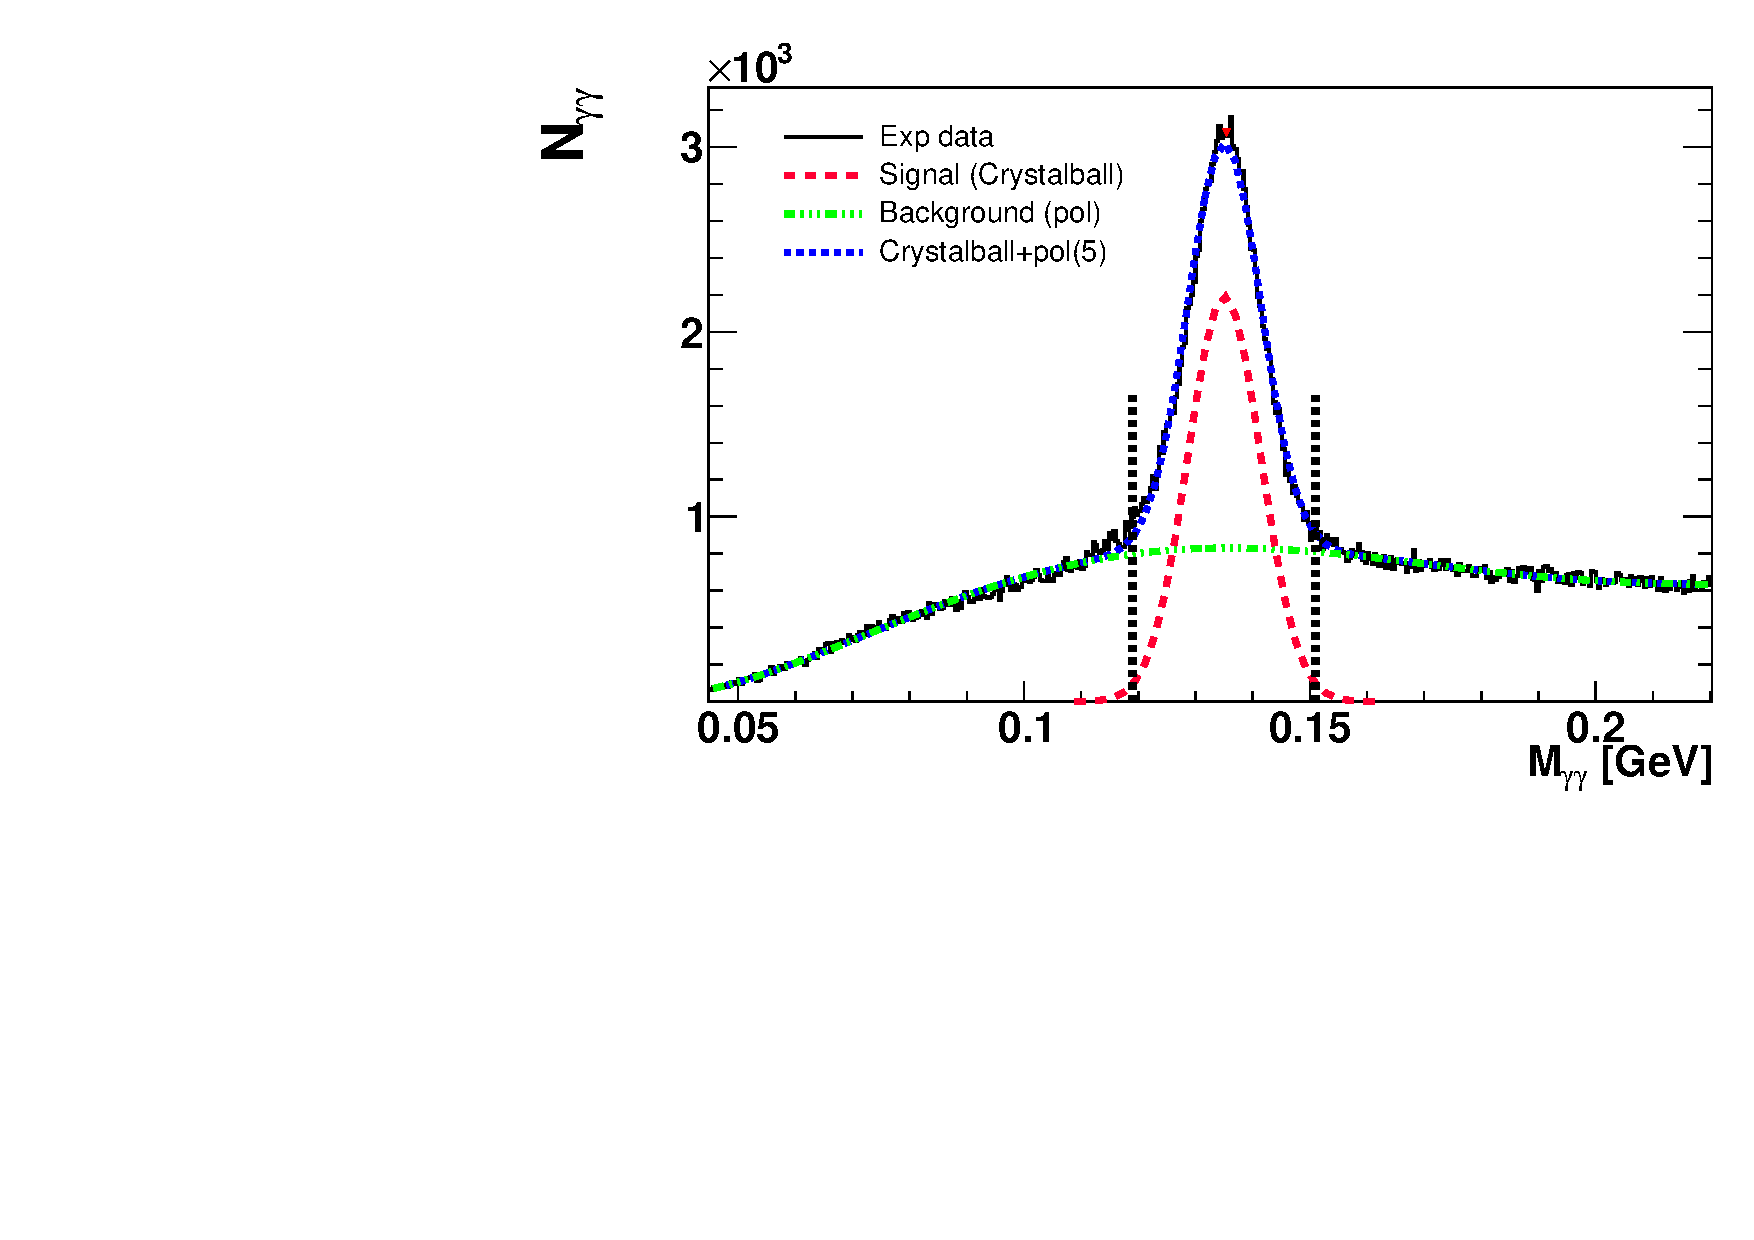
\includegraphics[width=.48\textwidth,natwidth=600,natheight=400]{figure_dataselection/pi0_crystalfit_Pt_0.pdf}}
  \subfigure[$\pi^0$ invariant-mass fit, 0.3~GeV $<P_t<0.5$~GeV]{\label{fig:pi0crystalfit_2}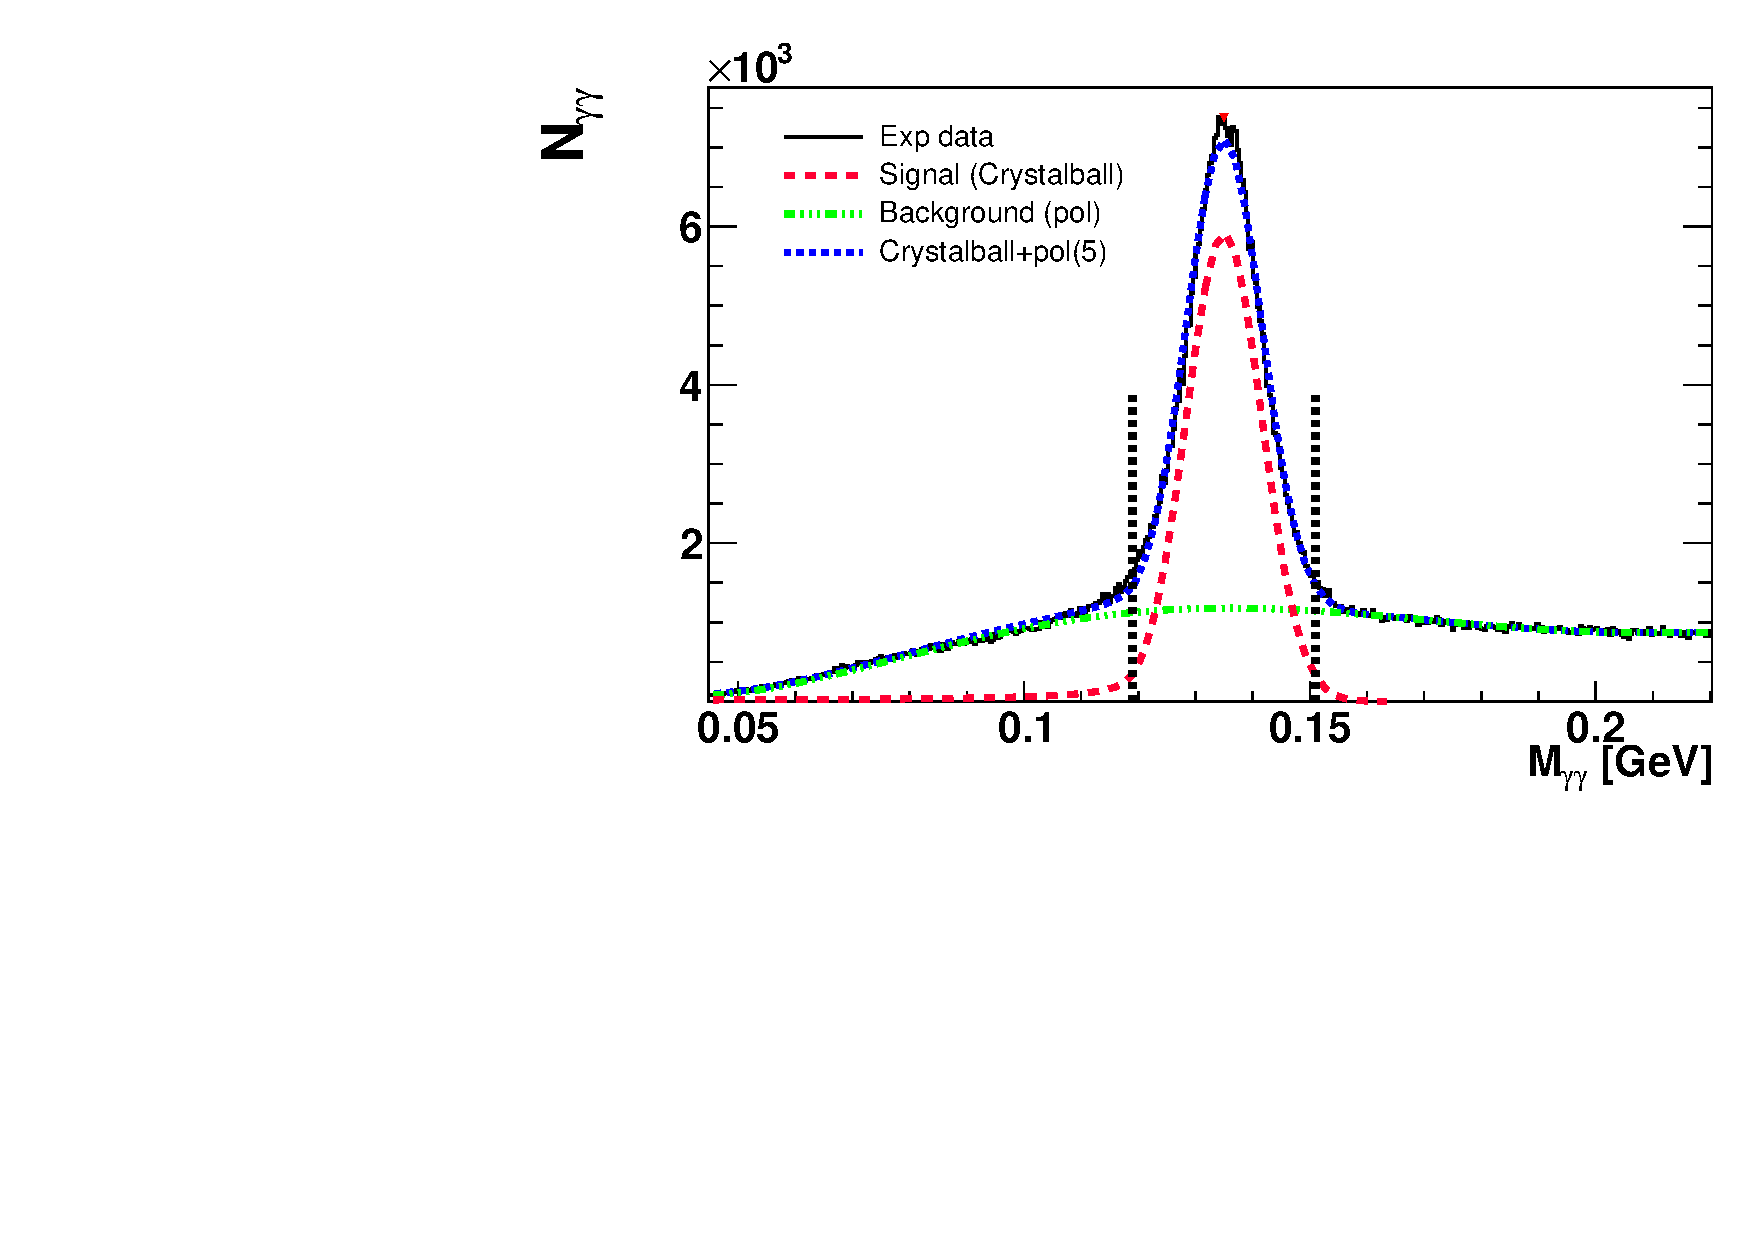
\includegraphics[width=.48\textwidth,natwidth=600,natheight=400]{figure_dataselection/pi0_crystalfit_Pt_2.pdf}}
  \subfigure[$\pi^0$ invariant-mass fit, $0.2<z<0.3$]{\label{fig:pi0crystalfit_3}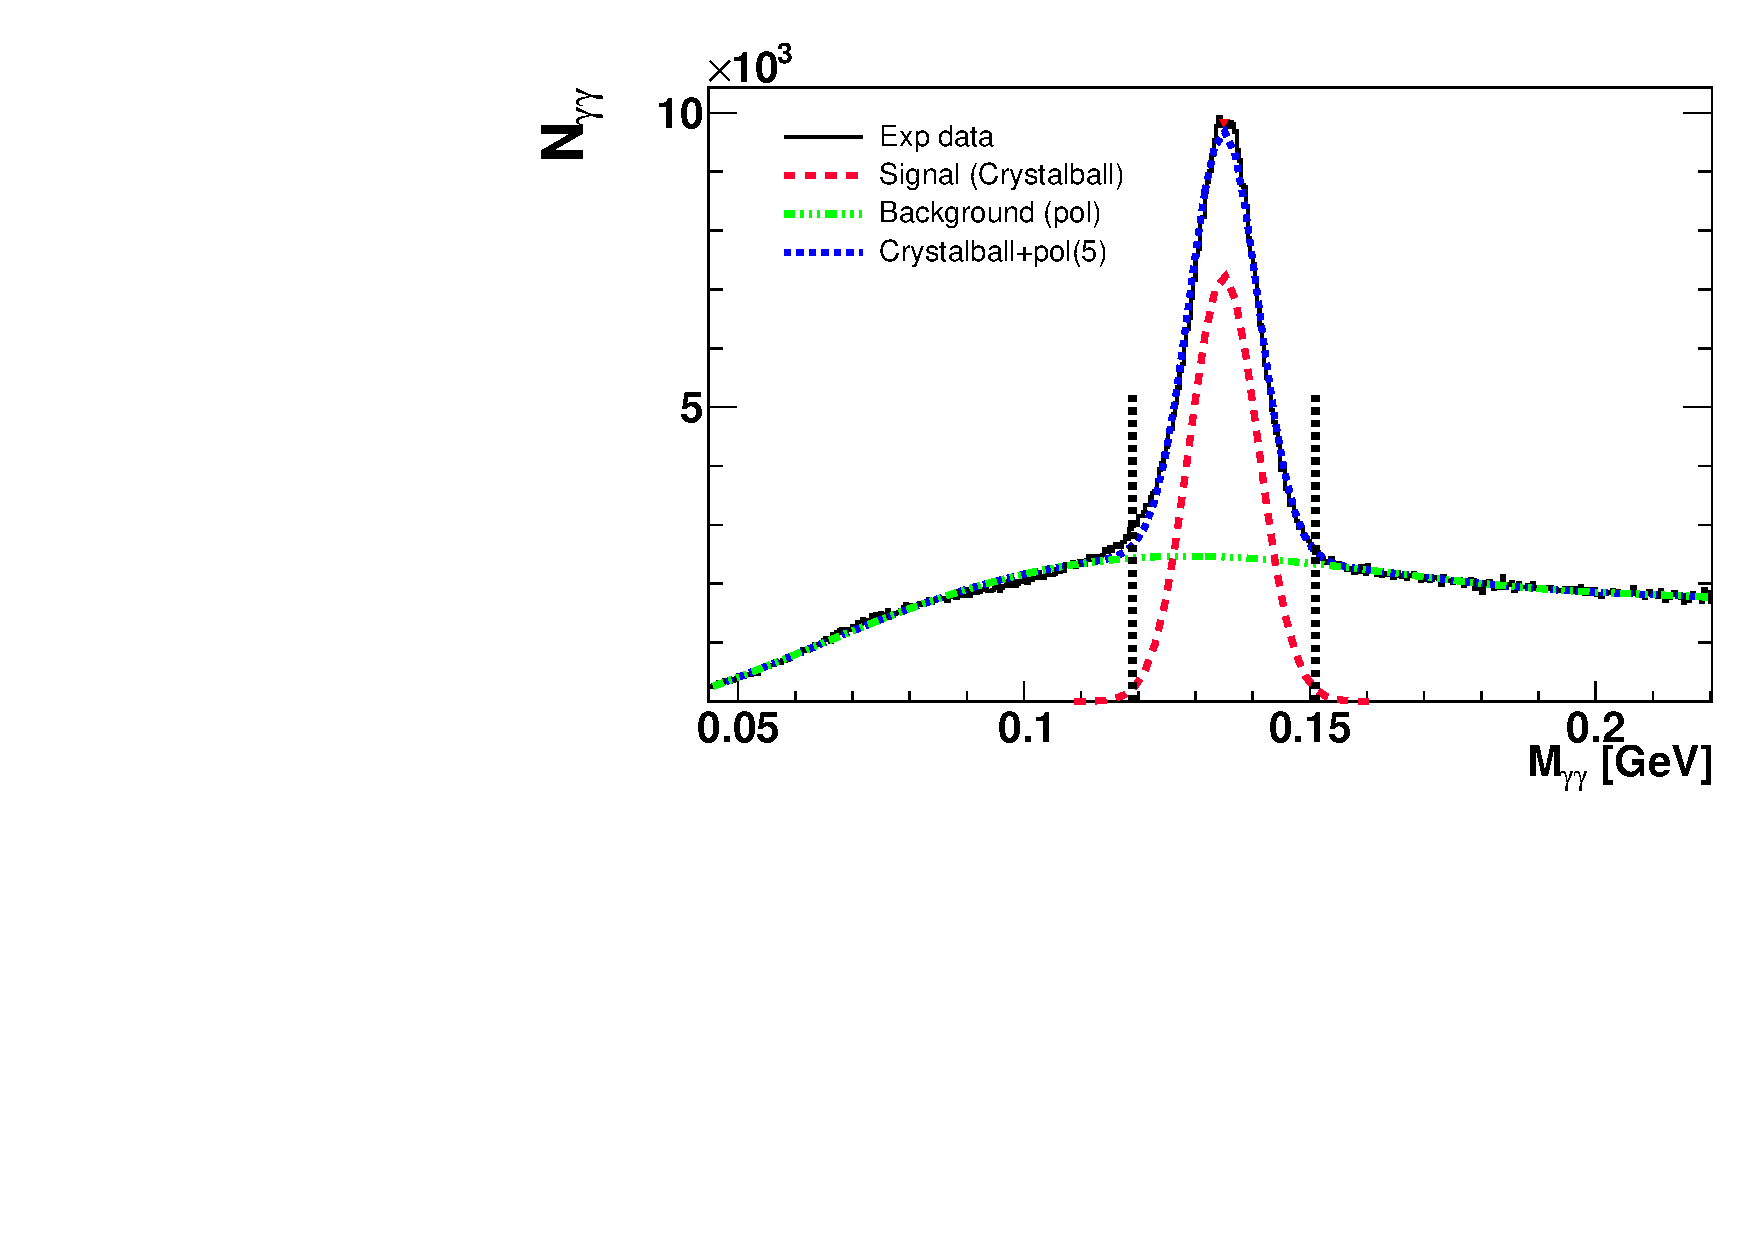
\includegraphics[width=.48\textwidth,natwidth=600,natheight=400]{figure_dataselection/pi0_crystalfit_Z_1.pdf}}
  \subfigure[$\pi^0$ invariant-mass fit, $0.6<z<0.7$]{\label{fig:pi0crystalfit_4}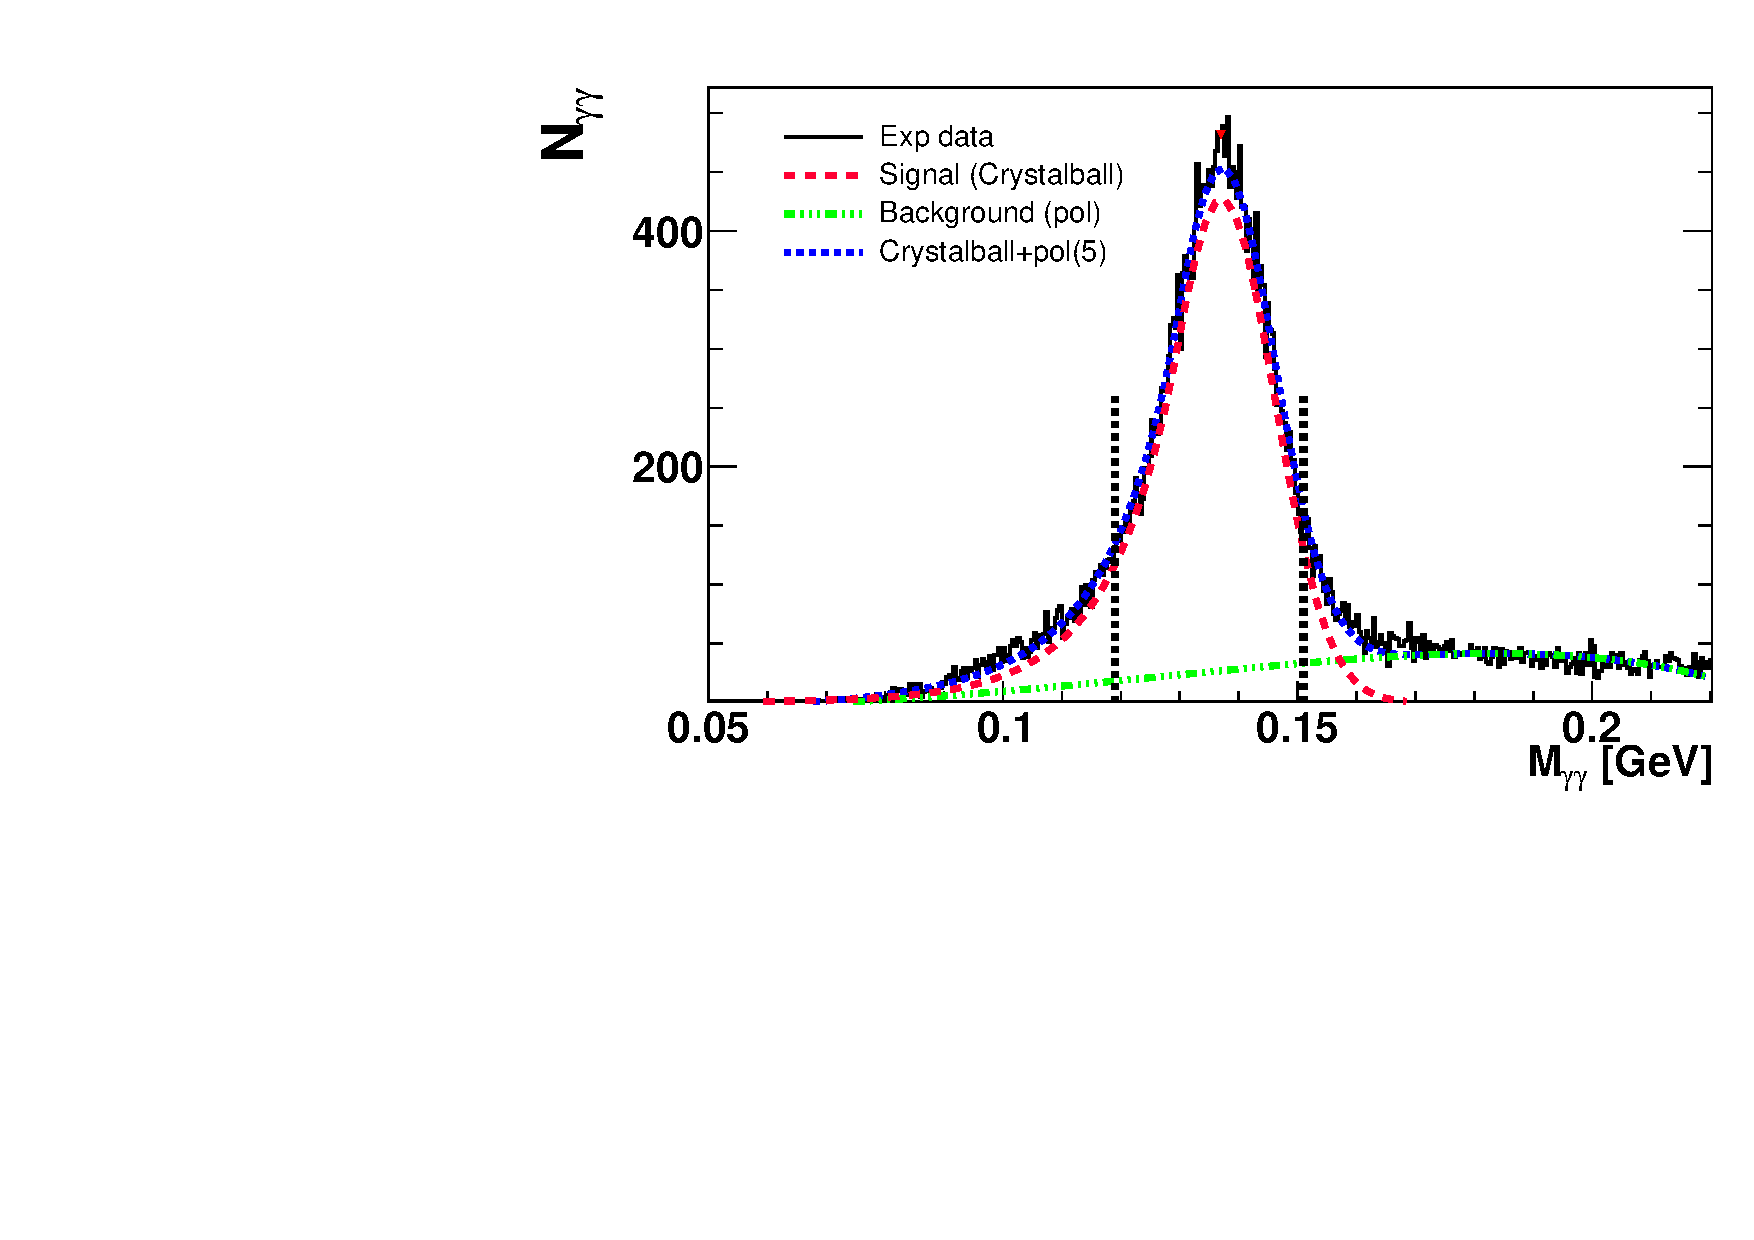
\includegraphics[width=.48\textwidth,natwidth=600,natheight=400]{figure_dataselection/pi0_crystalfit_Z_5.pdf}}
      \caption[Fit to the two-photon invariant-mass distribution using a Crystal Ball function for the signal and a polynomial background function]{Fit to the two-photon invariant mass distribution using a Crystal Ball function for the signal and a polynomial background function. In each plot, the green line represents the fitted background using a polynomial of 5th order, the red line the fitted signal and the blue line is the combined background and signal fit. It agrees well with the experimental data in black. The vertical dash lines are the boundaries that we will use to select the signal. See text for more details.}
  \label{fig:pi0_crystalfit}
\end{figure}

\subsubsection{Fit with Monte Carlo Background}
\label{sec:fit_with_MC_BG}

The fits presented in the previous section agree well with the experimental data. 
However, the question if we actually extract the correct background fraction is predicated on the condition that we get the signal and background shape correct.  One particular question is, how much the signal `bleeds' into the sideband region which has the most impact on the background fit. In this section we  develop an alternative, non-parametric method to extract the signal based on the shapes of signal and background as obtained from simulation. The advantage of this method is that it can differentiate between signal and background in regions where their shapes are similar. On the other hand, it relies of course on a correct description of the experimental data in the simulation.
%One of the main questions in the background evaluation is: Does 
%the event sample used for the BG obtained from the previous fits reflect 
%to a good degree the characteristics of the BG under the signal peak? 
%After all we want to separate the actual signal ("true" pi0) asymmetry 
%from the total asymmetry in this invariant-mass range by subtracting the 
%BG asymmetry. The latter has to be obtained from a different event sample 
%and if part of the sidebands is correlated with the signal asymmetry, 
%those sideband bins might not be a good proxy in the BG subtraction in particular since they can contain signal events where one of the decay $\gamma$ lost energy in pair creation (and one of the resulting leptons was misidentified as a $\gamma$). Hence 
%the studies presented in this section."
%Although the last section shows good fitting result, we still need to figure out if the components of the reconstruction are precisely described.
Some exemplary comparisons of the signal-background separated simulations with experimental data are shown in  Fig.~\ref{fig:pi0MC_Exp}. We observe that the agreement in the sidebands is quite good.  For low-$z$ and low-$P_t$ bins,  shown in Fig.~\ref{fig:pi0mcexp_1} and Fig.~\ref{fig:pi0mcexp_3} significant differences between Monte Carlo and experimental data can be seen in the signal region, seemingly caused by an overestimation of the signal yield in the MC. The agreement in the signal and background regions at high $P_t$ and high $z$ is quite good. 

\begin{figure}
  \centering     
  \subfigure[$\pi^0$ invariant mass, $P_t<0.15$~GeV]{\label{fig:pi0mcexp_1}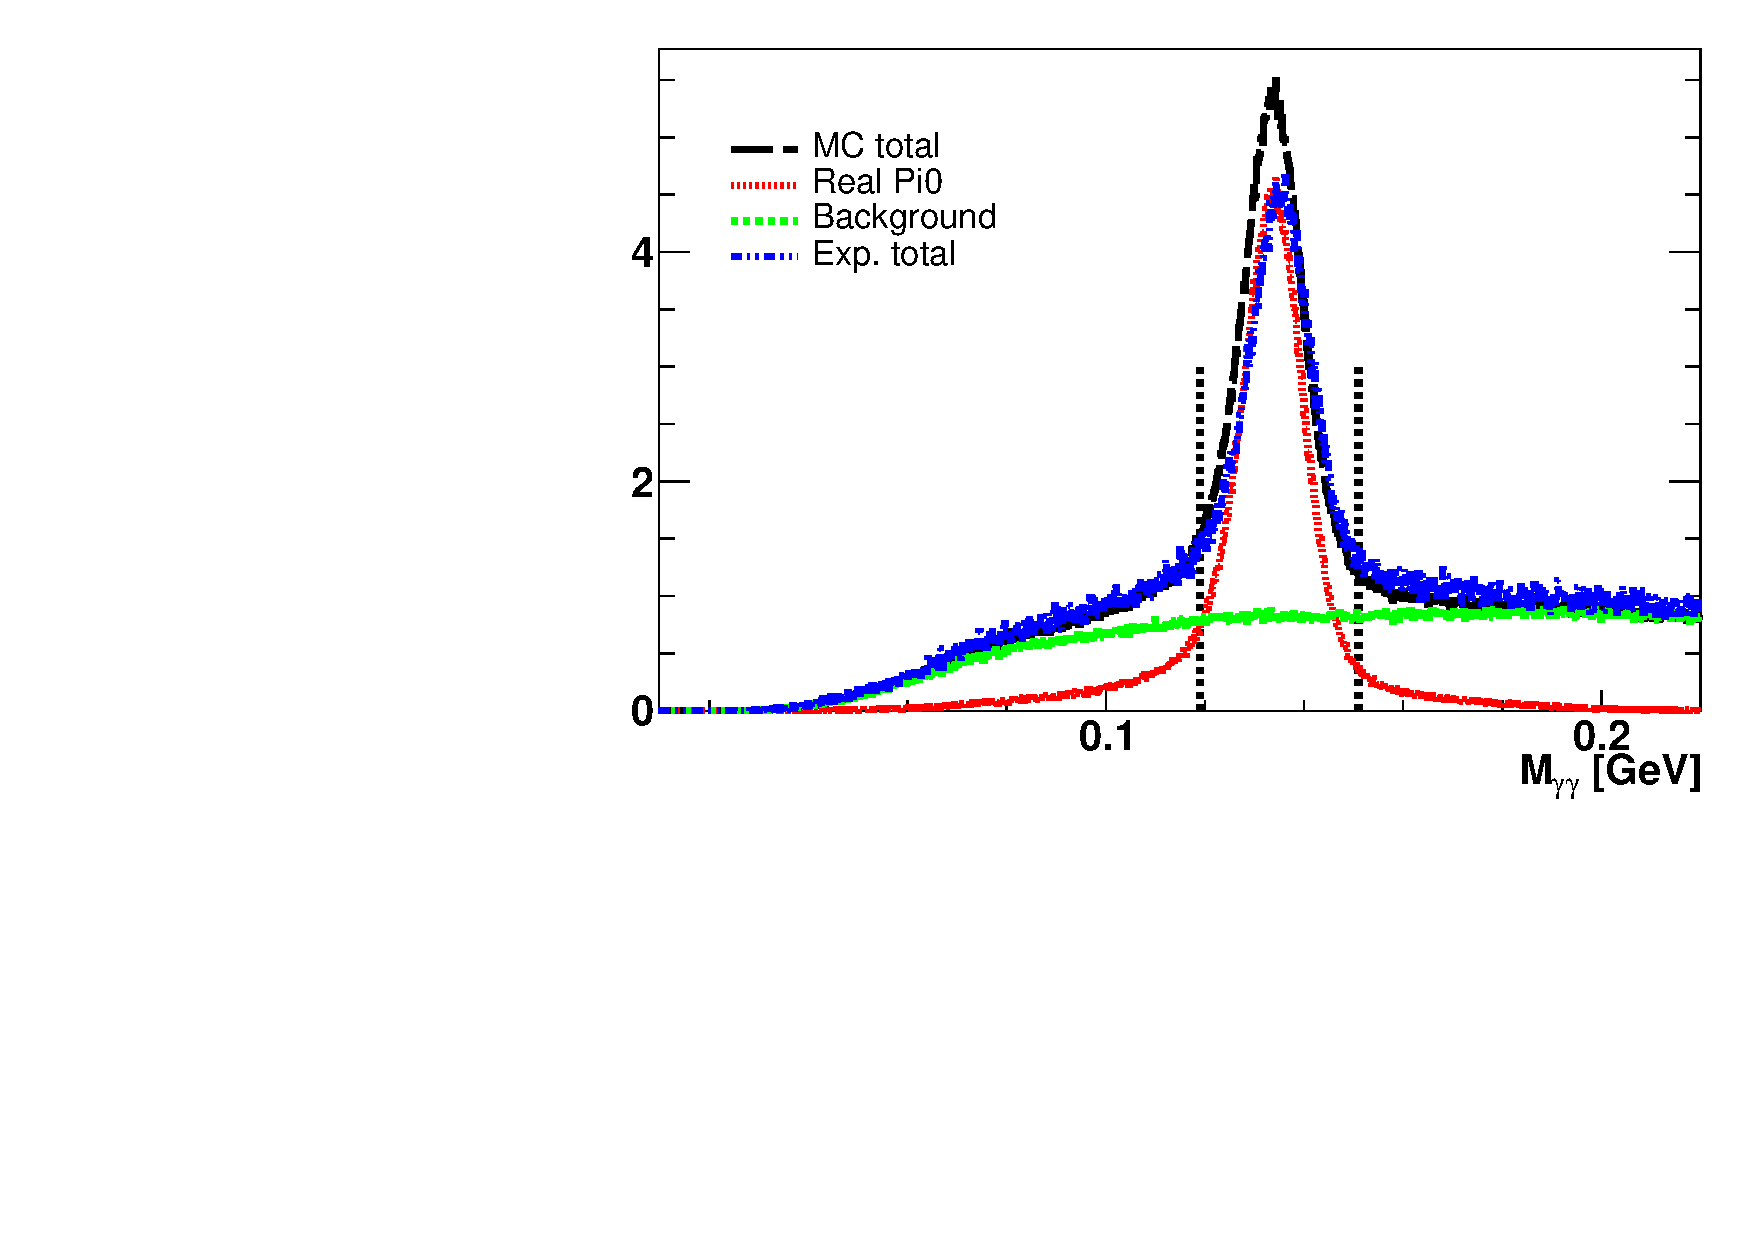
\includegraphics[width=.48\textwidth,natwidth=250,natheight=100]{figure_dataselection/pi0_Pt_0.pdf}}
  \subfigure[$\pi^0$ invariant mass, 0.3~GeV $<P_t<0.5$~GeV]{\label{fig:pi0mcexp_2}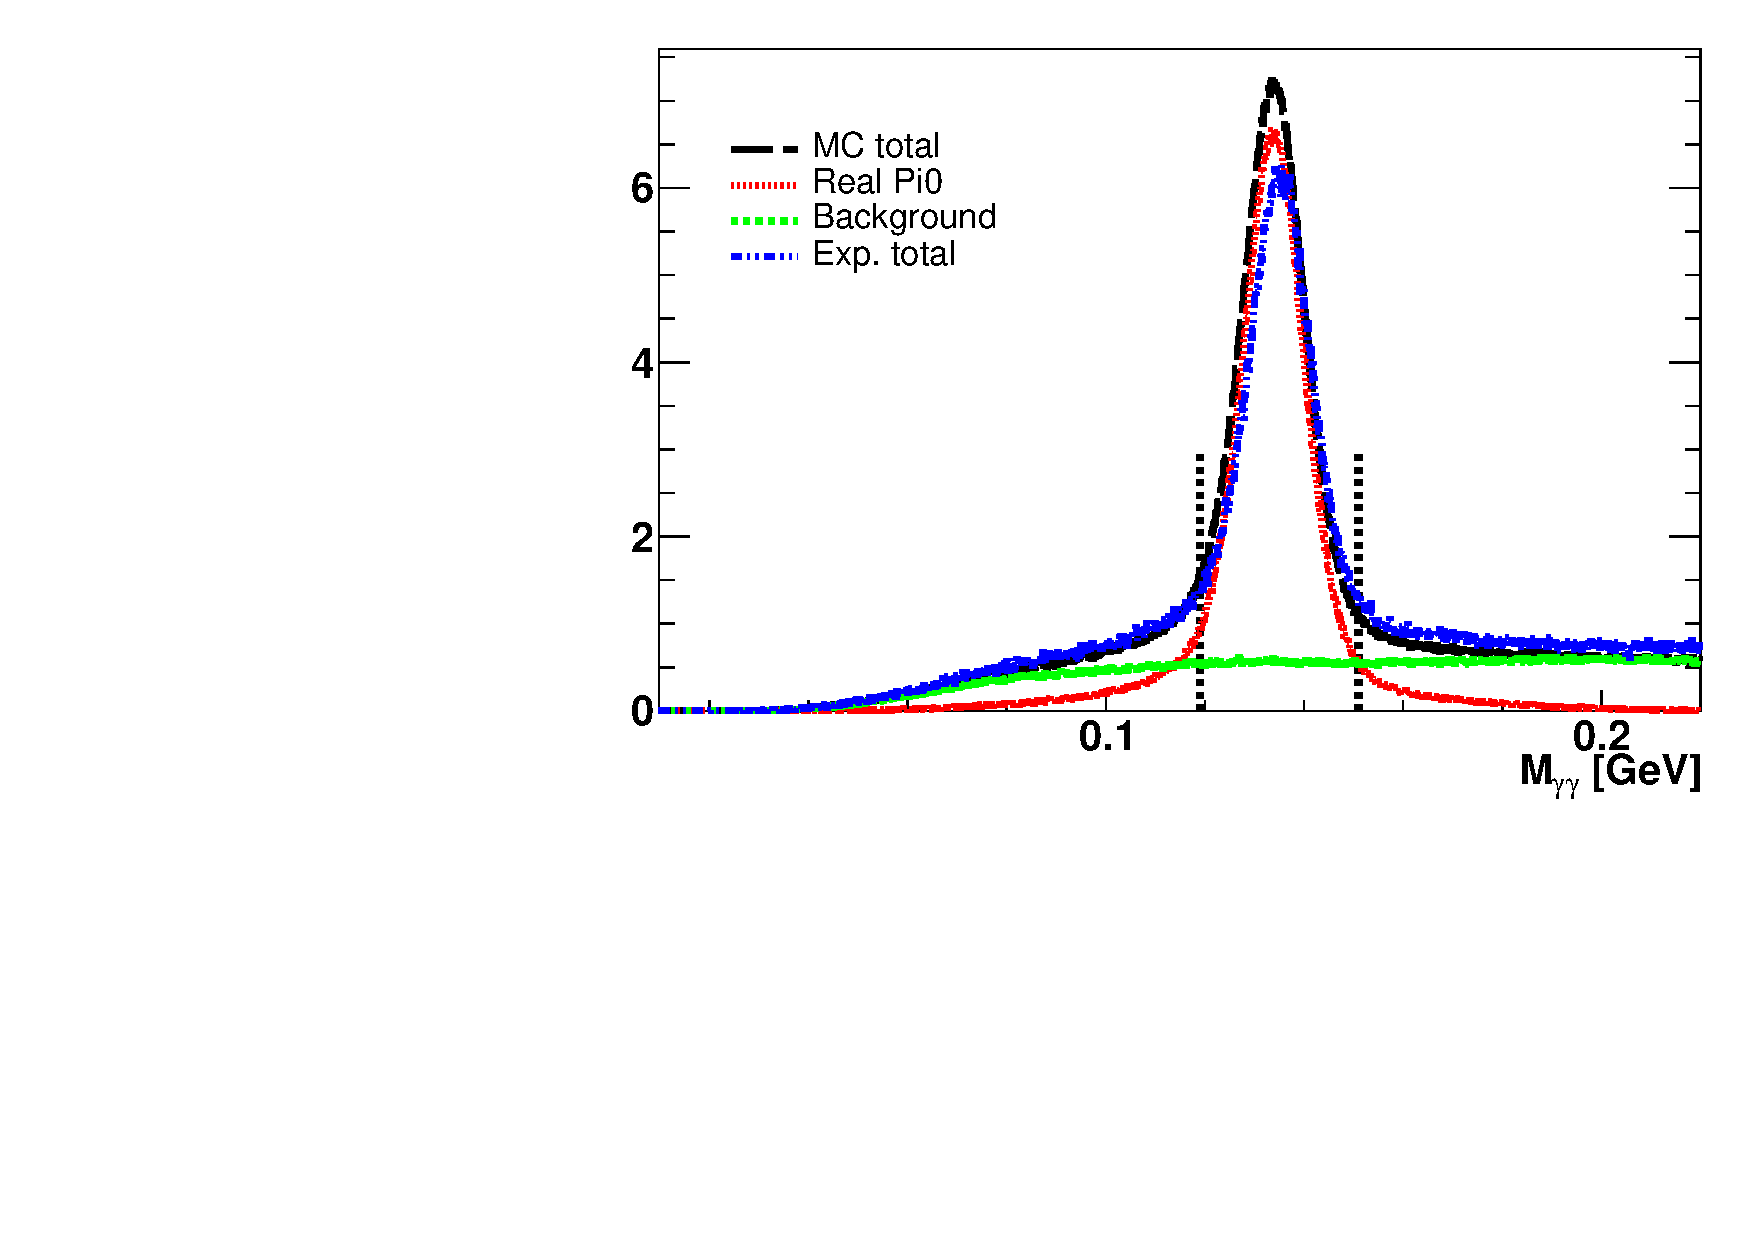
\includegraphics[width=.48\textwidth,natwidth=250,natheight=100]{figure_dataselection/pi0_Pt_2.pdf}}
   \subfigure[$\pi^0$ invariant mass, $0.2<z<0.3$]{\label{fig:pi0mcexp_3}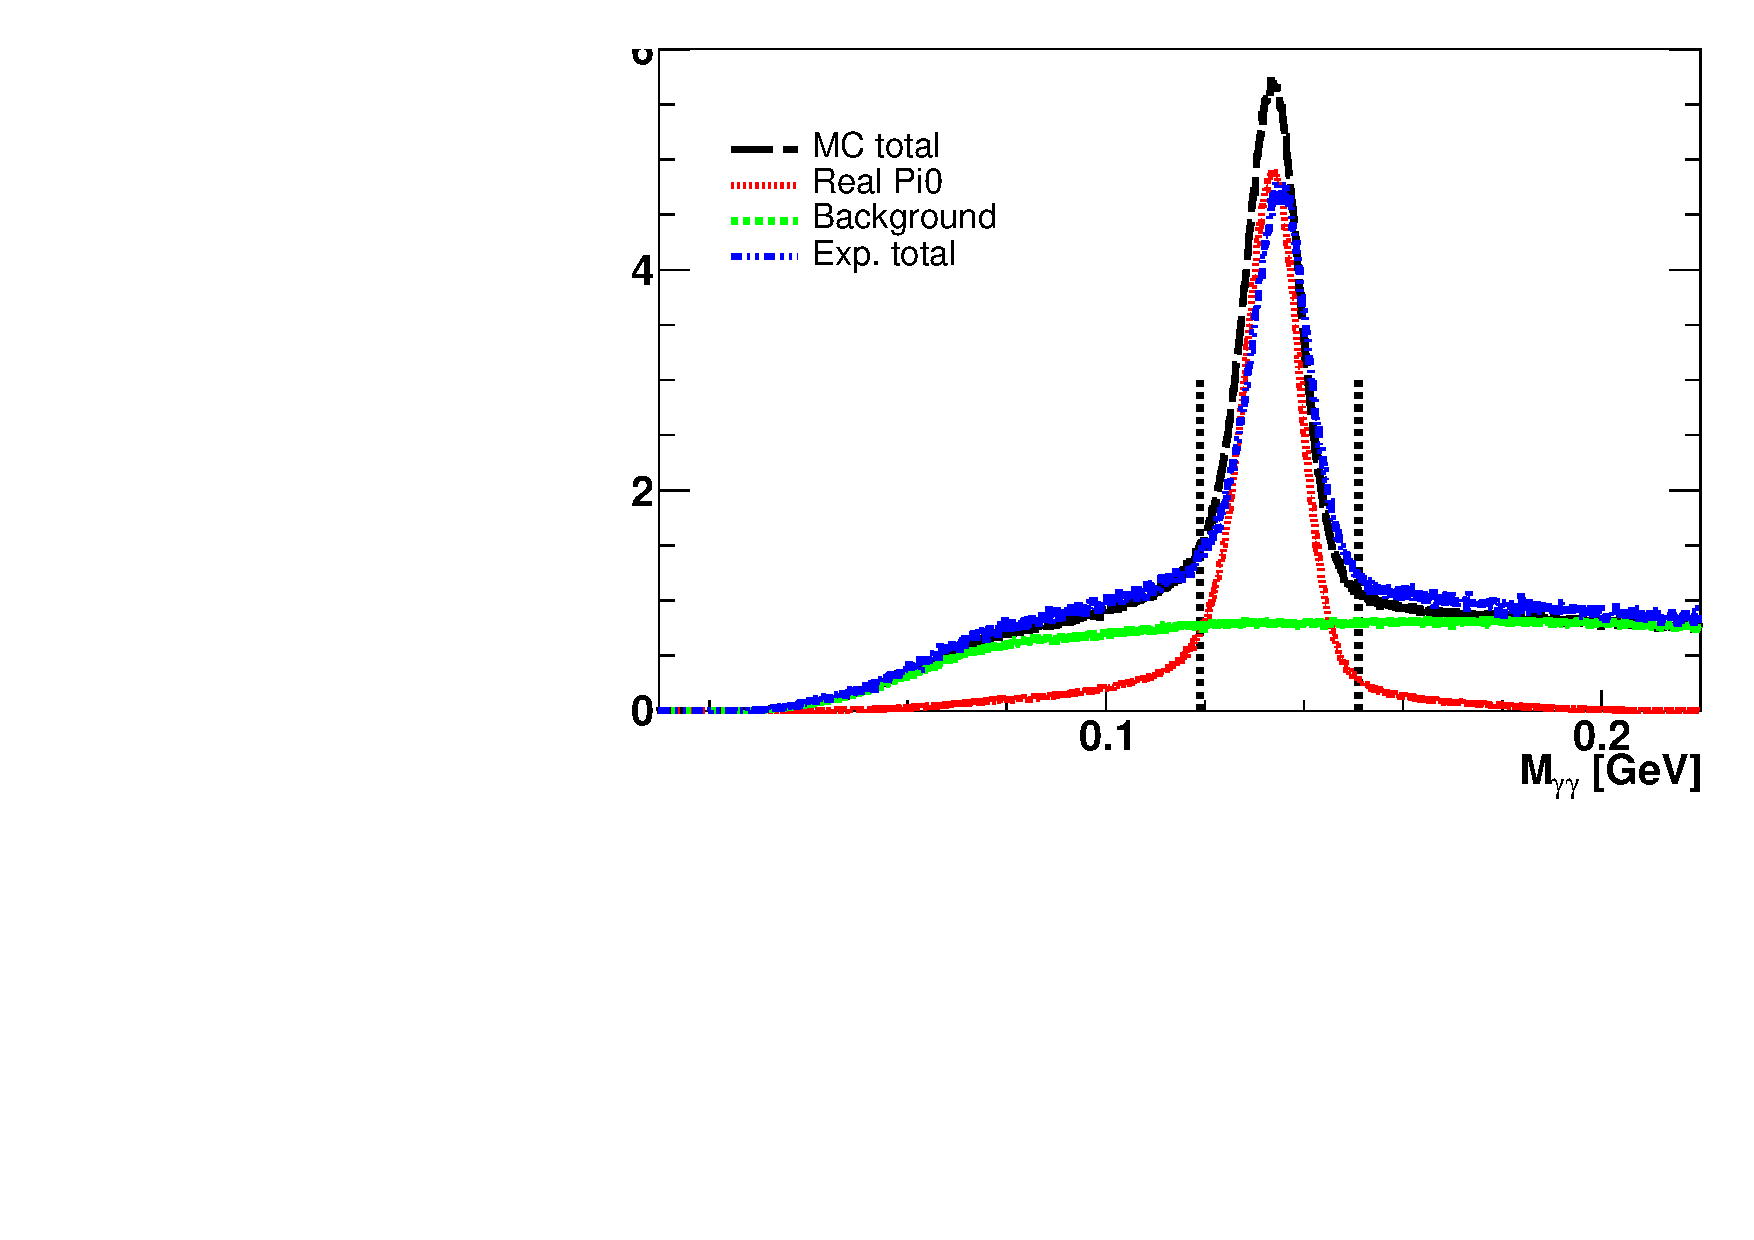
\includegraphics[width=.48\textwidth,natwidth=250,natheight=100]{figure_dataselection/pi0_Z_1.pdf}}
  \subfigure[$\pi^0$ invariant mass, $0.6<z<0.7$]{\label{fig:pi0mcexp_4}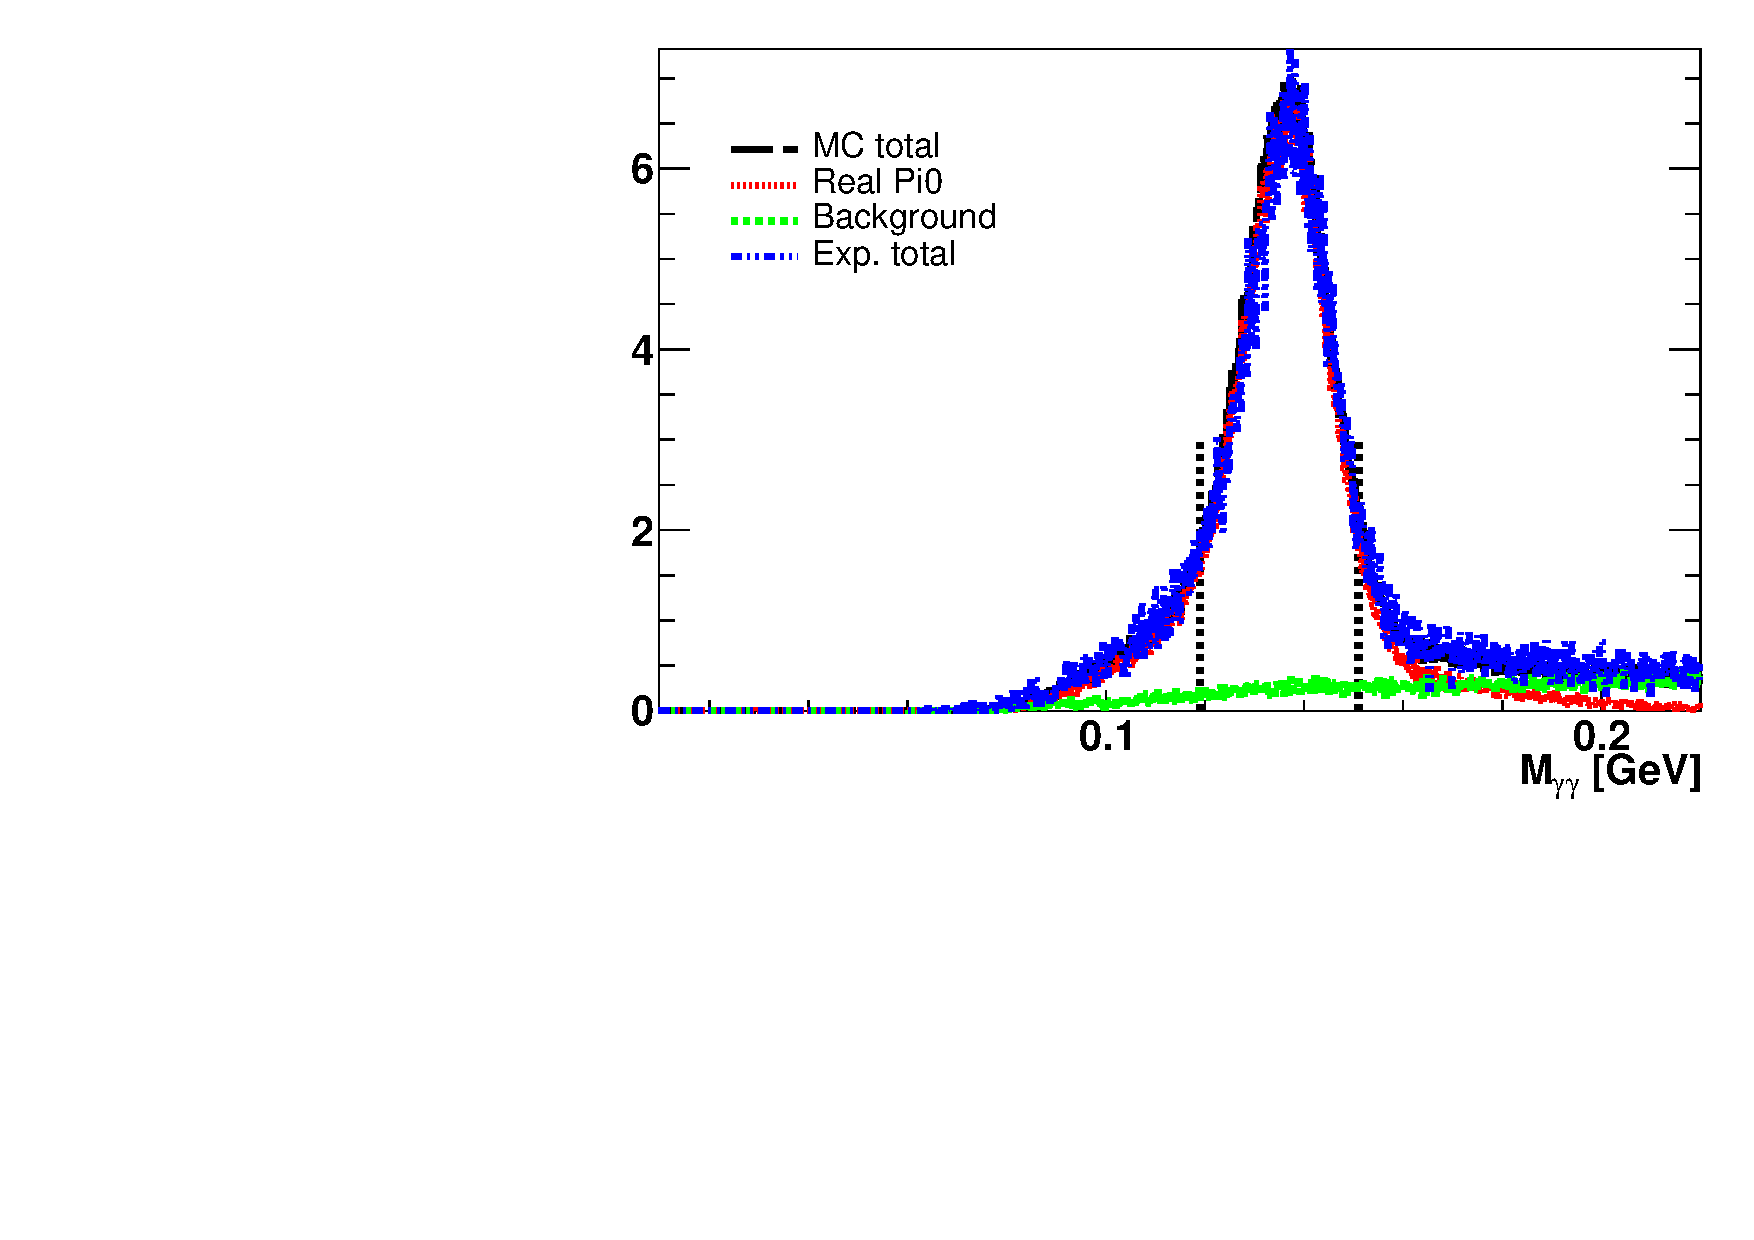
\includegraphics[width=.48\textwidth,natwidth=250,natheight=100]{figure_dataselection/pi0_Z_5.pdf}}
      \caption[Invariant mass of Monte Carlo vs.~experimental data for some exemplary bins]{Invariant mass of Monte Carlo vs.~experimental data for some exemplary bins after applying all fiducial and energy constraints. The black line is the total Monte Carlo invariant mass. The blue line is the experimental invariant mass. The red line is the real $\pi^0$ signal identified by particle ID from Monte Carlo and the green line represents background in Monte Carlo. We define an identified photon pair as a ``real'' $\pi^0$ if both corresponding true particles have a common $\pi^0$ as a parent. The vertical dash lines are the boundaries of the signal invariant mass window.}
  \label{fig:pi0MC_Exp}
\end{figure}


To address this problem of the overestimation of the signal region yield in the simulation, we divide the invariant mass range into upper and lower sidebands as well as a signal region. Our approach will be to fix the signal/bg ratio in the sideband regions, where the agreement is quite good and extrapolate the background under the signal peak.
The range of the lower sideband is $0.014$~GeV$\textup{--}0.112$~GeV. In this region, shapes of both simulation and data agree. Hence, for this region, experimental background is estimated using Eq.~\eqref{eqn:pi0fitfunction1}, in which $N_i^{bg}$ is the experimental background of invariant mass bin $i$ and $N_i^{tot}$ is the experimental total yield of bin $i$. $N_i^{MCtot}$ and $N_i^{MCbg}$ represent the MC and MC background content of bin $i$, respectively:
\begin{equation}
N_i^{bg}=\frac{N_i^{tot}}{N_i^{MCtot}}*N_i^{MCbg}.
\label{eqn:pi0fitfunction1}
\end{equation}
In other words, we assume the same background fraction in the MC simulation and the experimental data and thus apply the one obtained from the MC simulation to the experimental-data yields in order to obtain the experimental BG yield, and do that for each invariant-mass bin separately.


As shown in Fig.~\ref{fig:pi0MC_Exp} experimental data and MC have the similar shape in the upper sideband region from $0.146$~GeV to $0.22$~GeV and we therefore also use Eq.~\eqref{eqn:pi0fitfunction1} to fit this region. The idea of background fitting is a simple conversion between MC to experimental data.

The signal region is $0.112$~GeV$\textup{--}0.146$~GeV. As the shapes of MC and experimental data are quite different, especially the peak position changes slightly, a simple conversion doesn't work here. Fortunately the background in this section is smooth in MC and a polynomial function of order 2 connecting upper and lower sidebands can be used to estimate background.
The fit connecting the upper and lower sidebands uses 20 points on each side covering $\pm 0.02$ on each side.

Finally, the signal is obtained by subtracting the background shape from the experimental data. Fig.~\ref{fig:pi0_fit} shows the fit result of $\pi^0$.  

\begin{figure}
  \centering     
  \subfigure[$\pi^0$ invariant mass fit, $P_t<0.15$~GeV]{\label{fig:pi0fit_1}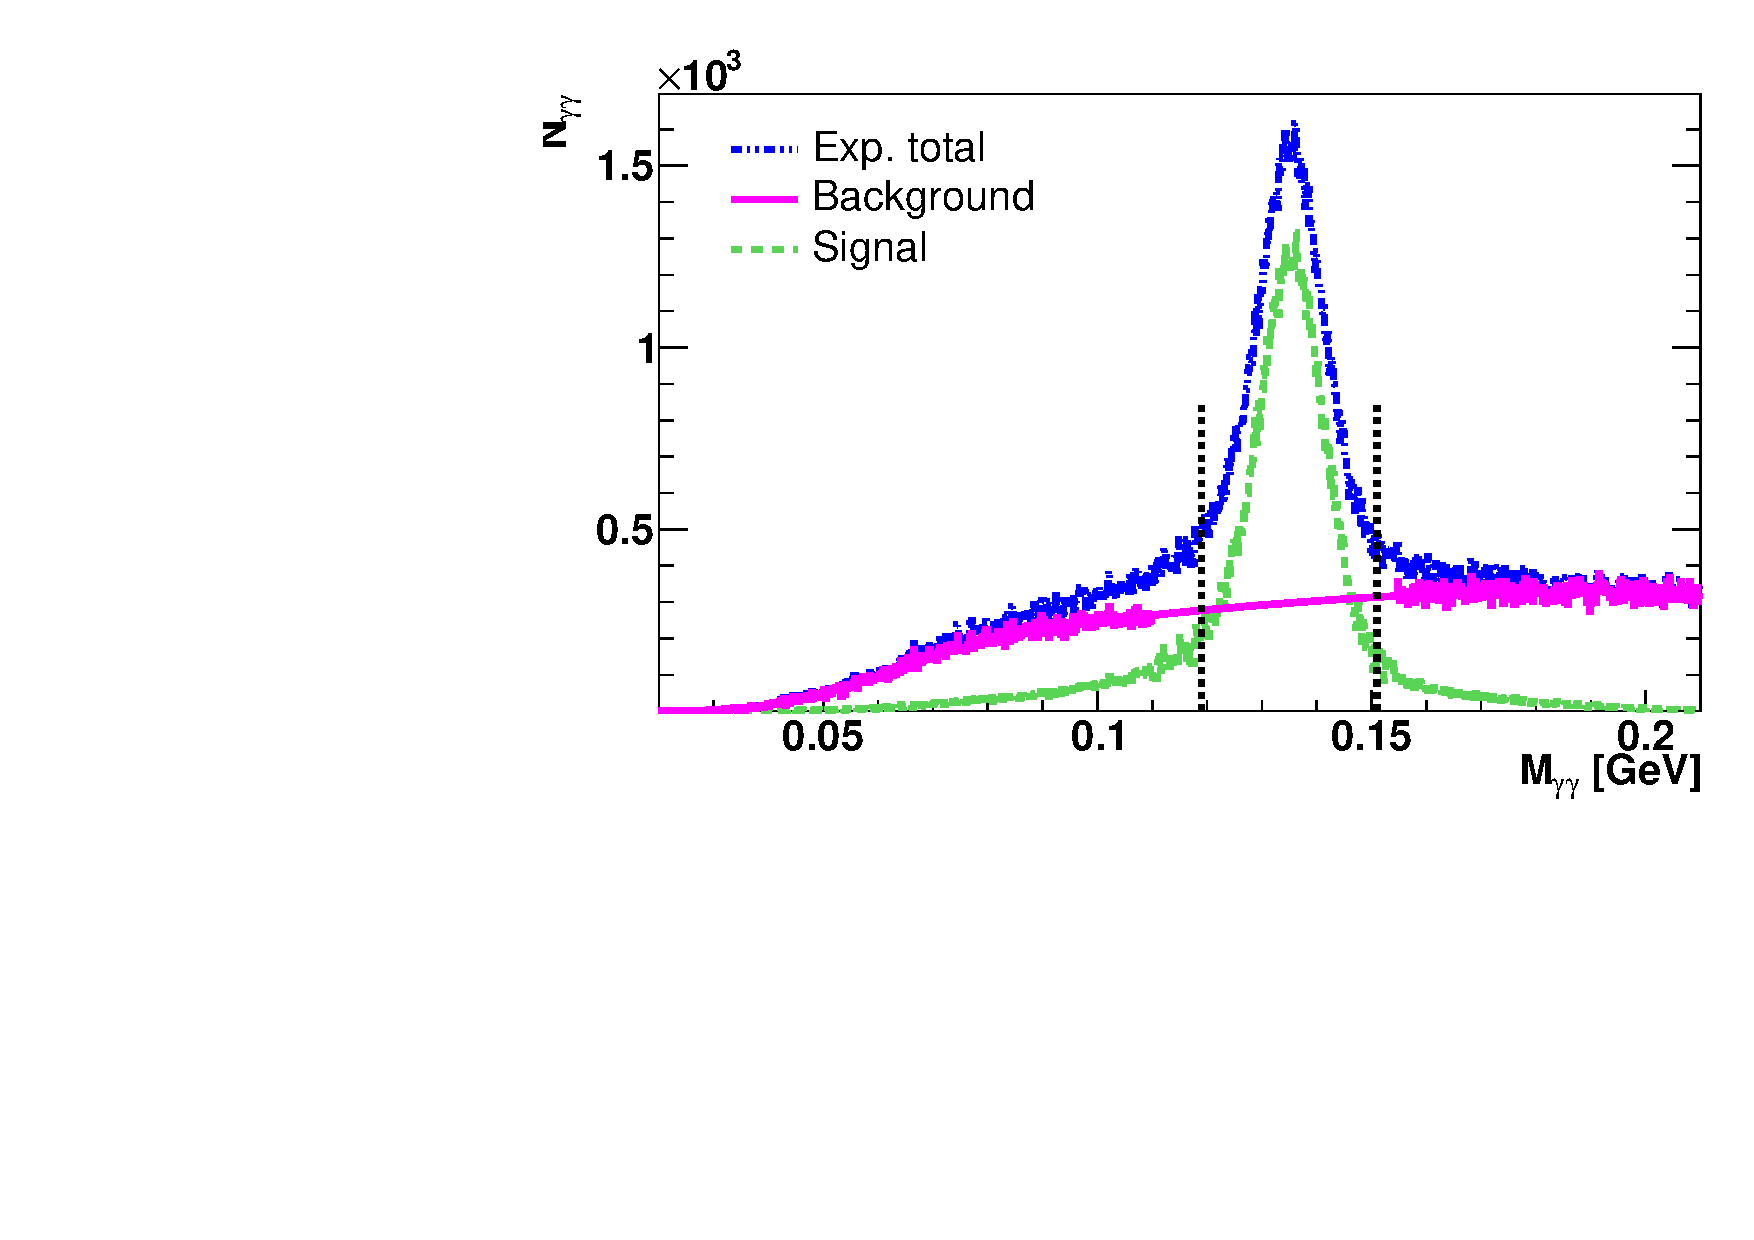
\includegraphics[width=.48\textwidth,natwidth=600,natheight=400]{figure_dataselection/pi0_fit_Pt_0.pdf}}
  \subfigure[$\pi^0$ invariant mass fit, 0.3~GeV $<P_t<0.5$~GeV]{\label{fig:pi0fit_2}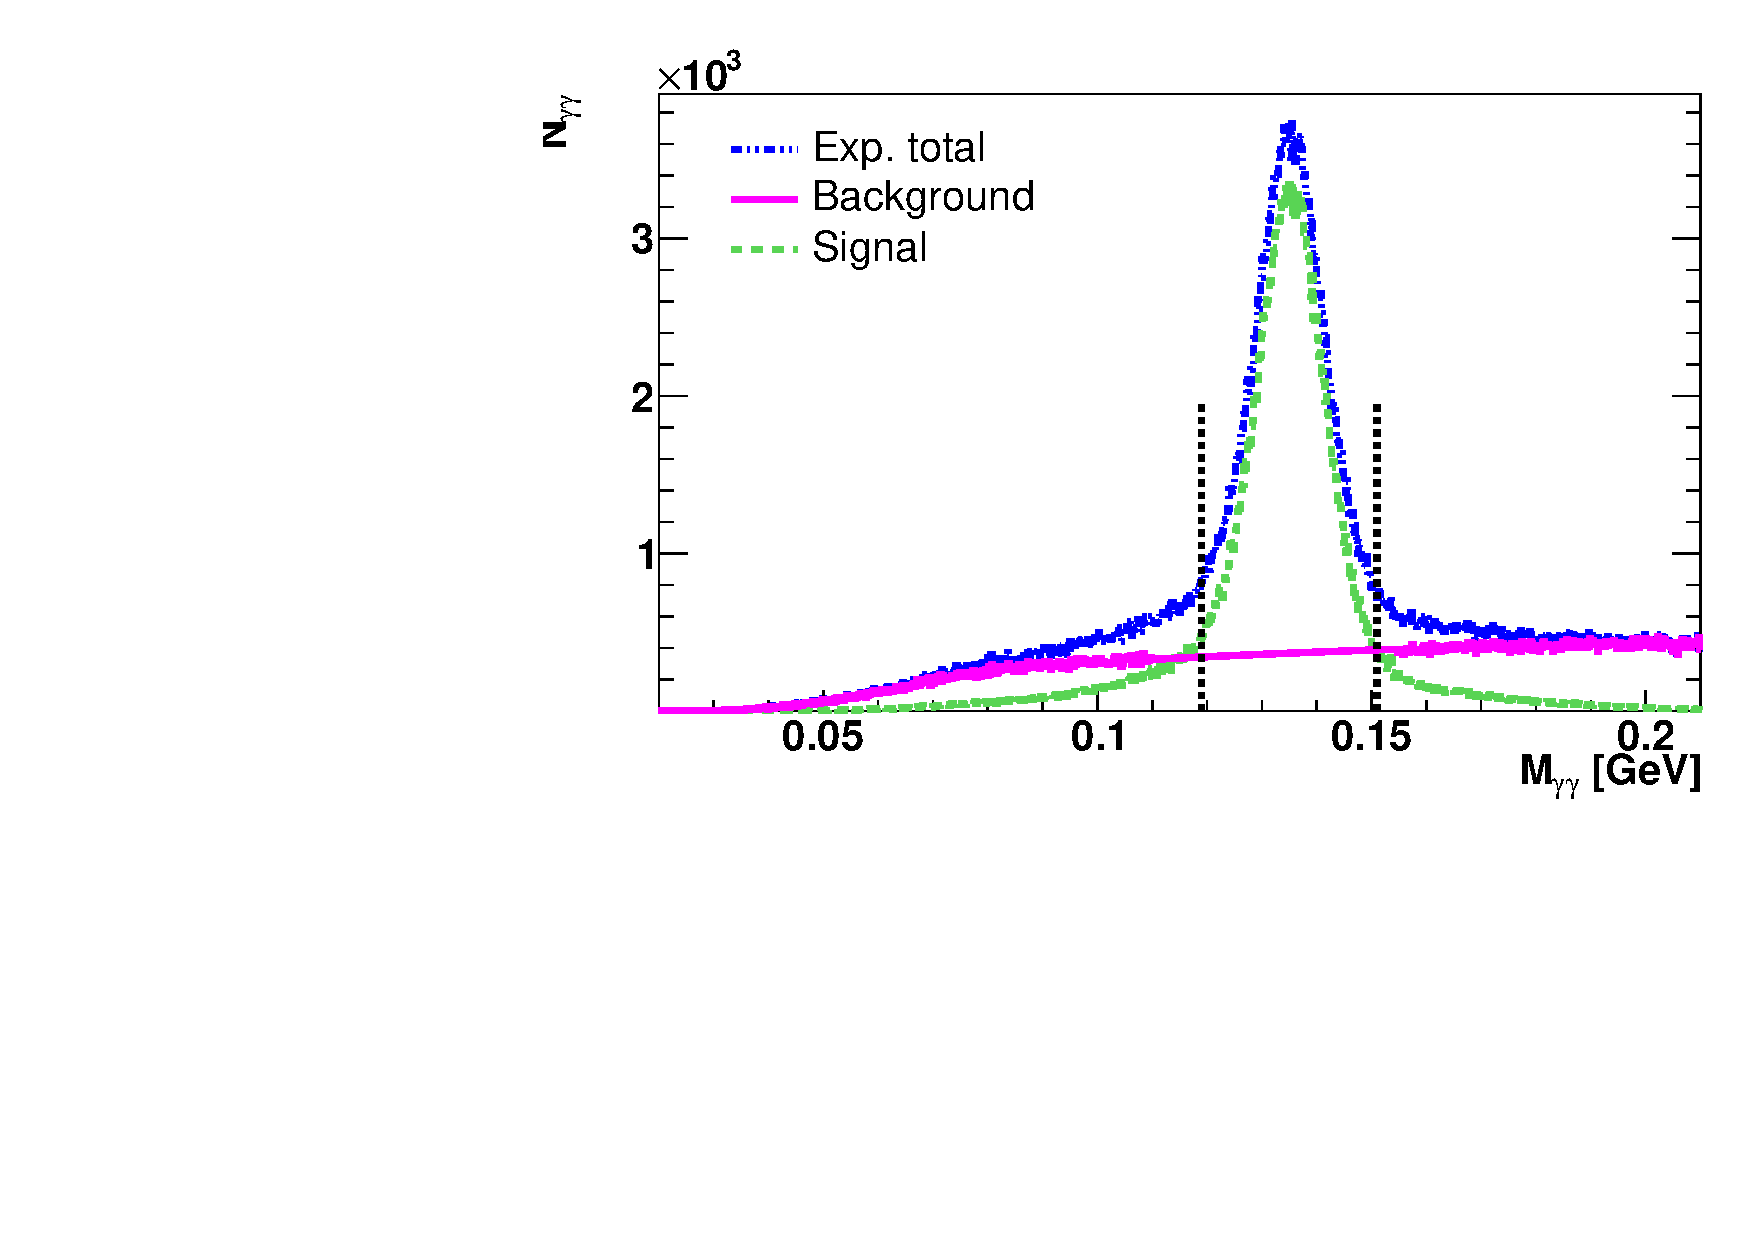
\includegraphics[width=.48\textwidth,natwidth=600,natheight=400]{figure_dataselection/pi0_fit_Pt_2.pdf}}
  \subfigure[$\pi^0$ invariant mass fit, $0.2<z<0.3$]{\label{fig:pi0fit_3}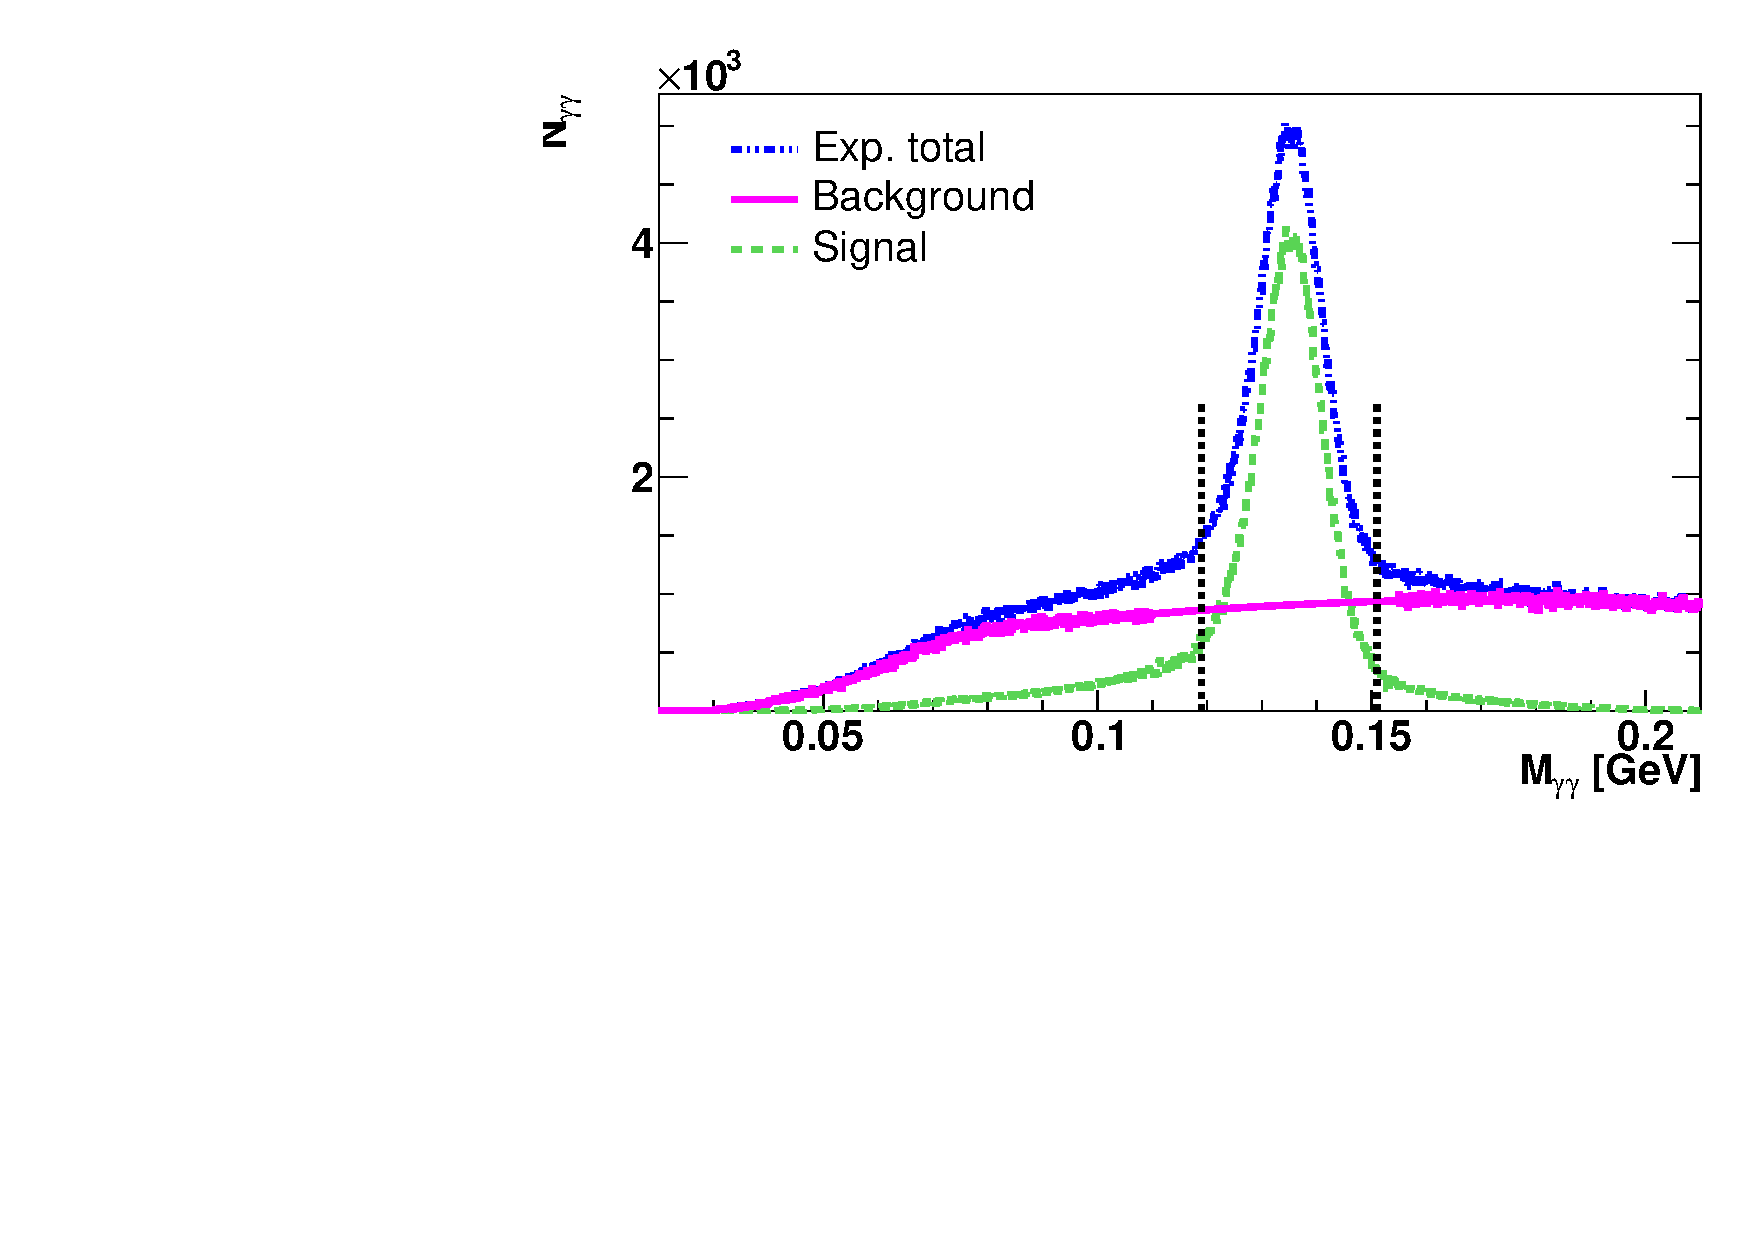
\includegraphics[width=.48\textwidth,natwidth=600,natheight=400]{figure_dataselection/pi0_fit_Z_1.pdf}}
  \subfigure[$\pi^0$ invariant mass fit, $0.6<z<0.7$ ]{\label{fig:pi0fit_4}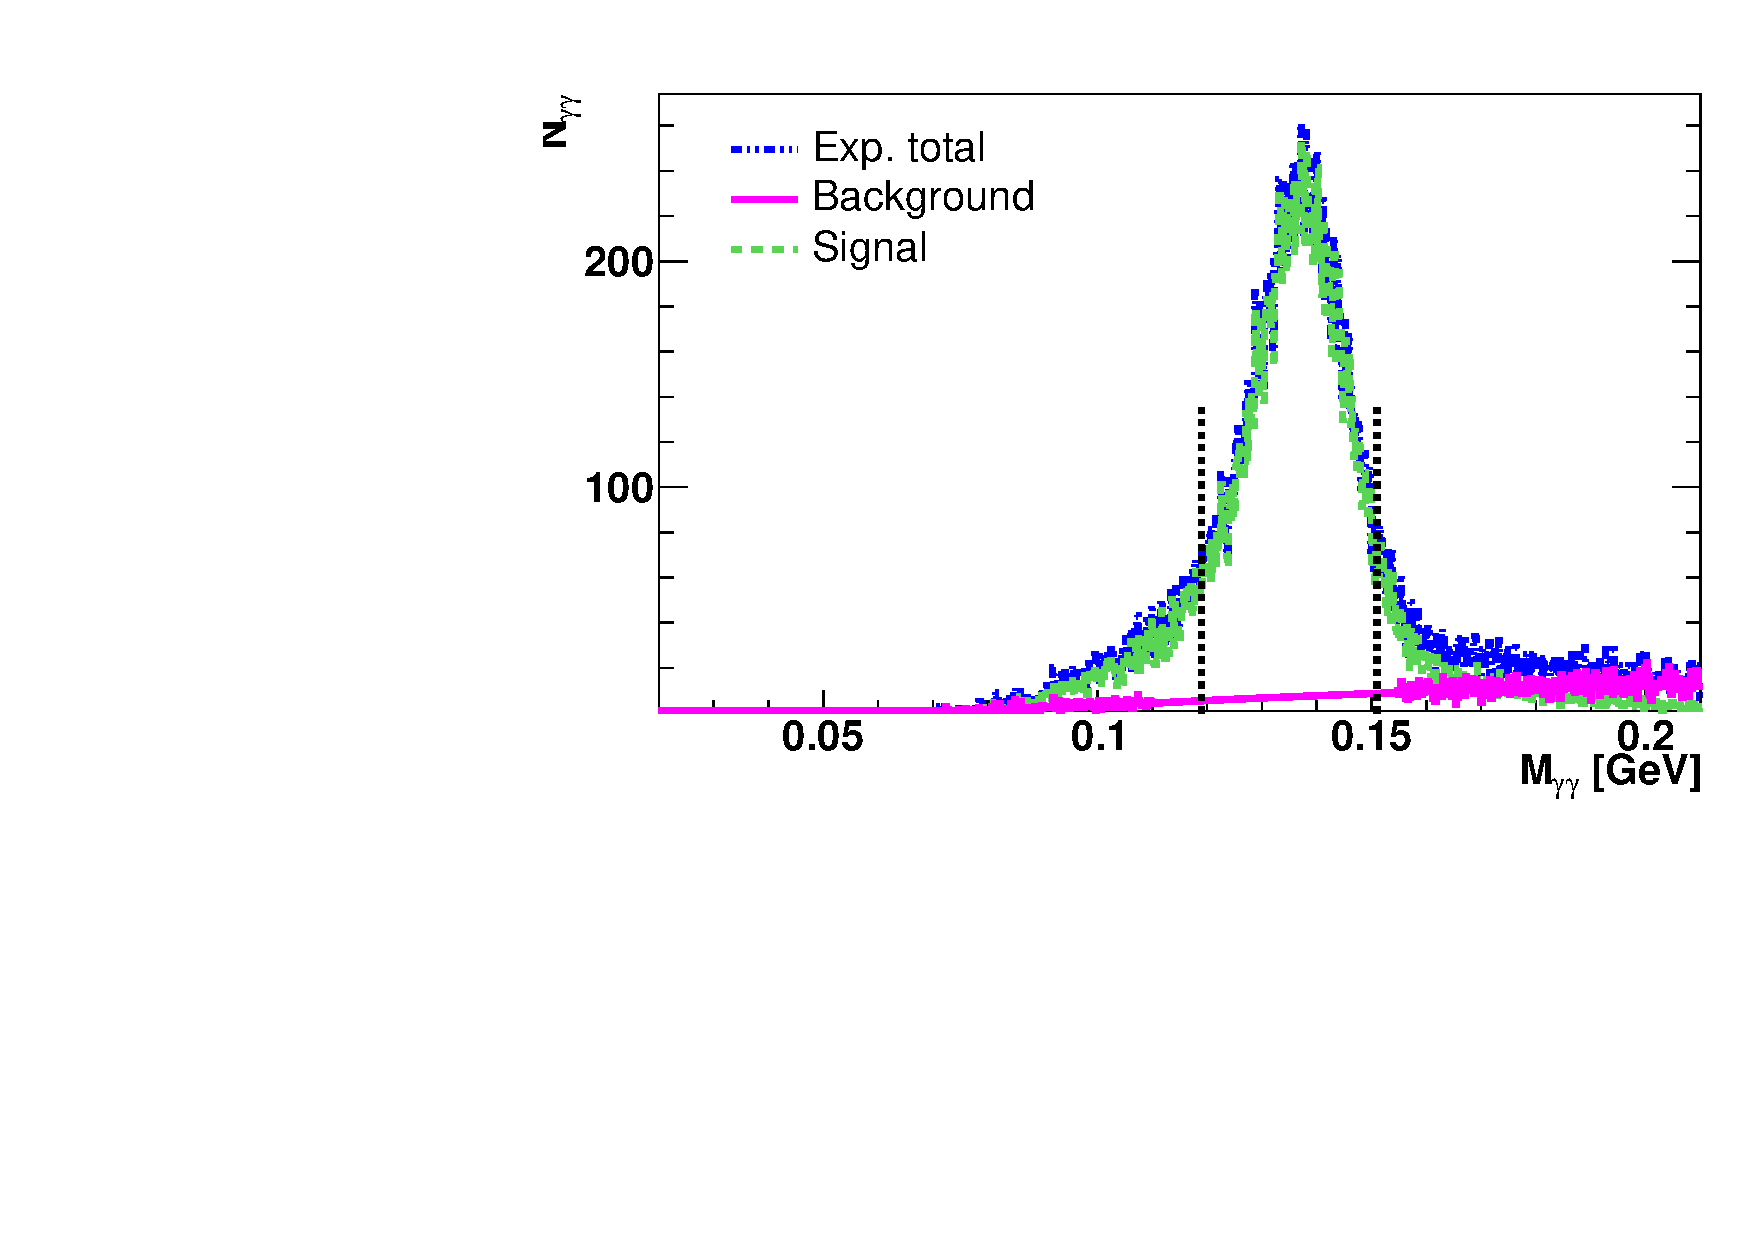
\includegraphics[width=.48\textwidth,natwidth=600,natheight=400]{figure_dataselection/pi0_fit_Z_5.pdf}}
  \caption[Nonparametric fit of the experimental data using the Monte Carlo background shape]{Nonparametric fit of the experimental data using the MC background shape. The blue line is the total experimental data. The purple line is the background which has the same shape with background in MC. The green dash line is the signal obtained by subtracting the background from the total yield in the signal region. The vertical dash line is again the signal window. }
  \label{fig:pi0_fit}
\end{figure}

In order to evaluate the parametric Crystal-Ball and the non-parametric methods for the $\pi^0$ extraction presented in this section, we compare the obtained signals in Fig.~\ref{fig:pi0mcexpsig} with the signal from the simulation. 
Note that here the signal in Monte Carlo also comes from the direct reconstruction of the $\gamma$'s instead of using the $\pi^0$ particle table provided by the Belle MC. Section~\ref{sec:sysStudies} discusses the signal and background identification in some more detail. In short, we define all reconstructed $\gamma$ pairs as background, where the corresponding true particles cannot be traced back to a common $\pi^0$ parent (or $\eta$ when we want to reconstruct those, but in this channel the backgrounds are small). 

The results in Fig.~\ref{fig:pi0mcexpsig} show a discrepancy in the extracted signals between the methods in the lower $z$ and $P_t$ bins. In particular, the MC signal shape has longer tails towards lower invariant masses. This leads to a lower estimation of the background in the signal region, which in turn leads to a larger extracted signal compared to the Crystal-Ball method. The MC signal is larger than both methods, reflecting the data-simulation difference. The data/MC difference only impacts the non-parametric method. We think that assigning the difference between the two methods as a systematic effect captures a signal shape that is different from the Crystal-Ball method (assumed for the parametric method) and potential effects from the data/mc disagreement on the non-parametric method. It should be noted that we show later in Section~\ref{sec:backgroundcorrection} that the sidebands also carry an asymmetry that is close to the signal region. This helps suppress any systematic effect on the estimation of the signal fraction.
%Given that the sidebands also carry a sizeable asymmetry that is actually of similar magnitude than the signal region (see sec.~\ref{sec:backgroundcorrection} ), we think that the any effect of the data/mc difference 

%In Fig.~\ref{fig:pi0mcexpsig}, the signal region in the experimental data exceeds the signal distribution in the MC simulation for the lower $z$ bins. This can already be seen in the total invariant-mass distributions.
% In addition, the two extraction methods give different signals.The high-z bin presented shows better agreement of the $\pi^0$ peaks. 
%Section~\ref{sec:backgroundcorrection} shows that because the background has asymmetries at the same level as signal the uncertainty of purity, defined as signal over total data, does not contribute much to the systematic uncertainty. 

%For the final results we use the Crystal Ball fit 

%Since there is evidence that the simulated background shape agrees with experiment, e.g. from the sidebands in fig.~\ref{fig:pi0_fit} and our studies presented in sec.~\ref{sec:backgroundcorrection} show that the sidebands have in fact a similar 
%Since the background shapes on the other hand show good agreement between data and MC and we know from Section~ that uncertainties in the purity in the signal region can be neglegted due to the similar size of the background and signal asymmetries, we do not consider data-MC difference in the MC region for small $z$ in our systematic uncertainties. We think that any differences between data and simulation are mainly important for the background estimation and are captured in assigning the difference between the two fit methods as a systematic uncertainty.

 The Crystal Ball method leads to a proper fitting result of $\eta$, see section~\ref{sec:etafitsection}, so in order to make the analysis consistent we adopt the Crystal Ball method for $\pi^0$ as well. The difference between the two signal extraction methods will be included as part of systematic uncertainties.
\begin{figure}
  \centering     
  \subfigure[ $0$~GeV$<P_t<0.15$~GeV]{\label{fig:pi0mcexpsig_1}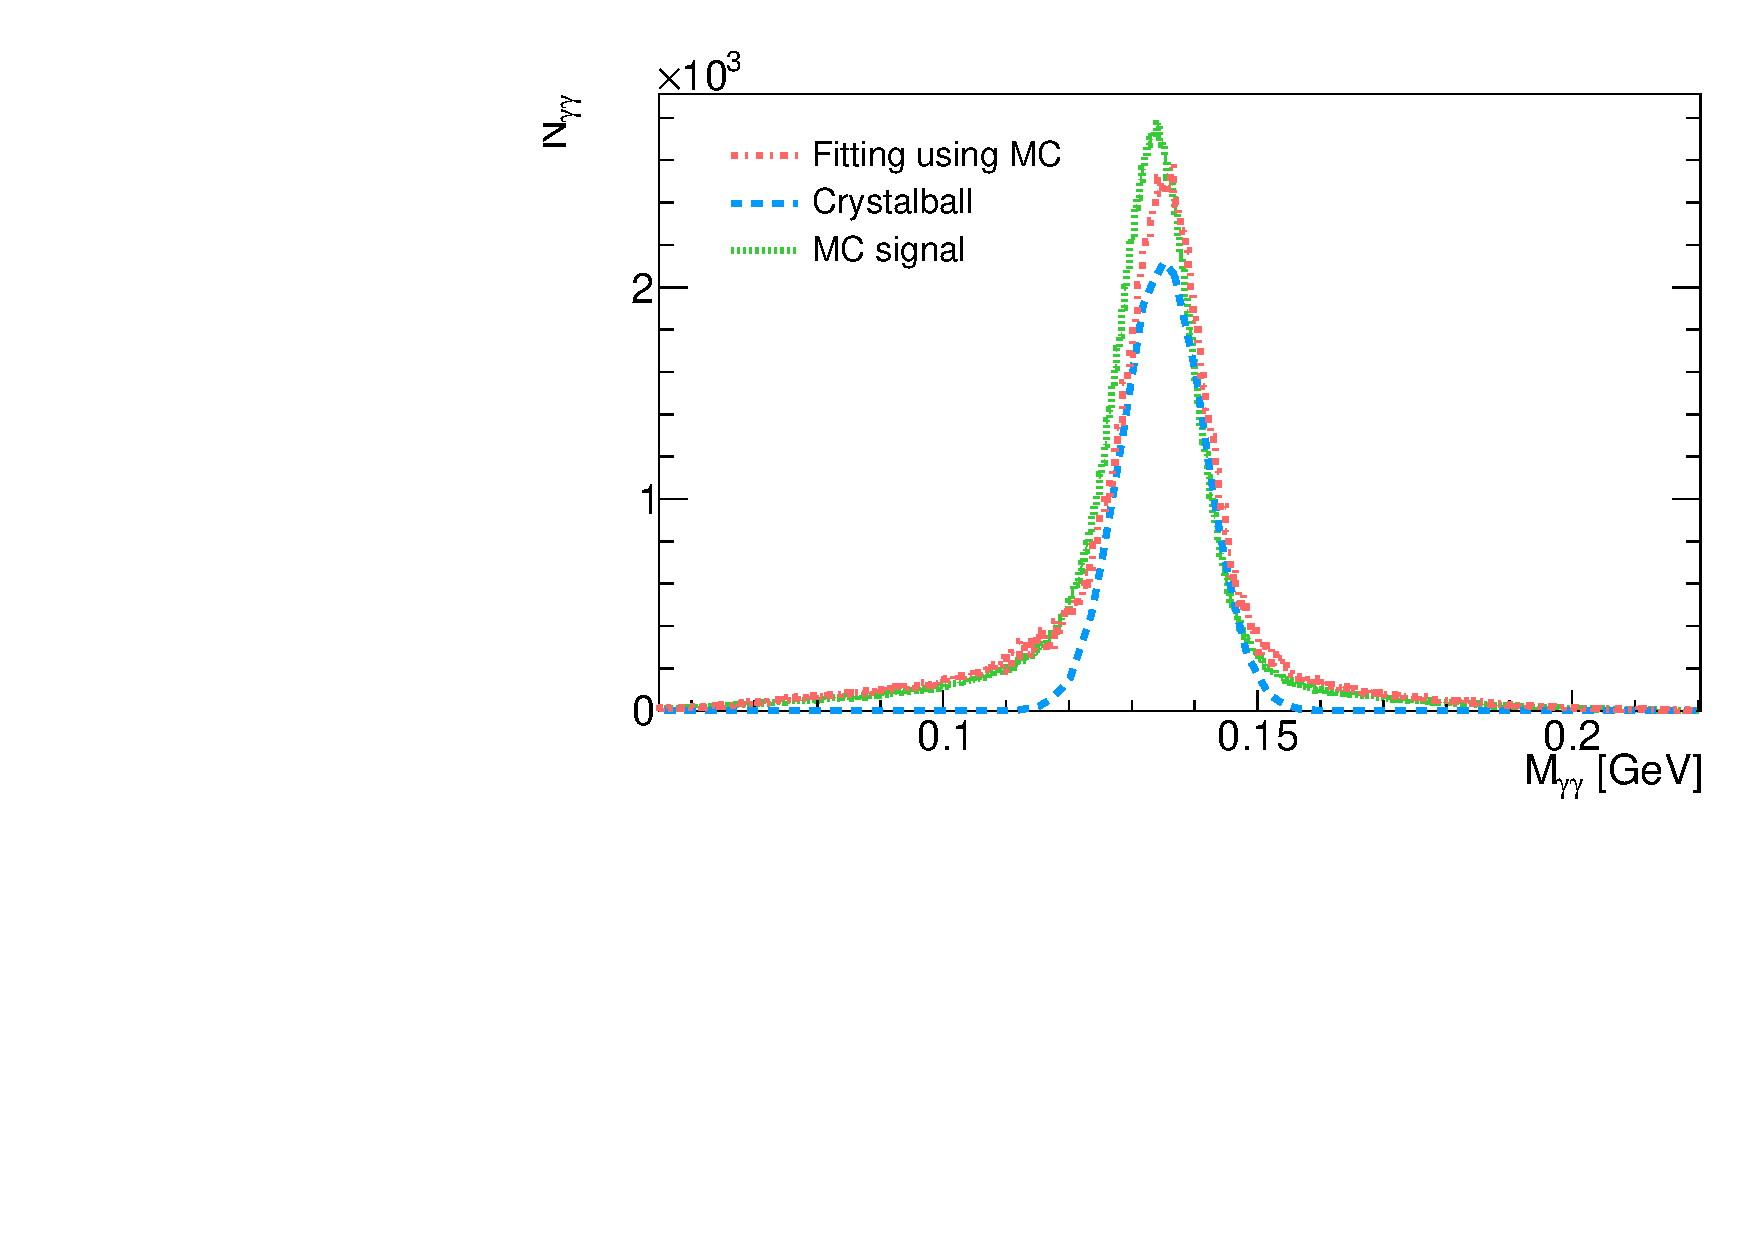
\includegraphics[width=.48\textwidth,natwidth=600,natheight=400]{figure_dataselection/fitting_signal_compare_Pt0.pdf}}
  \subfigure[$0.3$~GeV$<P_t<0.5$~GeV]{\label{fig:pi0mcexpsig_2}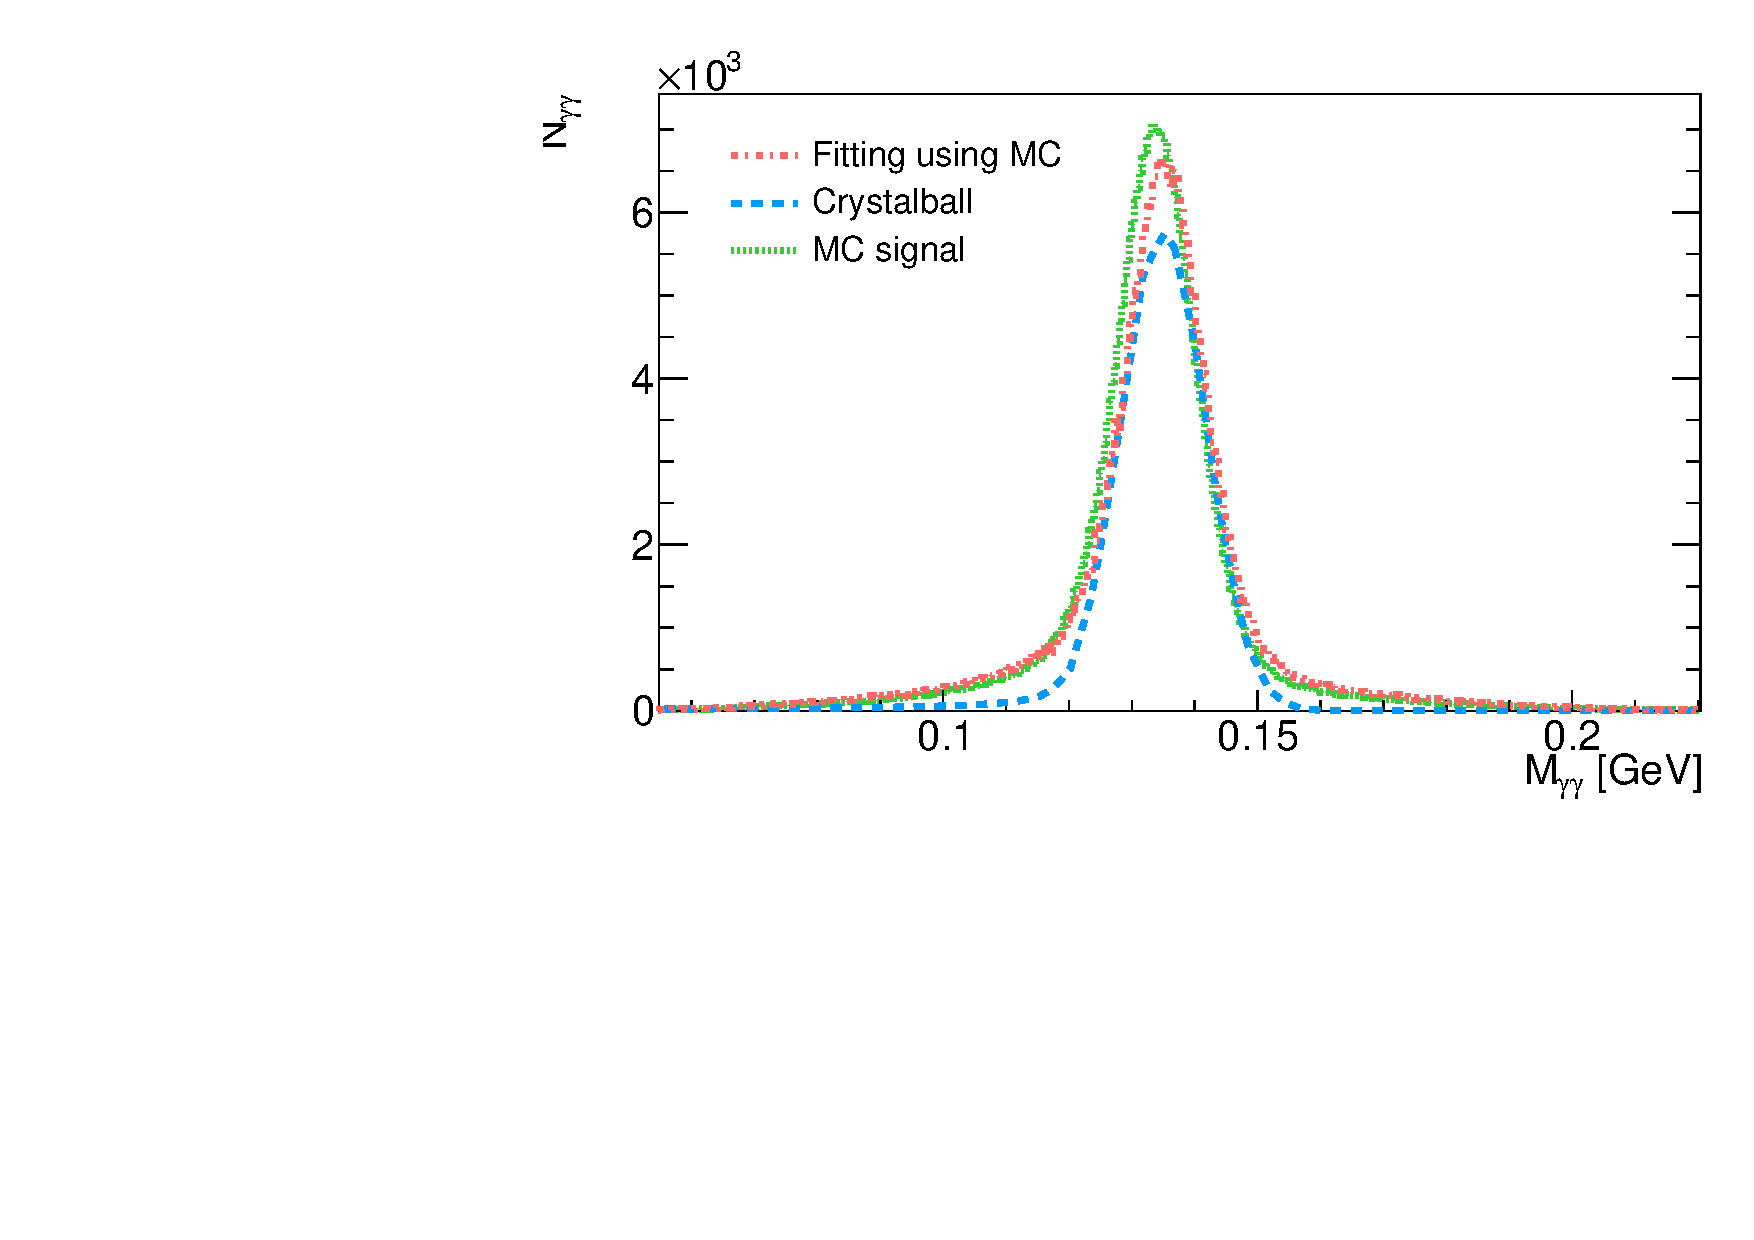
\includegraphics[width=.48\textwidth,natwidth=600,natheight=400]{figure_dataselection/fitting_signal_compare_Pt2.pdf}}
  \subfigure[$0.2<z<0.3$]{\label{fig:pi0mcexpsig_3}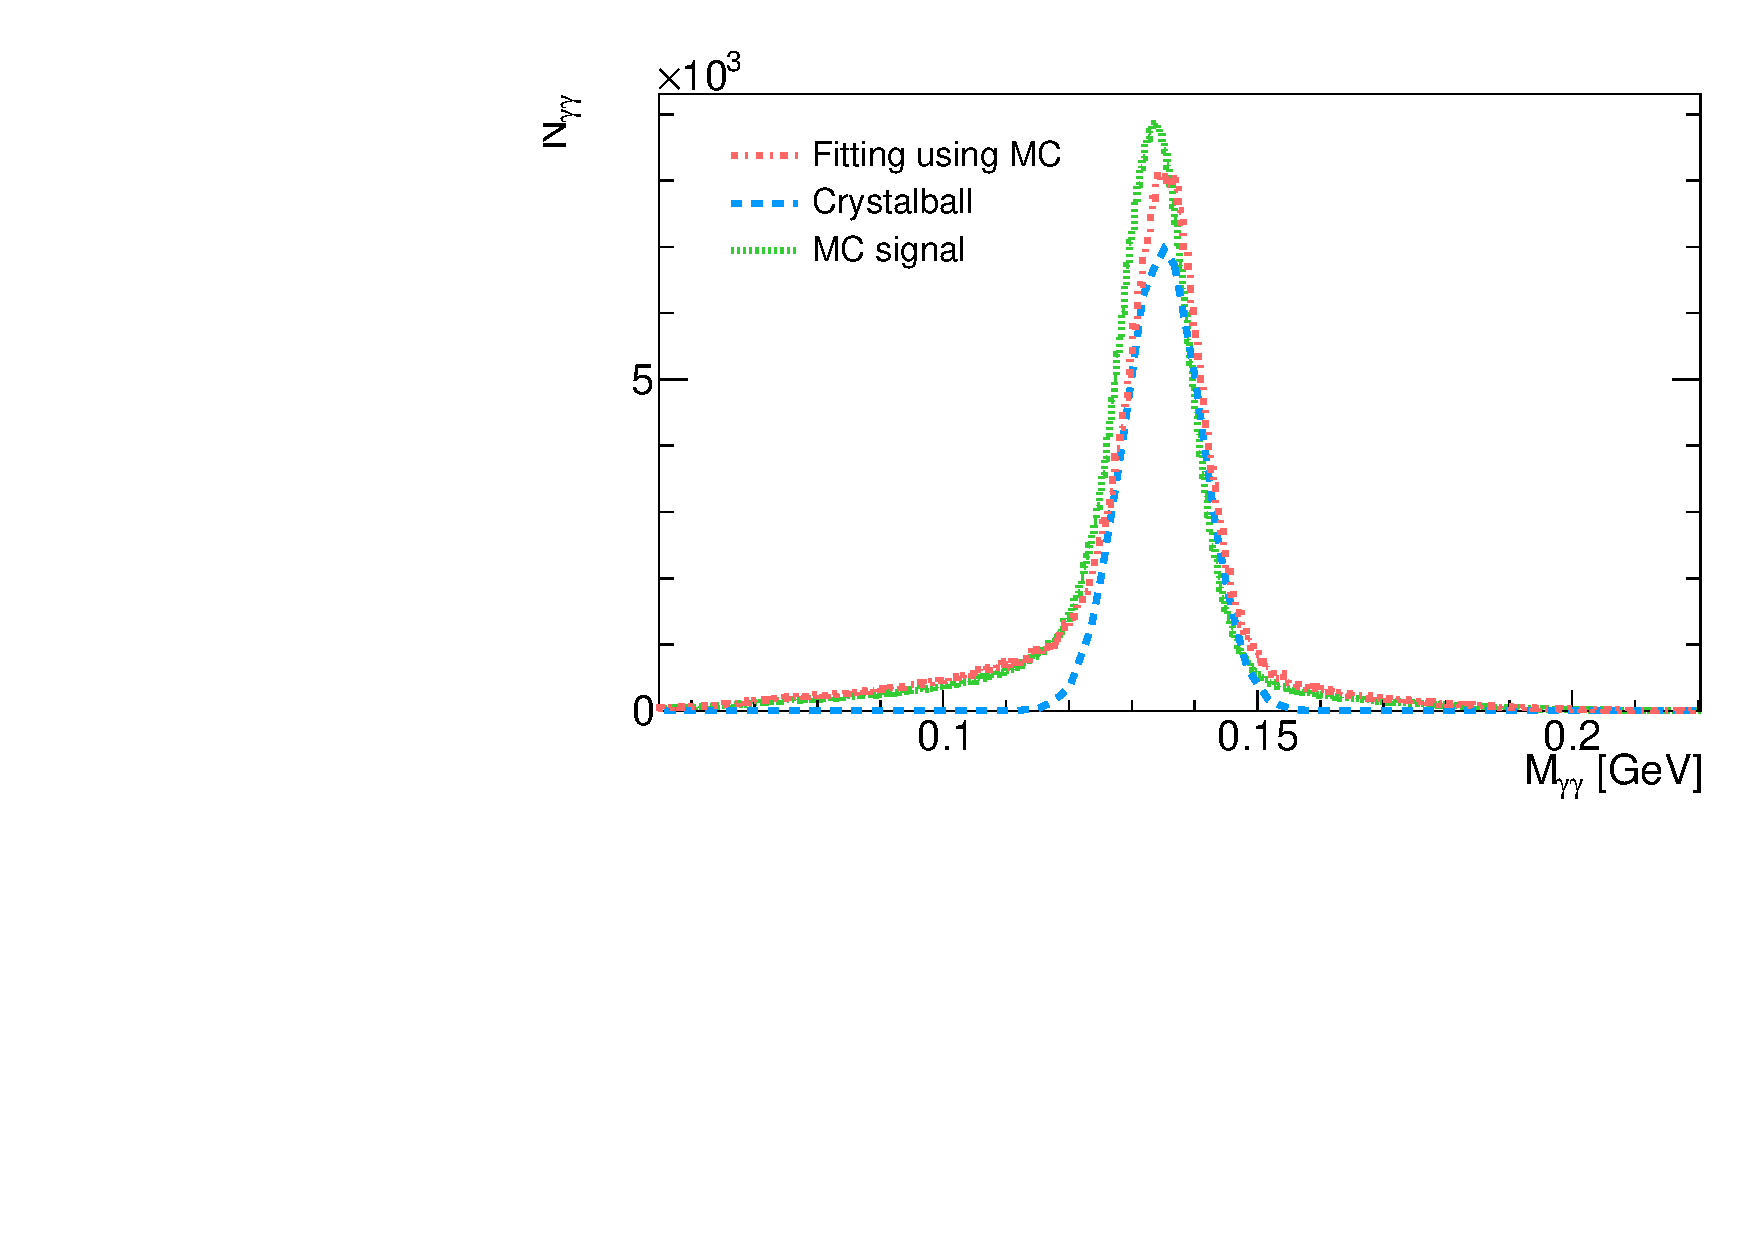
\includegraphics[width=.48\textwidth,natwidth=600,natheight=400]{figure_dataselection/fitting_signal_compare_Z1.pdf}}
  \subfigure[$0.6<z<0.7$]{\label{fig:pi0mcexpsig_4}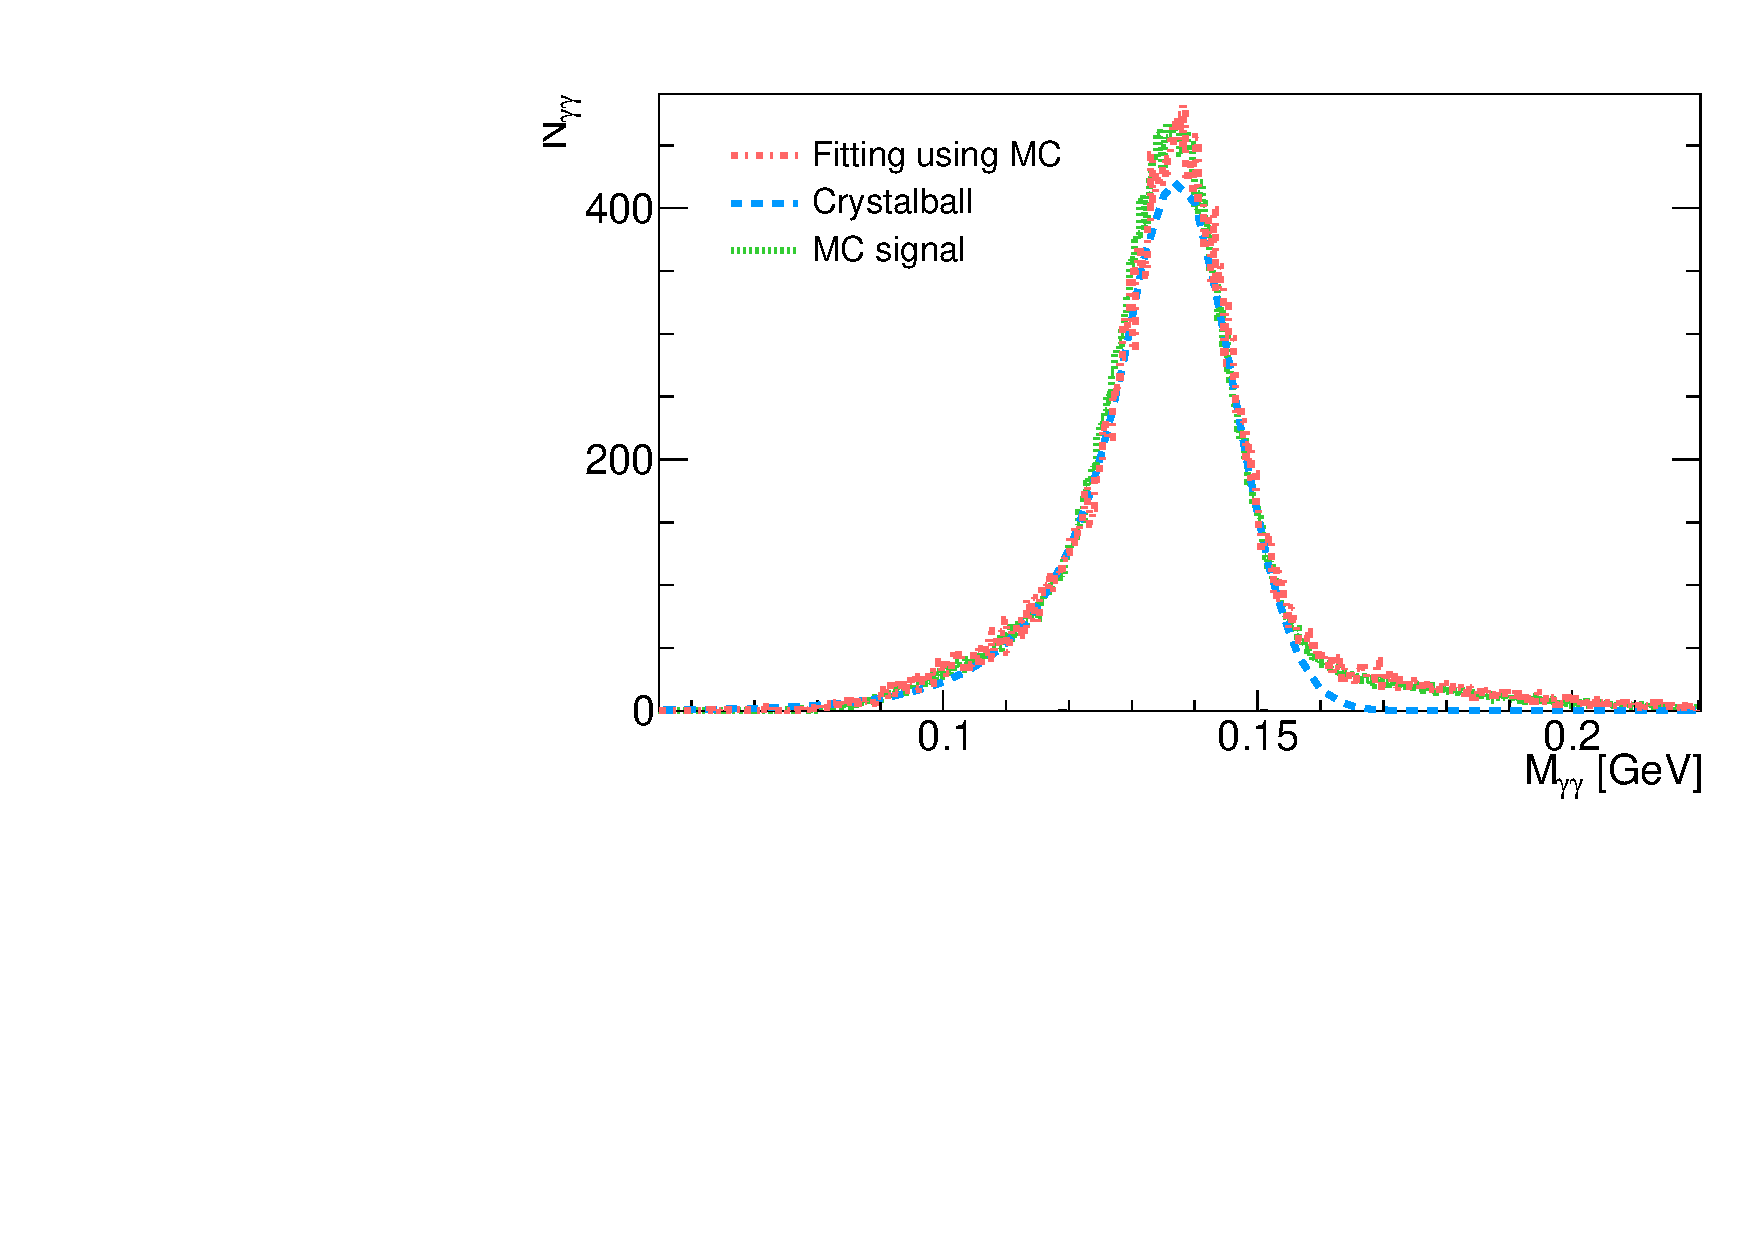
\includegraphics[width=.48\textwidth,natwidth=600,natheight=400]{figure_dataselection/fitting_signal_compare_Z5.pdf}}
  \caption[Signals from Monte Carlo and experiment]{Signals from Monte Carlo and experiment. The green line is the Monte Carlo $\pi^0$ signal and the  red/blue line are the experimental signal.}
  \label{fig:pi0mcexpsig}
\end{figure}

\subsubsection{\texorpdfstring{Invariant-Mass Fit of $\eta$}{eta fit} }
\label{sec:etafitsection}
The background shape under the $\eta$ peak is consistent between the upper and lower sidebands, in fact it can almost be described as a linear function. In the spirit of the previous section, we tried two different approaches. 
In the first, we fit the background separately in the upper and lower sidebands, 
%(046.~GeV-0.45~GeV and 0.6~GeV-0.69~GeV), 
extrapolated through the signal region, and obtained the signal by subtracting the background from the total data. 
The second method is the same as the one used for the $\pi^0$ case and described above: 
We use a fifth-order polynomial together with a Crystal-Ball function (see Eqn.~\eqref{eqn:crystalball} and Ref.~\cite{CrystalBallFunc}) to fit background and signal simultaneously. 


\begin{figure}
\centering     %%% not \center
\subfigure{\label{fig:etaz4fitbkg}\includegraphics[width=.48\textwidth,natwidth=600,natheight=400]{figure_dataselection/eta_fitbkg_Z_4.pdf}}
\subfigure{\label{fig:etaz4fitall}\includegraphics[width=.48\textwidth,natwidth=600,natheight=400]{figure_dataselection/eta_fitall_Z_4.pdf}}
\caption[Fits of $\eta$ invariant mass for $z$ bin 4 in experimental data]{Fits of $\eta$ invariant mass for $z$ bin 4 ($0.5<z<0.6$) in experimental data. Left: the black line is the total experimental data, the green dotted line is a fourth-order polynomial and the blue line is the signal obtained by subtracting the red line from all data. Right: the black line is the total data, the red line is the Crystal Ball fit, the green line is a fifth-order polynomial, and the turquoise line is the sum of signal and BG fit.}
\label{fig:eta_fit}
\end{figure}

Figure~\ref{fig:eta_fit} shows the fit results and Fig.~\ref{fig:etasignal} displays the signals arising from those two methods for the specific bin $0.5 < z < 0.6$. It can be seen that these methods give similar fitting results. However, for consistency reasons we use the Crystal Ball function plus the 5th order polynomial, since the same function can also be used to fit the $\pi^0$.

\begin{figure}
\centering
\includegraphics[width=0.5\textwidth,natwidth=610,natheight=642]{figure_dataselection/eta_Signal_Z_4.pdf}
\caption[Comparison of $\eta$ signal extractions]{Comparison of $\eta$ signal extractions for $0.5<z<0.6$: Red line is the result of the Crystal-Ball fit. Blue line is the signal from subtracting the background fit from the total distribution.}
\label{fig:etasignal}
\end{figure}

%%%%%%%%%%%%%%%
\subsubsection{\texorpdfstring{Mass Window to Select $\pi^0$ and $\eta$}{Mass Window to Select pi0 and eta}}
\label{sec:masswindow}

In this section we describe how we choose the optimal mass window in the two-photon invariant-mass spectrum 
to select $\pi^0$ and $\eta$. The obvious issue is that a smaller mass window will lead to a higher signal-to-background ratio but also to a reduction in signal yield. Figure~\ref{fig:pi0ST} shows the relative signal contribution for various mass ranges. Figure~\ref{fig:pi0SST} shows the $S/\sqrt{N}$ ratio, which is the figure of merit (FOM) we use, of different mass-window widths for $\pi^0$, where $N$ is the total  and $S$ the signal yield. The mass window is centered around 0.135~GeV, which is the world average mass for the  $\pi^0$. We define the mass window width to be half  the mass range. For example with width 0.005, the mass window is 0.130~GeV -- 0.140~GeV. Both purity and yield factors are taken into account when selecting the mass window. Figure~\ref{fig:etaS} shows the FOM of $\eta$.
\begin{figure}
\centering     %%% not \center
\subfigure[$S/N$ ratio of $\pi^0$]{\label{fig:pi0ST}\includegraphics[width=60mm]{figure_dataselection/pi0_signal_ratio_crystalballfit.eps}}
\subfigure[$S/\sqrt{N}$ ratio of $\pi^0$]{\label{fig:pi0SST}\includegraphics[width=60mm]{figure_dataselection/pi0_STT_ratio_crystalballfit.eps}}
\caption[Two ratios of signal and background yields related to the $\pi^0$ mass window selection]{Two ratios related to the $\pi^0$ mass window selection. Different colors/line styles are ratios for different $z$ and $P_t$ bins. The horizontal axis is mass-window width~(see text for details).}
\label{fig:pi0S}
\end{figure}

\begin{figure}
\centering     %%% not \center
\subfigure[$S/N$ ratio of $\eta$]{\label{fig:etaST}\includegraphics[width=.45\textwidth,natwidth=250,natheight=100]{figure_dataselection/eta_signal_ratio.pdf}}
\subfigure[$S/\sqrt{N}$ ratio of $\eta$. Note that the {\bf $y$ axis is mislabeled} and should read $S/\sqrt{N}$]{\label{fig:etaSST}\includegraphics[width=.45\textwidth,natwidth=250,natheight=100]{figure_dataselection/eta_STT_ratio.pdf}}
\caption[Two ratios of signal and background yields related to the $\eta$ mass window selection]{Two ratios related to  the $\eta$ mass window selection. Different colors/line styles are ratios for different $z$ and $P_t$ bins. The horizontal axis is mass-window width~(see text for details).}
\label{fig:etaS}
\end{figure}
The final mass windows were chosen as
\begin{itemize}
\item $\pi^0$ mass range: 0.119~GeV -- 0.151~GeV,
\item $\eta$ mass range: 0.5238~GeV -- 0.5718~GeV.
\end{itemize}
